\chapter{Displaced Jet Analysis \label{ch:analysis}}

\section{Introduction}

The study of physics beyond the standard model (BSM) is one of the main
objectives of the ATLAS and CMS experiments at the CERN LHC. With no
signal observed so far, the ATLAS and CMS results put severe bounds on
BSM theories.

The majority of these searches focus on prompt particles with
lifetimes $c\tau_0<1$mm and contain requirements on the
physics objects that reject longer lived particle
decays. This leaves open the possibility that light long-lived particles
could exist and still remain undetected.  In this paper, we present an
inclusive search for long-lived particles decaying to various
combinations of jets and leptons. The analysis exploits the
information originating from the CMS calorimeters to reconstruct jets
and measure their energies. The information from reconstructed tracks,
in particular the transverse impact parameters, is used to
discriminate the displaced-jets signal from the background of ordinary
multijet events.  The analysis is performed on data collected with the
CMS detector at a center-of-mass energy $\sqrt{s}=13$~TeV in 2015. The
data set corresponds to an integrated luminosity of
2.7fb$^{-1}$. Results for similar signatures have been reported by
ATLAS~\cite{PhysRevD.92.012010,Aad:2015rba} and
CMS~\cite{CMS:2014wda}, using data collected at $\sqrt{s}=8$~TeV.

\section{Datasets} 

\section{Coordinate Conventions}

\framebox{Pseudorapidity $\eta$} As the detector has cylindrical symmetry, the coordinate system used most commonly is two dimensional $(\eta, \phi)$. The pseudo-rapidity, $\eta$ is an approximation to rapidity, $y$, that is exact in the $\beta = 1$ limit:
\begin{align*}
y = \frac{1}{2}\log \frac{E - p_z}{E+p_z}\hspace{.75in} \eta = - \log \left( \tan\left (\frac{\theta}{2} \right ) \right)  
\end{align*}
where $\theta$ is the angle from the positive beam axis. This variable is useful for a number of reasons. Firstly, differences in rapidity are invariant under longitudinal lorrentz boosts along the beam axis. Also, for the energies being probed the particles in the decay products are of negligible mass and the approximation $\eta \approx y$ is nearly exact. Given this relation, pseudorapidity provides an intuitive geometric interpretation. Near full solid angle coverage is provided within $|\eta| < 5$

\begin{figure}
\begin{center}
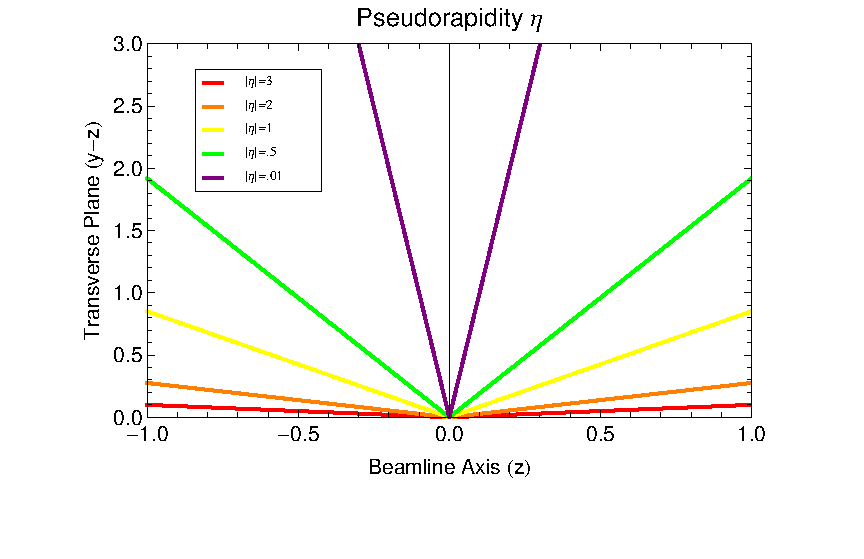
\includegraphics[width=.6\textwidth]{figures/exp_proj/pseudorapidity}
\end{center}
\caption{Lines of constant pseudorapidity in the z-y plane}
\label{fig:pseudorapidity}
\end{figure}

\framebox{$\Delta R$} Given our coordinate system, $\Delta R$ is our longitudinally boost invariant notion of distance:
\begin{align*}
\Delta R = \sqrt{ (\Delta \phi)^2 + (\Delta \eta)^2}
\end{align*}
Fixed values of $\Delta R$ form a solid angle ``cone'' extending from the interaction point outward. This can be seen by using our definition of $\eta$ to convert from cylindrical coordinates to $(x,y,z)$ and consider the distance relative to the point $(\eta_0,\phi_0)$
\begin{align*}
\Delta R = \sqrt{ \left( \phi_0 - \tan^{-1} (y/x) \right )^2 + \left ( \eta_0 + \log \left( \tan \frac{\cos^{-1} (z/\sqrt{x^2+y^2})}{2} \right) \right)^2 }
\end{align*}

\begin{figure}
\begin{center}
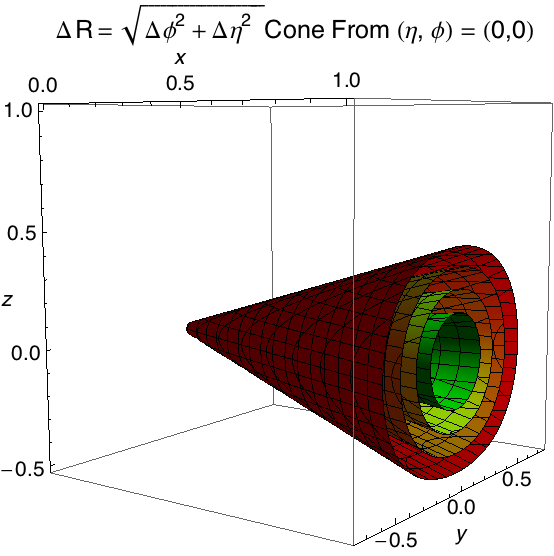
\includegraphics[width=.3\textwidth]{figures/exp_proj/deltaR_cone}
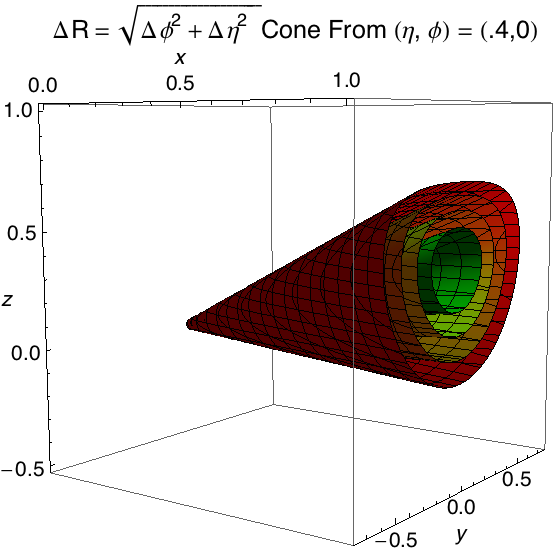
\includegraphics[width=.3\textwidth]{figures/exp_proj/deltaR_cone_eta0p4}
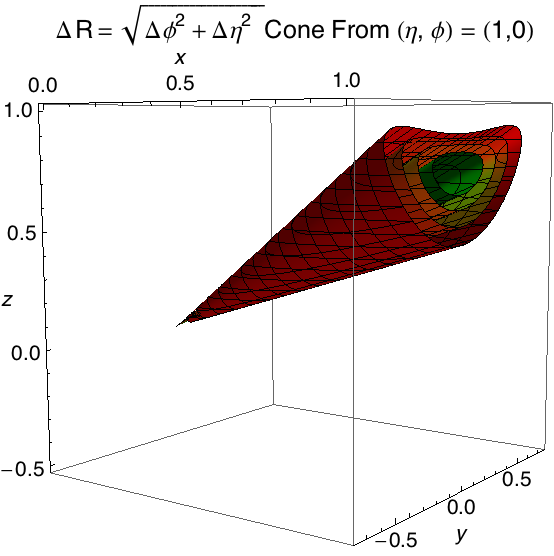
\includegraphics[width=.3\textwidth]{figures/exp_proj/deltaR_cone_eta1p0}
\end{center}
\caption{Contours of constant $\Delta R$ from the $\eta_),\phi_0 = 0,0$}
\label{fig:deltaRcones}
\end{figure}

\section{An inclusive displaced-jet tagger}

\section{Event selection}


A signal is searched for by applying the selection described in
section~\ref{sec:tagger} and counting the number of tagged displaced
jets, $N_{\textrm{tags}}$.  In addition to the online and offline
requirements described in section~\ref{sec:samples}, the analysis
signal region requires $N_{\textrm{tags}} \geq 2$.  Efficiencies are
reported for all interpreted models as a function of the lifetime with
fixed mass (Table \ref{tab:cutflow_300gev} and
\ref{tab:cutflow_BR_lifetime}) as well as a function of mass with
fixed lifetime (Table \ref{tab:cutflow_30mm} and
\ref{tab:cutflow_BR_mass}).

The two classes of events: (i) events passing the inclusive trigger
algorithm and with $H_{\textrm{T}}>650$~GeV; (ii) events passing the
exclusive trigger algorithm and with $H_{\textrm{T}}>450$~GeV are
treated as a single class.  


\begin{table}[tb]
\begin{center}
  \caption{ Signal efficiency for fixed $m_{X}=m_{\tilde{t}}=$~300~GeV
    and varied $c\tau_0$ for the Jet-Jet and B-Lepton models. Selection requirements are cumulative from
    the first to the last row. \label{tab:cutflow_300gev}}
\begin{tabular}{ccccc} 
 \multicolumn{5}{c}{\textbf{Jet-Jet}} \\
 \hline 
 $m_{X}$~[GeV] & 300 & 300 & 300 & 300 \\ 
 $c\tau_0$ [mm] & 1 & 10 & 100 & 1000 \\ 
 \hline 
 $\geq 2$ tags & 2.33 $\pm$ 0.15\% & 39.49 $\pm$ 0.63\% & 54.54 $\pm$ 0.74\% & 14.58 $\pm$ 0.38\% \\ 
 Trigger & 2.16 $\pm$ 0.15\% & 38.12 $\pm$ 0.62\% & 39.32 $\pm$ 0.63\% & 8.07 $\pm$ 0.28\% \\ 
 Event sel.& 2.09 $\pm$ 0.14\% & 37.09 $\pm$ 0.61\% & 36.53 $\pm$ 0.60\% & 6.67 $\pm$ 0.26\% \\ 
 $\geq 3$ tags &       0.170 $\pm$ 0.041\% &       14.14 $\pm$ 0.38\% &   16.72 $\pm$ 0.41\% &    1.36 $\pm$ 0.12\% \\  
 $\geq 4$ tags &       0.010 $\pm$ 0.010\% &       4.73 $\pm$ 0.22\% &    4.71 $\pm$ 0.22\% &     0.170 $\pm$ 0.041\% \\
\end{tabular}
\end{center}

\begin{center}
\begin{tabular}{ccccc} 
\multicolumn{5}{c}{\textbf{B-Lepton}} \\
 \hline 
$m_{\tilde{t}}$~[GeV] & 300 & 300 & 300 & 300 \\ 
$c\tau_0$ [mm] & 1 & 10 & 100 & 1000 \\ 
\hline 
$\geq 2$ tags &        0.453 $\pm$ 0.023\% &   15.82 $\pm$ 0.13\% &    31.52 $\pm$ 0.19\% &    8.545 $\pm$ 0.098\% \\ 
Trigger &     0.291 $\pm$ 0.018\% &        11.45 $\pm$ 0.11\% &   17.08 $\pm$ 0.14\% &    3.224 $\pm$ 0.060\% \\ 
Event sel. &   0.269 $\pm$ 0.017\% &  9.91 $\pm$ 0.11\% &    13.33 $\pm$ 0.12\% &    2.084 $\pm$ 0.048\% \\ 
$\geq 3$ tags &     0.017 $\pm$ 0.004\% &  2.462 $\pm$ 0.053\% &  3.814 $\pm$ 0.065\% &   0.368 $\pm$ 0.020\% \\ 
$\geq 4$ tags &      -- &      0.297 $\pm$ 0.018\% &  0.480 $\pm$ 0.023\% &   0.0315 $\pm$ 0.0060\% \\ 
\end{tabular}
\end{center}
\end{table}

\begin{table}[tb]
  \caption{ Signal efficiency for fixed $m_{X}=m_{\tilde{t}}=300$~GeV
    and varied $c\tau_0$ with modified branching ratios relative to 
    the Jet-Jet and B-Lepton models. Selection requirements are cumulative from
    the first to the last row.  
    \label{tab:cutflow_BR_lifetime}}
\begin{center}
\begin{tabular}{ccccc} 
\multicolumn{5}{c}{\textbf{Light-Light}} \\
 \hline 
 $m_{X}$~[GeV] & 300 & 300 & 300 & 300 \\ 
 $c\tau_0$ [mm] & 1 & 10 & 100 & 1000 \\ 
 \hline 
 $\geq 2$ tags &        2.20 $\pm$ 0.19\% &     40.49 $\pm$ 0.80\% &    54.92 $\pm$ 0.93\% &    14.55 $\pm$ 0.47\% \\ 
 Trigger &     2.04 $\pm$ 0.18\% &        39.16 $\pm$ 0.78\% &     39.63 $\pm$ 0.79\% &    8.20 $\pm$ 0.36\% \\ 
 Event sel. &  2.03 $\pm$ 0.18\% &   38.41 $\pm$ 0.77\% &     36.99 $\pm$ 0.76\% &    6.89 $\pm$ 0.33\% \\ 
 $\geq 3$ tags &    0.187 $\pm$ 0.054\% &       14.77 $\pm$ 0.48\% &     16.70 $\pm$ 0.51\% &   1.48 $\pm$ 0.15\% \\ 
 $\geq 4$ tags &    -- &     5.11 $\pm$ 0.28\% &   4.73 $\pm$ 0.27\% &      0.216 $\pm$ 0.058\% \\ 
\end{tabular}

\begin{tabular}{ccccc} 
\multicolumn{5}{c}{\textbf{B-Ele}} \\
 \hline 
 $m_{\tilde{t}}$~[GeV] & 300 & 300 & 300 & 300 \\ 
 $c\tau_0$ [mm] & 1 & 10 & 100 & 1000 \\ 
 \hline 
  $\geq 2$ tags &        0.807 $\pm$ 0.093\% &   20.51 $\pm$ 0.47\% &    39.01 $\pm$ 0.65\% &    11.46 $\pm$ 0.35\% \\ 
   Trigger &     0.398 $\pm$ 0.065\% &        14.68 $\pm$ 0.40\% &   22.95 $\pm$ 0.50\% &    5.15 $\pm$ 0.23\% \\ 
    Event sel. &   0.398 $\pm$ 0.065\% &  13.92 $\pm$ 0.39\% &   20.34 $\pm$ 0.47\% &    3.58 $\pm$ 0.19\% \\ 
     $\geq 3$ tags &     0.043 $\pm$ 0.022\% &  4.22 $\pm$ 0.21\% &    7.21 $\pm$ 0.28\% &     0.822 $\pm$ 0.093\% \\ 
      $\geq 4$ tags &     -- &  0.727 $\pm$ 0.088\% &       1.19 $\pm$ 0.11\% &    0.053 $\pm$ 0.024\% \\ 
\end{tabular}

\begin{tabular}{ccccc} 
\multicolumn{5}{c}{\textbf{B-Tau}} \\
 \hline 
$m_{\tilde{t}}$~[GeV] & 300 & 300 & 300 & 300 \\ 
 $c\tau_0$ [mm] & 1 & 10 & 100 & 1000 \\ 
\hline 
$\geq 2$ tags &  0.483 $\pm$ 0.073\% &   18.40 $\pm$ 0.45\% &    34.98 $\pm$ 0.61\% &    9.31 $\pm$ 0.32\% \\ 
Trigger &     0.439 $\pm$ 0.069\% &  14.63 $\pm$ 0.40\% &   20.20 $\pm$ 0.46\% &    3.81 $\pm$ 0.20\% \\ 
Event sel. &   0.406 $\pm$ 0.067\% &  12.45 $\pm$ 0.37\% &   15.50 $\pm$ 0.41\% &   2.37 $\pm$ 0.16\% \\ 
$\geq 3$ tags &     0.022 $\pm$ 0.016\% &  3.23 $\pm$ 0.19\% &    4.62 $\pm$ 0.22\% &    0.441 $\pm$ 0.069\% \\ 
$\geq 4$ tags &     -- &  0.525 $\pm$ 0.076\% &       0.660 $\pm$ 0.084\% &  0.022 $\pm$ 0.015\% \\ 
\end{tabular}

\begin{tabular}{ccccc} 
\multicolumn{5}{c}{\textbf{B-Mu}} \\
 \hline 
 $m_{\tilde{t}}$~[GeV] & 300 & 300 & 300 & 300 \\ 
 $c\tau_0$ [mm] & 1 & 10 & 100 & 1000 \\ 
 \hline 
  $\geq 2$ tags &        0.130 $\pm$ 0.037\% &   8.02 $\pm$ 0.29\% &     20.09 $\pm$ 0.46\% &    4.03 $\pm$ 0.21\% \\ 
   Trigger &     0.054 $\pm$ 0.024\% &        3.97 $\pm$ 0.21\% &   6.63 $\pm$ 0.26\% &      0.881 $\pm$ 0.098\% \\ 
    Event sel. &   0.043 $\pm$ 0.022\% &  2.92 $\pm$ 0.18\% &   4.21 $\pm$ 0.21\% &      0.489 $\pm$ 0.073\% \\ 
     $\geq 3$ tags &     -- &  0.227 $\pm$ 0.049\% &       0.307 $\pm$ 0.057\% &        0.033 $\pm$ 0.019\% \\ 
      $\geq 4$ tags &     -- &  0.011 $\pm$ 0.011\% &       -- &  -- \\ 
\end{tabular}
\end{center}
\end{table}

\begin{table}[tb]
\begin{center}
  \caption{ Signal efficiencies for the Jet-Jet and B-Lepton models
    with $c\tau_0=$~30mm and varied mass. Selection requirements are cumulative from
    the first to the last row. \label{tab:cutflow_30mm}}
\begin{tabular}{ccccc}
\multicolumn{5}{c}{\textbf{Jet-Jet}} \\
 \hline 
 $m_{X}$~[GeV] & 50 & 100 & 300 & 1000  \\ 
 $c\tau_0$ [mm] & 30 & 30 & 30 & 30  \\ 
 \hline 
 $\geq 2$ tags &        2.710 $\pm$ 0.095\% &   14.80 $\pm$ 0.22\% &    54.24 $\pm$ 0.74\% &    79.93 $\pm$ 0.89\%  \\ 
 Trigger &     0.503 $\pm$ 0.041\% &        5.39 $\pm$ 0.13\% &    46.41 $\pm$ 0.68\% &    74.05 $\pm$ 0.86\%\\ 
 Event sel. &   0.297 $\pm$ 0.031\% &  3.70 $\pm$ 0.11\% &    44.75 $\pm$ 0.67\% &    73.99 $\pm$ 0.86\%\\ 
 $\geq 3$ tags &     0.050 $\pm$ 0.013\% &  1.087 $\pm$ 0.060\% &  20.87 $\pm$ 0.46\% &    49.42 $\pm$ 0.70\%\\ 
 $\geq 4$ tags &     -- &  0.217 $\pm$ 0.027\% &  6.81 $\pm$ 0.26\% &    25.45 $\pm$ 0.50\%  \\ 
\\
\end{tabular}
\begin{tabular}{ccccc}
\multicolumn{5}{c}{\textbf{B-Lepton}}\\
\hline
 $m_{\tilde{t}}$~[GeV] & 300 & 600 & 800 & 1000 \\
 $c\tau_0$ [mm] & 30 & 30 & 30 & 30 \\
 \hline
 $\geq 2$ tags &        31.52 $\pm$ 0.19\% &    47.32 $\pm$ 0.23\% &    52.53 $\pm$ 0.24\% &    55.88 $\pm$ 0.35\% \\ 
Trigger &     17.08 $\pm$ 0.14\% &        35.03 $\pm$ 0.20\% &    40.40 $\pm$ 0.21\% &    43.14 $\pm$ 0.30\% \\ 
Event sel. &   14.70 $\pm$ 0.13\% &  32.34 $\pm$ 0.19\% &    36.94 $\pm$ 0.20\% &    39.26 $\pm$ 0.29\% \\ 
$\geq 3$ tags &     4.106 $\pm$ 0.068\% &       10.76 $\pm$ 0.11\% &    13.29 $\pm$ 0.12\% &    15.00 $\pm$ 0.18\% \\ 
$\geq 4$ tags &     0.552 $\pm$ 0.025\% &       1.828 $\pm$ 0.045\% &   2.687 $\pm$ 0.055\% &   3.092 $\pm$ 0.082\% \\ 
\end{tabular}
\end{center}
\end{table}

\begin{table}[tb]
  \caption{ Signal efficiency for fixed  $c\tau_0=30$mm and
   varied mass with modified branching ratios relative 
   to the Jet-Jet and B-Lepton models. Selection requirements are cumulative from
    the first to the last row.\label{tab:cutflow_BR_mass}}
\begin{center}
\begin{tabular}{cccccc} 
\multicolumn{6}{c}{\textbf{Light-Light}} \\
 \hline 
 $m_{X}$~[GeV] & 50 & 100 & 300 & 1000  \\ 
 $c\tau_0$ [mm] & 30 & 30 & 30 & 30 &  \\ 
 \hline 
 $\geq 2$ tags &        2.84 $\pm$ 0.12\% &     15.56 $\pm$ 0.29\% &    54.87 $\pm$ 0.92\% &    80.52 $\pm$ 1.11\%     \\ 
 Trigger &     0.530 $\pm$ 0.052\% &      5.70 $\pm$ 0.17\% &      47.14 $\pm$ 0.85\% &    74.85 $\pm$ 1.07\%\\ 
 Event sel. &   0.327 $\pm$ 0.041\% &     3.90 $\pm$ 0.14\% &       45.68 $\pm$ 0.84\% &    74.80 $\pm$ 1.07\%\\ 
 $\geq 3$ tags &     0.052 $\pm$ 0.016\% &     1.113 $\pm$ 0.076\% &     21.77 $\pm$ 0.58\% &    50.04 $\pm$ 0.88\%\\ 
 $\geq 4$ tags &     -- &  0.230 $\pm$ 0.035\% &     7.38 $\pm$ 0.34\% &       25.80 $\pm$ 0.63\% &    \\ 
\end{tabular}

\begin{tabular}{ccccc} 
\multicolumn{5}{c}{\textbf{B-Ele}} \\
 \hline 
 $m_{\tilde{t}}$~[GeV] & 300 & 600 & 800 & 1000 \\ 
 $c\tau_0$ [mm] & 30 & 30 & 30 & 30 \\ 
\hline 
        $\geq 2$ tags &  39.01 $\pm$ 0.65\% &    53.70 $\pm$ 0.75\% &    59.62 $\pm$ 0.78\% &    62.42 $\pm$ 1.11\% \\ 
         Trigger &     22.95 $\pm$ 0.50\% &  38.07 $\pm$ 0.63\% &    43.06 $\pm$ 0.66\% &    45.21 $\pm$ 0.95\% \\ 
          Event sel. &   21.59 $\pm$ 0.48\% &  37.02 $\pm$ 0.62\% &    39.47 $\pm$ 0.64\% &    42.20 $\pm$ 0.92\% \\ 
           $\geq 3$ tags &     7.86 $\pm$ 0.29\% &   14.28 $\pm$ 0.38\% &    17.37 $\pm$ 0.42\% &    20.39 $\pm$ 0.64\% \\ 
            $\geq 4$ tags &     1.37 $\pm$ 0.12\% &   3.32 $\pm$ 0.19\% &     4.34 $\pm$ 0.21\% &     4.69 $\pm$ 0.31\% \\ 
\end{tabular}

\begin{tabular}{ccccc} 
\multicolumn{5}{c}{\textbf{B-Tau}} \\
 \hline 
 $m_{\tilde{t}}$~[GeV] & 300 & 600 & 800 & 1000 \\ 
$c\tau_0$ [mm] & 30 & 30 & 30 & 30 \\ 
 \hline 
$\geq 2$ tags & 34.98 $\pm$ 0.61\% & 51.42 $\pm$ 0.73\% & 57.20 $\pm$ 0.76\% & 59.43 $\pm$ 1.07\% \\ 
 Trigger & 20.20 $\pm$ 0.46\% & 39.78 $\pm$ 0.64\% & 45.46 $\pm$ 0.68\% & 47.62 $\pm$ 0.96\% \\ 
 Event sel.& 17.17 $\pm$ 0.43\% & 37.47 $\pm$ 0.62\% & 43.64 $\pm$ 0.67\% & 44.26 $\pm$ 0.92\% \\ 
 $\geq 3$ tags & 5.21 $\pm$ 0.24\% & 13.29 $\pm$ 0.37\% & 16.15 $\pm$ 0.40\% & 19.13 $\pm$ 0.61\% \\ 
 $\geq 4$ tags& 0.86 $\pm$ 0.10\% & 3.09 $\pm$ 0.18\% & 3.68 $\pm$ 0.19\% & 4.48 $\pm$ 0.29\% \\ 
\end{tabular}

\begin{tabular}{ccccc} 
\multicolumn{5}{c}{\textbf{B-Mu}} \\
 \hline 
 $m_{\tilde{t}}$~[GeV] & 300 & 600 & 800 & 1000 \\ 
 $c\tau_0$ [mm] & 30 & 30 & 30 & 30 \\ 
\hline 
$\geq 2$ tags &  20.09 $\pm$ 0.46\% &    35.46 $\pm$ 0.60\% &    41.18 $\pm$ 0.64\% &    43.13 $\pm$ 0.93\%     \\ 
Trigger &     6.63 $\pm$ 0.26\% &   24.73 $\pm$ 0.50\% &    31.85 $\pm$ 0.56\% &    34.10 $\pm$ 0.82\% \\ 
Event sel. &  5.25 $\pm$ 0.24\% &    21.40 $\pm$ 0.47\% &    27.42 $\pm$ 0.52\% &    31.18 $\pm$ 0.79\% \\ 
$\geq 3$ tags &    0.344 $\pm$ 0.060\% &  3.03 $\pm$ 0.18\% &     5.28 $\pm$ 0.23\% &     6.08 $\pm$ 0.35\% \\ 
$\geq 4$ tags &    -- &  0.122 $\pm$ 0.035\% &       0.677 $\pm$ 0.082\% &   0.68 $\pm$ 0.12\% \\ 
\end{tabular}
\end{center}
\end{table}


\section{Datasets and simulated samples}
\label{sec:samples}

Events are collected from two dedicated online selection algorithms,
designed to identify events with displaced jets.  The algorithms
consider jets clustered from energy deposits in the calorimeters,
using the FASTJET~\cite{fastjet} implementation of the
anti-\textit{k}$_{\textit{t}}$ algorithm~\cite{Cacciari:2008gp}, with
size parameter $0.4$. Jets with transverse momentum $p_{t}<60~$~GeV or
$|\eta|>2.0$ are discarded.  An inclusive trigger algorithm accepts
events when the scalar sum of the jet $p_{t}$'s, $H_{\textrm{T}}$, is
greater than $500$~GeV and at least two jets with $|\eta|<2.0$ and at
most two prompt tracks are found. Tracks are classified as prompt if
their transverse impact parameter relative to the beam line,
$IP^{\textrm{2D}}$, is less than $1$mm.  Another trigger
algorithm is used, which requires $H_{\textrm{T}}>350~$~GeV and asks
that there be two displaced jets each having at least one track with
transverse impact parameter
$IP^{\textrm{2D}}>5\sigma_{IP^{\textrm{2D}}}$,
where $\sigma_{IP^{\textrm{2D}}}$ is the uncertainty on
$IP^{\textrm{2D}}$. Samples with large $H_{\textrm{T}}$ are used to
study the performance of the online selection algorithms. 

Events are selected offline requiring at least two jets with
$p_{t}>60~$~GeV and $|\eta|<2.0$. As for the online selection, the
offline jet reconstruction is performed clustering energy deposits in
the calorimeters with the anti-\textit{k}$_{\textit{t}}$ algorithm,
with jet size parameter of $0.4$. Two classes of events are
considered: (i) events passing the inclusive trigger algorithm and
with $H_{\textrm{T}}>650~$~GeV and (ii) events passing the exclusive
trigger algorithm and with $H_{\textrm{T}}>450~$~GeV. The two classes 
of events sum to 786,002 unique events passing the event selection.  

The main source of background events originates from multijet
production. The properties of this background process are studied
using a simulated multijet sample, generated with
PYTHIA 8~\cite{Sjostrand:2007gs}. The NNPDF 2.3~\cite{NNPDF23}
parton distribution functions (PDFs) are used to model the parton
momentum distribution inside the colliding protons. The event
simulation includes the effect of multiple proton-proton collisions in
the same bunch crossing and in bunch crossing nearby in time, referred
to as pileup. Simulated samples are reweighted to match the pileup
profile observed in data.

The analysis is interpreted with a set of benchmark signal models.
The \textbf{Jet-Jet} model predicts pair-produced long-lived
scalar neutral particles $X^{0}$ \cite{ScalarX}, each decaying to two light quarks u,d,s,c, and b
with equal probability. The resonance
mass $m_X$ and proper lifetime $c\tau_0$ are scanned between
50~and~1500~GeV and between 1~and~2000mm, respectively. The
trigger efficiencies for a fixed  $m_X=300$ GeV and 
$c\tau_0 = 1, 30,$ and $1000$ mm are 30\%, 81\%, and 42\%  
 respectively. The trigger efficiencies for a fixed  $c\tau_0=30$
 mm and $m_{X} = 50, 100,$ and $1000$ GeV
 are 2\%, 14\%, and 92\%  respectively.

The \textbf{B-Lepton} model contains pair-produced long-lived top squarks
in R-parity violating models of Supersymmetry~\cite{DisplacedSUSY}. Each top squark decays
to one b quark and a lepton. The branching fractions of the
decay to the three lepton flavors are equal. The
resonance mass $m_{\tilde{t}}$ and proper lifetime $c\tau_0$ are
scanned between 300~and~1000GeV and between 1~and~1000mm,
respectively. The trigger efficiencies for a fixed mass 
$m_{\tilde{t}}=300$ GeV and $c\tau_0 = 1, 30,$ and $1000$ mm
 are 15\%, 41\%, and 23\%  respectively.
The trigger efficiencies for  $m_{\tilde{t}} = 500, 700,$ and $1000$ GeV and fixed  $c\tau_0=30$ mm are 64\%, 71\%, and 74\% respectively.

These models are also investigated with modified
branching fractions.  The \textbf{Light-Light} model is the Jet-Jet
model excluding decays to b quarks (equal decays to lighter quarks)
and the \textbf{B-Mu}, \textbf{B-Ele}, and \textbf{B-Tau} models are
derived from the B-Lepton model with 100\% branching fraction to
muons, electrons, and taus, respectively.  Leptonic tau decays are included 
in the \textbf{B-Tau} interpretation. All signal samples are
generated with PYTHIA, with the setup described above for the
multijet sample. 


\section{Background prediction}
\label{sec:bkg}

As typical multijets contain only a sub dominant fraction of real displaced tracks,
jets with a small multiplicity of tracks represent the dominant background.
As the tagging criteria utilize averages of all tracks matched to the jet, the likelihood of tagging a fake decreases exponentially with $N_\textrm{tracks}$. 

 Figure~\ref{fig:fake_rate} shows the fraction of jets that are tagged as displaced 
jets in data as a function of the number of tracks associated with the jet $N_\textrm{tracks}$.  
 This function is the misidentification rate of tagging a prompt jet as displaced (up to possible
 signal contamination)  and is interpreted as the probability  $p(N_\text{tracks})$ of being tagged. This
 parameterization allows for a representative estimation, event by event, of the probability of
 tagging multiple fake displaced jets. That is to say, an event with two high track multiplicity jets is much
 less probable than two single track jets to have 2 fake displaced-jet tags. 

To maintain the statistical independence of the events
that are used to perform the prediction and the events in the signal
region, the probabilities are measured in the full control sample of events
with $N_{\textrm{tags}}\leq 1$, while the final signal region requires
$N_{\textrm{tags}} \geq 2$. Additionally, this limits signal contamination in the probability measurement.
The control sample of $N_{\textrm{tags}}=1$ includes 1391 events. 

The size of the bias introduced by only measuring the misidentification rate in  
events with $N_\textrm{tags}\leq 1$ is quantifiable. For the nominal tag the size
of the effect of removing these events on the predicted number of
two tag events is negligible (0.4\%)
compared to the statistical uncertainty of the prediction.

\begin{figure}
\begin{center}
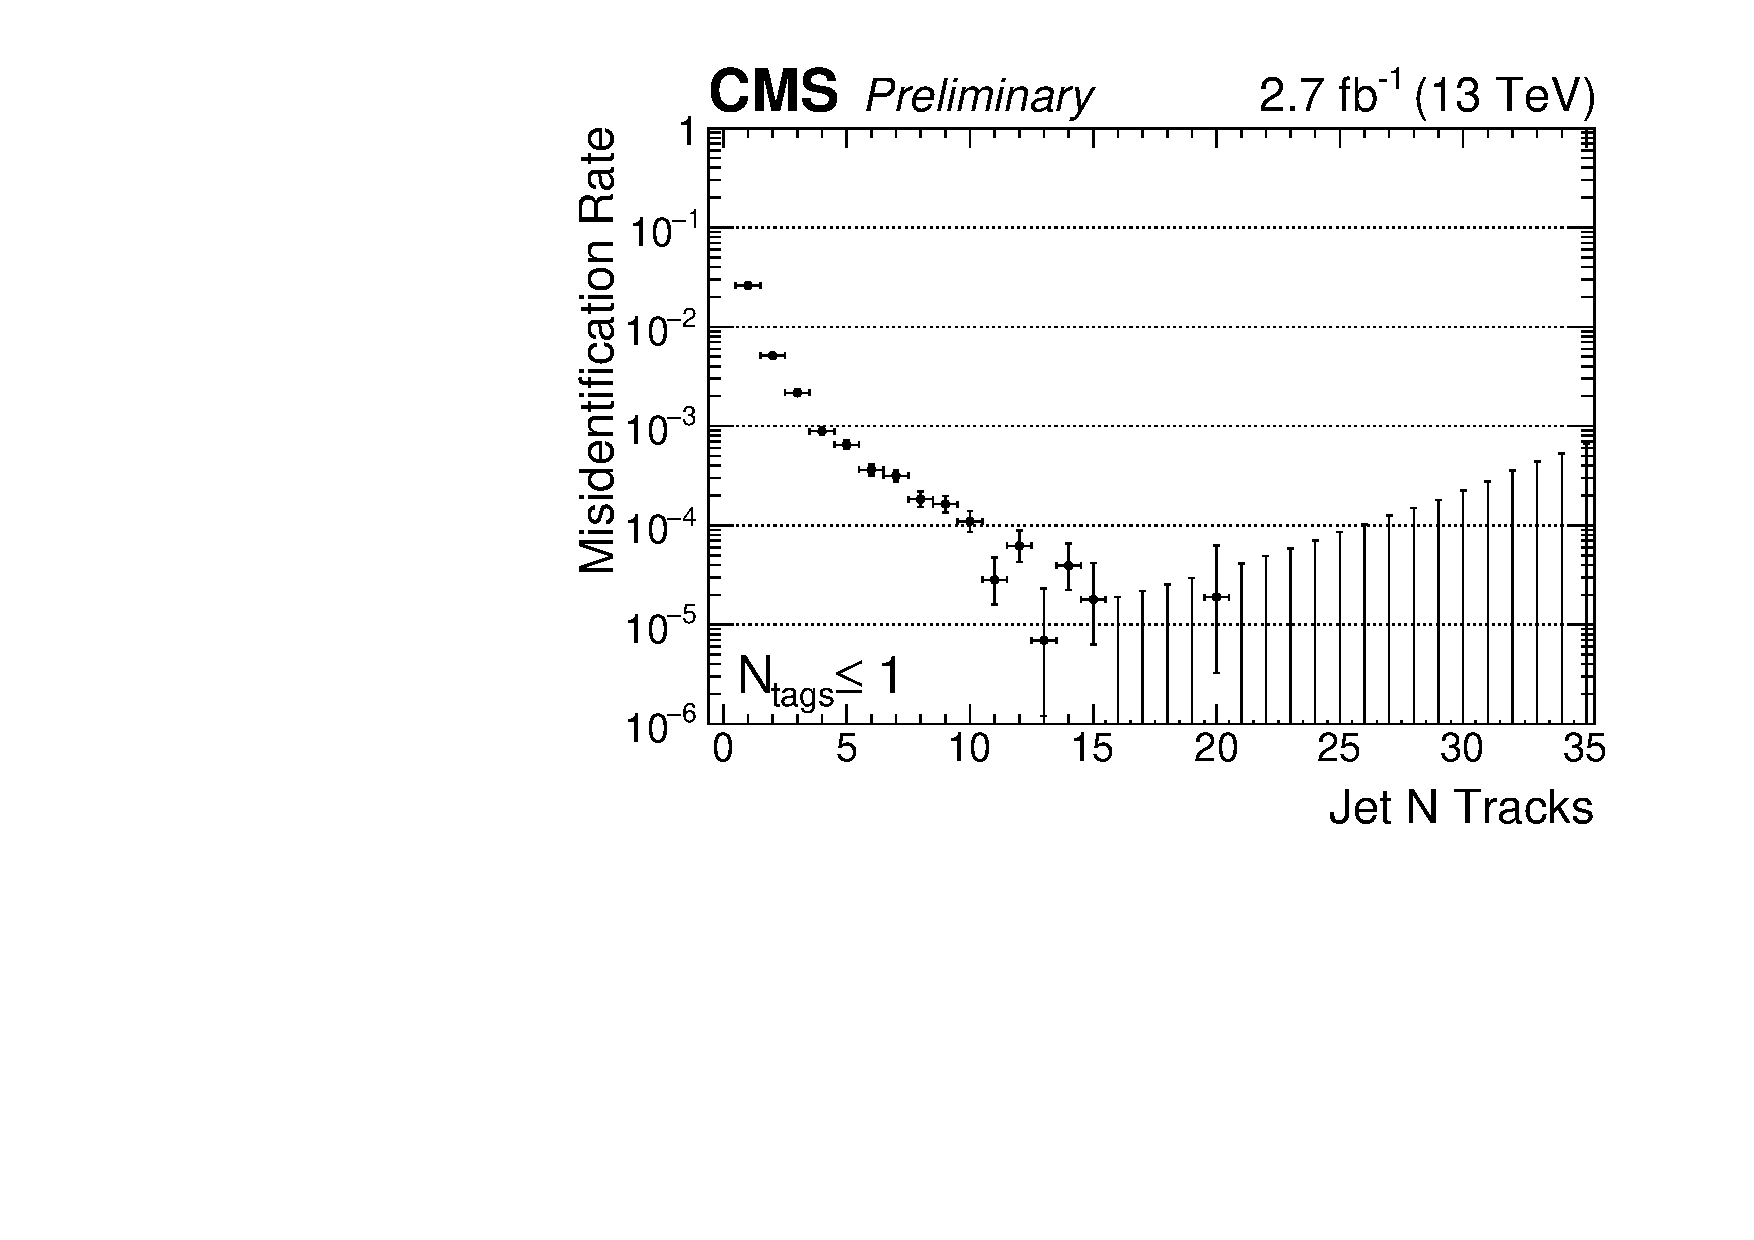
\includegraphics[width=.6\textwidth]{figures/pas//ANALYSIS/76x_pu/DJET_fakeRate.pdf}
\caption{The fraction of jets passing the displaced-jet tagging criteria as a function of the number tracks associated with the jet $N_{\textrm{tracks}}$. 
The results are from data events with $N_{\textrm{tags}} \leq 1$ collected with the displaced-jet triggers and passing the offline selection criteria. \label{fig:fake_rate}}
\end{center}
\end{figure}

The mistagging rate is used to predict the probability for an event to
have $N_\text{tags}$ tagged jets, $P(N_{\textrm{tags}})$. For instance, for an event $m$
with three jets $j_1, ~j_2$,~and~$ j_3$, there is one configuration with no tags,
with a probability:
\begin{align*} 
P^m(N_{\textrm{tags}}=0) = (1-p_1)(1-p_2)(1-p_3)~,
\end{align*} 
where $p_i = p(N_{\textrm{tracks}}(j_i))$.  Similarly, there are three
possibilities for this same event to have $N_{\textrm{tags}}=1$:
\begin{align*}
P^m(N_{\textrm{tags}}=1) = p_1(1-p_2)(1-p_3)
+  (1-p_1)p_2(1-p_3)
+  (1-p_1)(1-p_2)p_3~.
\end{align*}
The probability of finding $N_{\textrm{tags}}$  tags in the $m$ event is:
\begin{equation}
P^m(N_{\textrm{tags}}) = \sum_{\textrm{jet-configs}}~\prod_{i\in
  \textrm{tagged}} p_i \prod_{k \in \textrm{not-tagged}} (1-p_k)~.
\label{eq:ntag_prob}
\end{equation}
Tagged jets enter the product as $p_i$ and non-tagged jets enter as
$(1-p_i)$. Equation~(\ref{eq:ntag_prob}) is used to compute the
probability of observing $N_{\textrm{tags}}$, under the assumption
that the sample does not contain any signal. The number of events
expected for a given value of $N_{\textrm{tags}}$ is then computed as
\begin{equation}
N_{\textrm{events}}(N_{\textrm{tags}}) = \sum_{m} P^m(N_{\textrm{tags}})~,
\end{equation}
where $m$ runs only over events with fewer than two tagged jets.  The prediction is then compared
to the observed $N_{\textrm{tags}}$ multiplicity in events with two or
more tagged jets, to assess the presence of a signal. 

We validate this procedure in the absence (background-only test) and
presence (signal-injection test) of a signal, using simulated events.

The background-only test is performed predicting the tag multiplicity
on the simulated multijet sample, taking as input the misidentification rate
distribution. In order to populate the large-$N_{\textrm{tags}}$
region of the distribution, a looser version of the displaced-jet
tagger is employed in this test. The full sample of events passing the
event selection is divided into multiple independent samples and the background
prediction validated. The predicted background of $N_{\textrm{tags}}$ events
in simulated multijet events is found to be consistent within statistical uncertainty. 

\subsection{Signal Injection Tests} 

\subsubsection{Injection with QCD}


\begin{figure}
\begin{center}
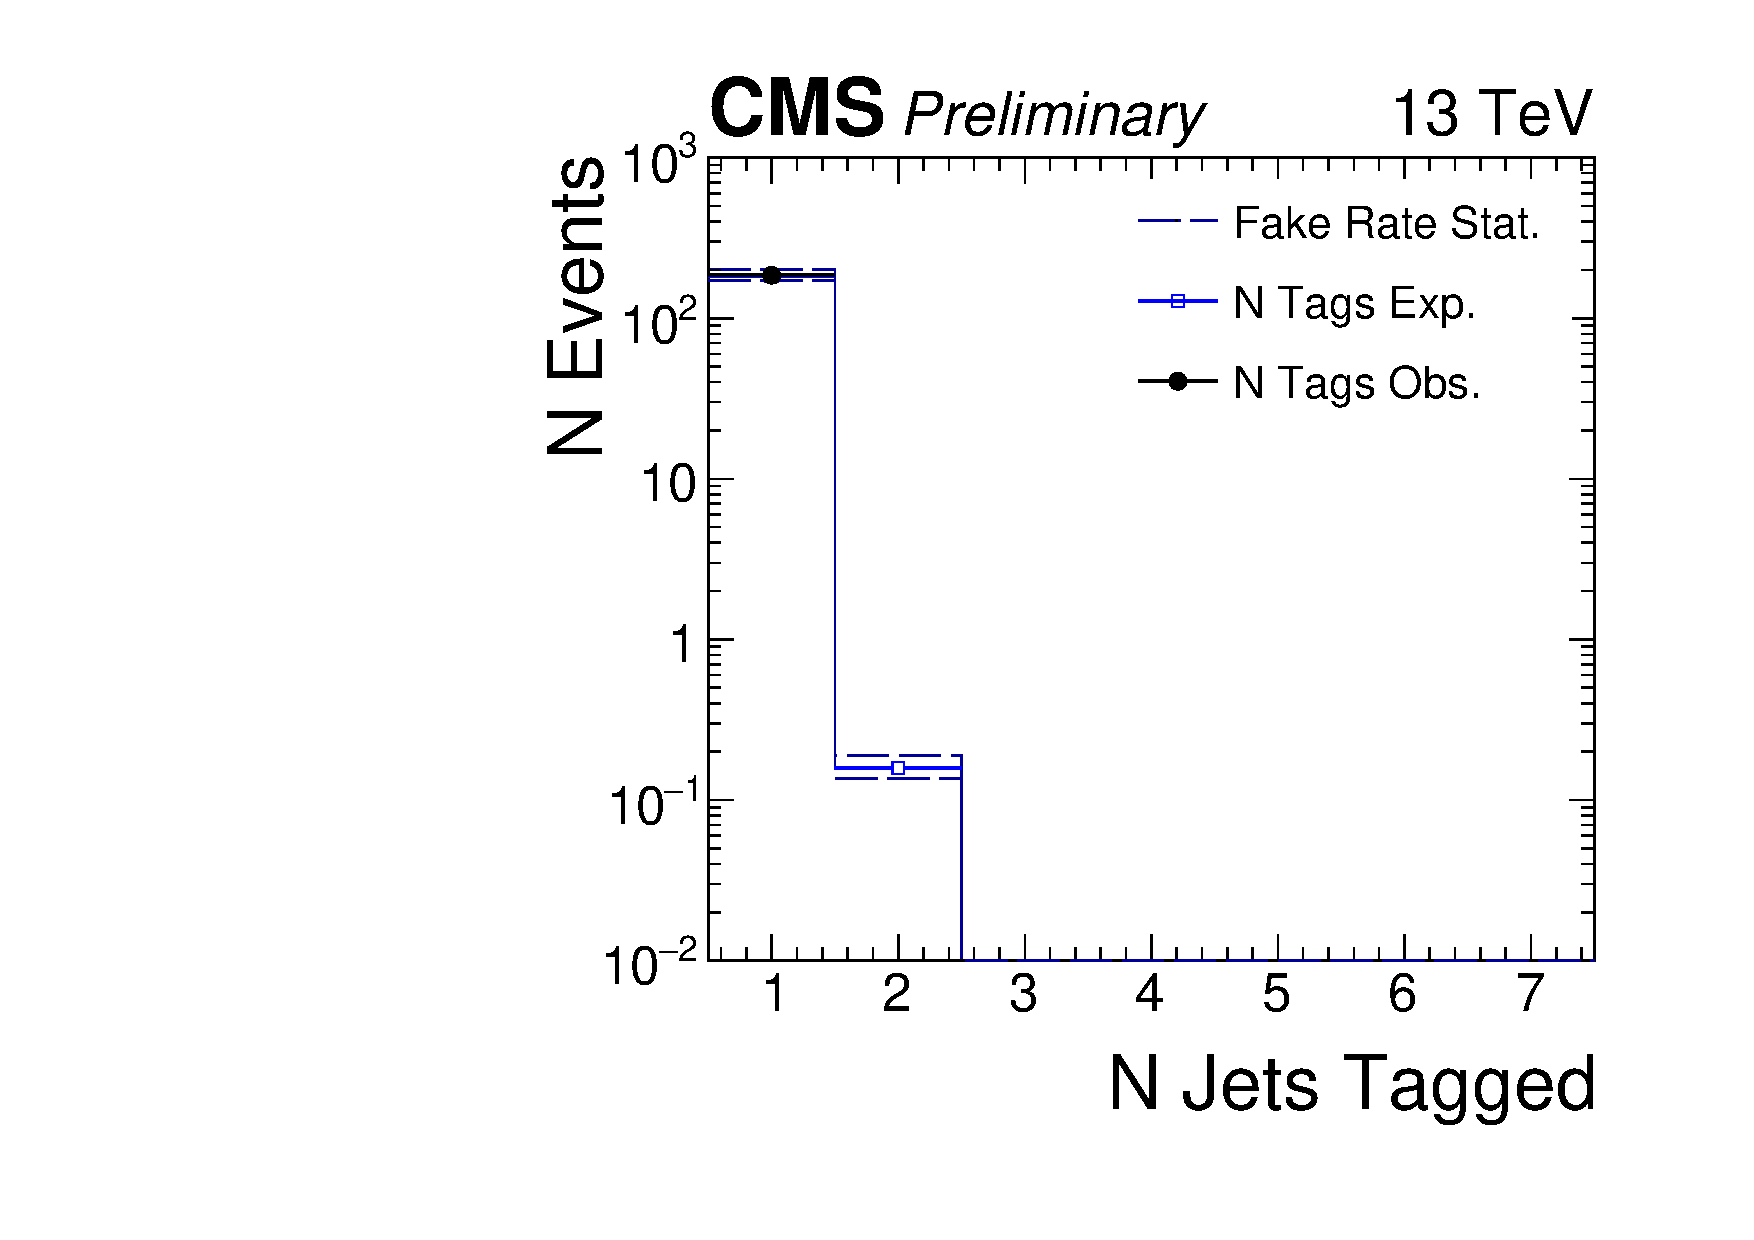
\includegraphics[width=.45\textwidth]{figures/an/ANALYSIS/76x_pu/INJECTION/qcd_loose_displacedEvtSel_0eV.pdf}\\
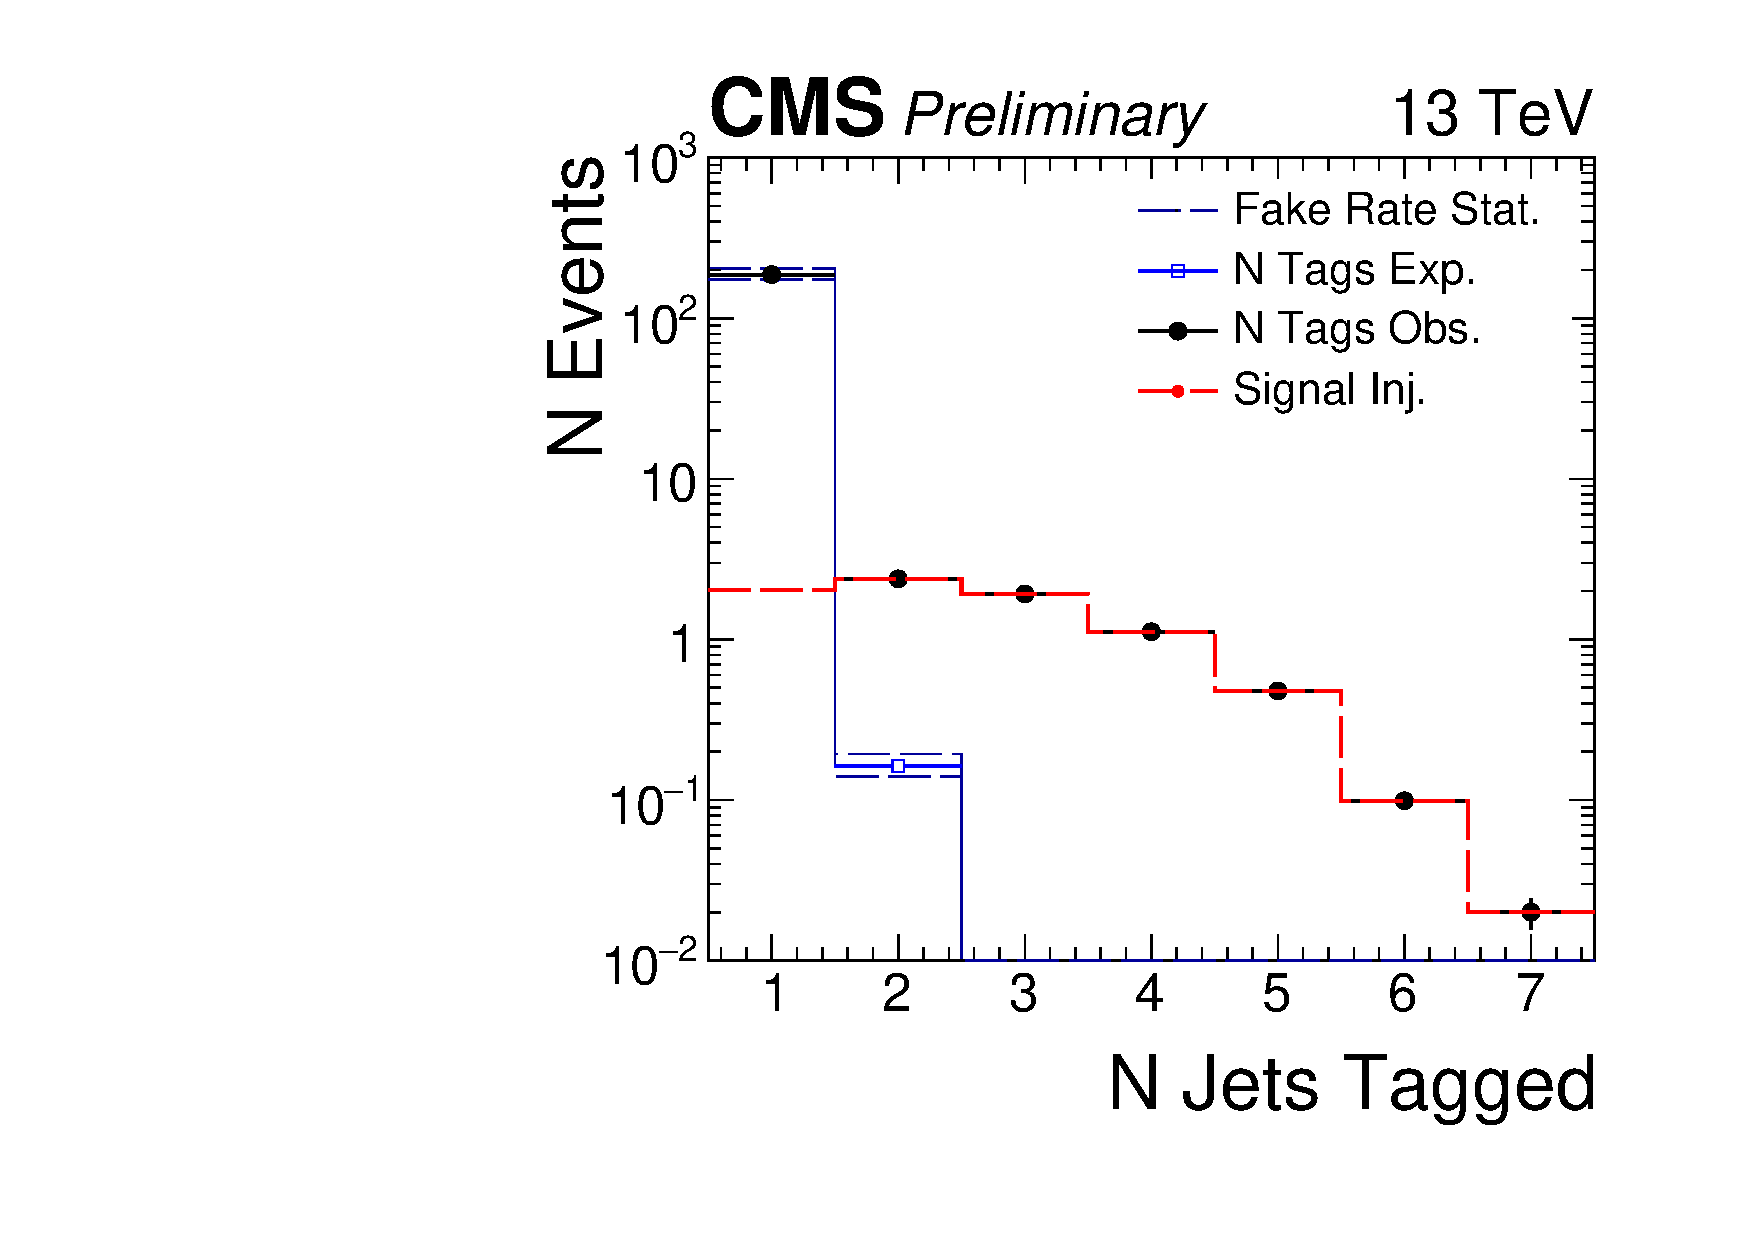
\includegraphics[width=.45\textwidth]{figures/an/ANALYSIS/76x_pu/INJECTION/qcd_loose_displacedEvtSel_10eV.pdf}
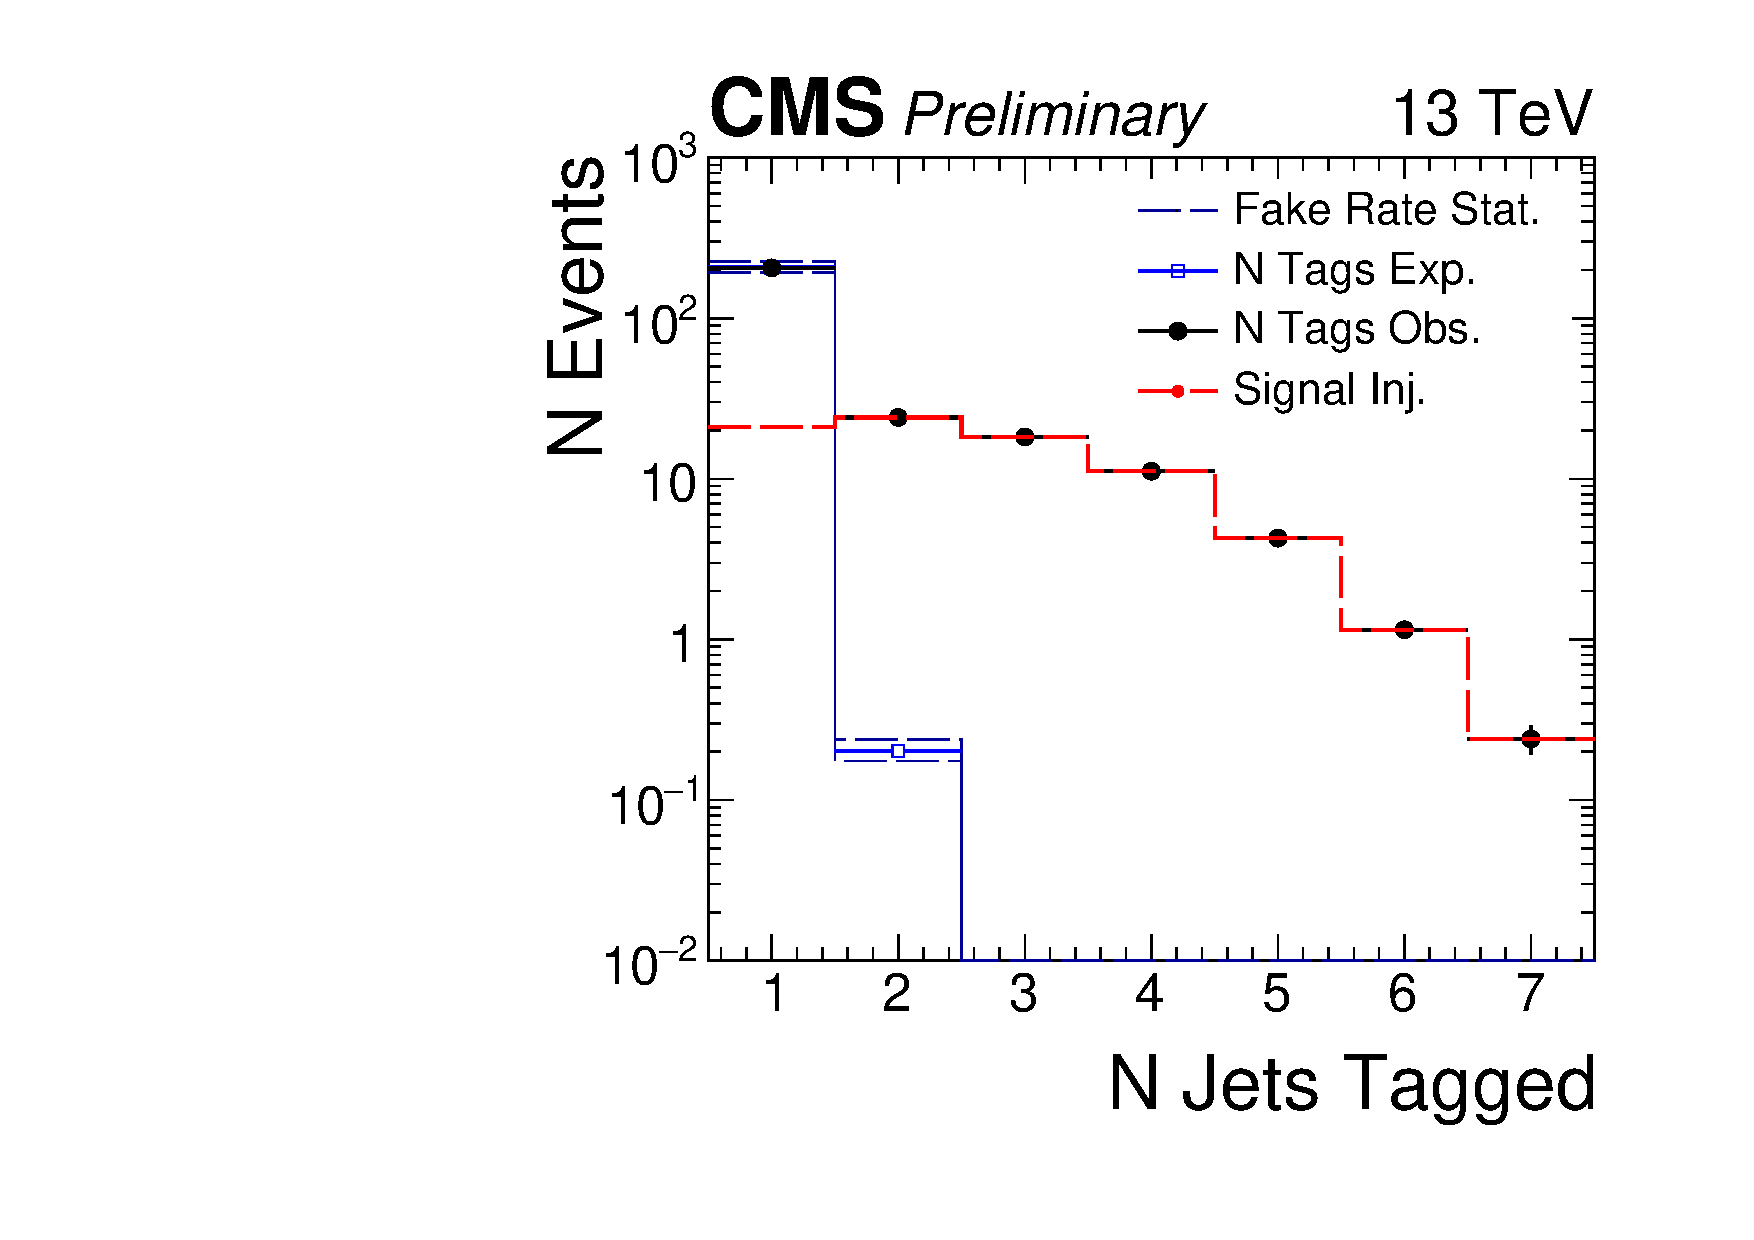
\includegraphics[width=.45\textwidth]{figures/an/ANALYSIS/76x_pu/INJECTION/qcd_loose_displacedEvtSel_100eV.pdf}\\
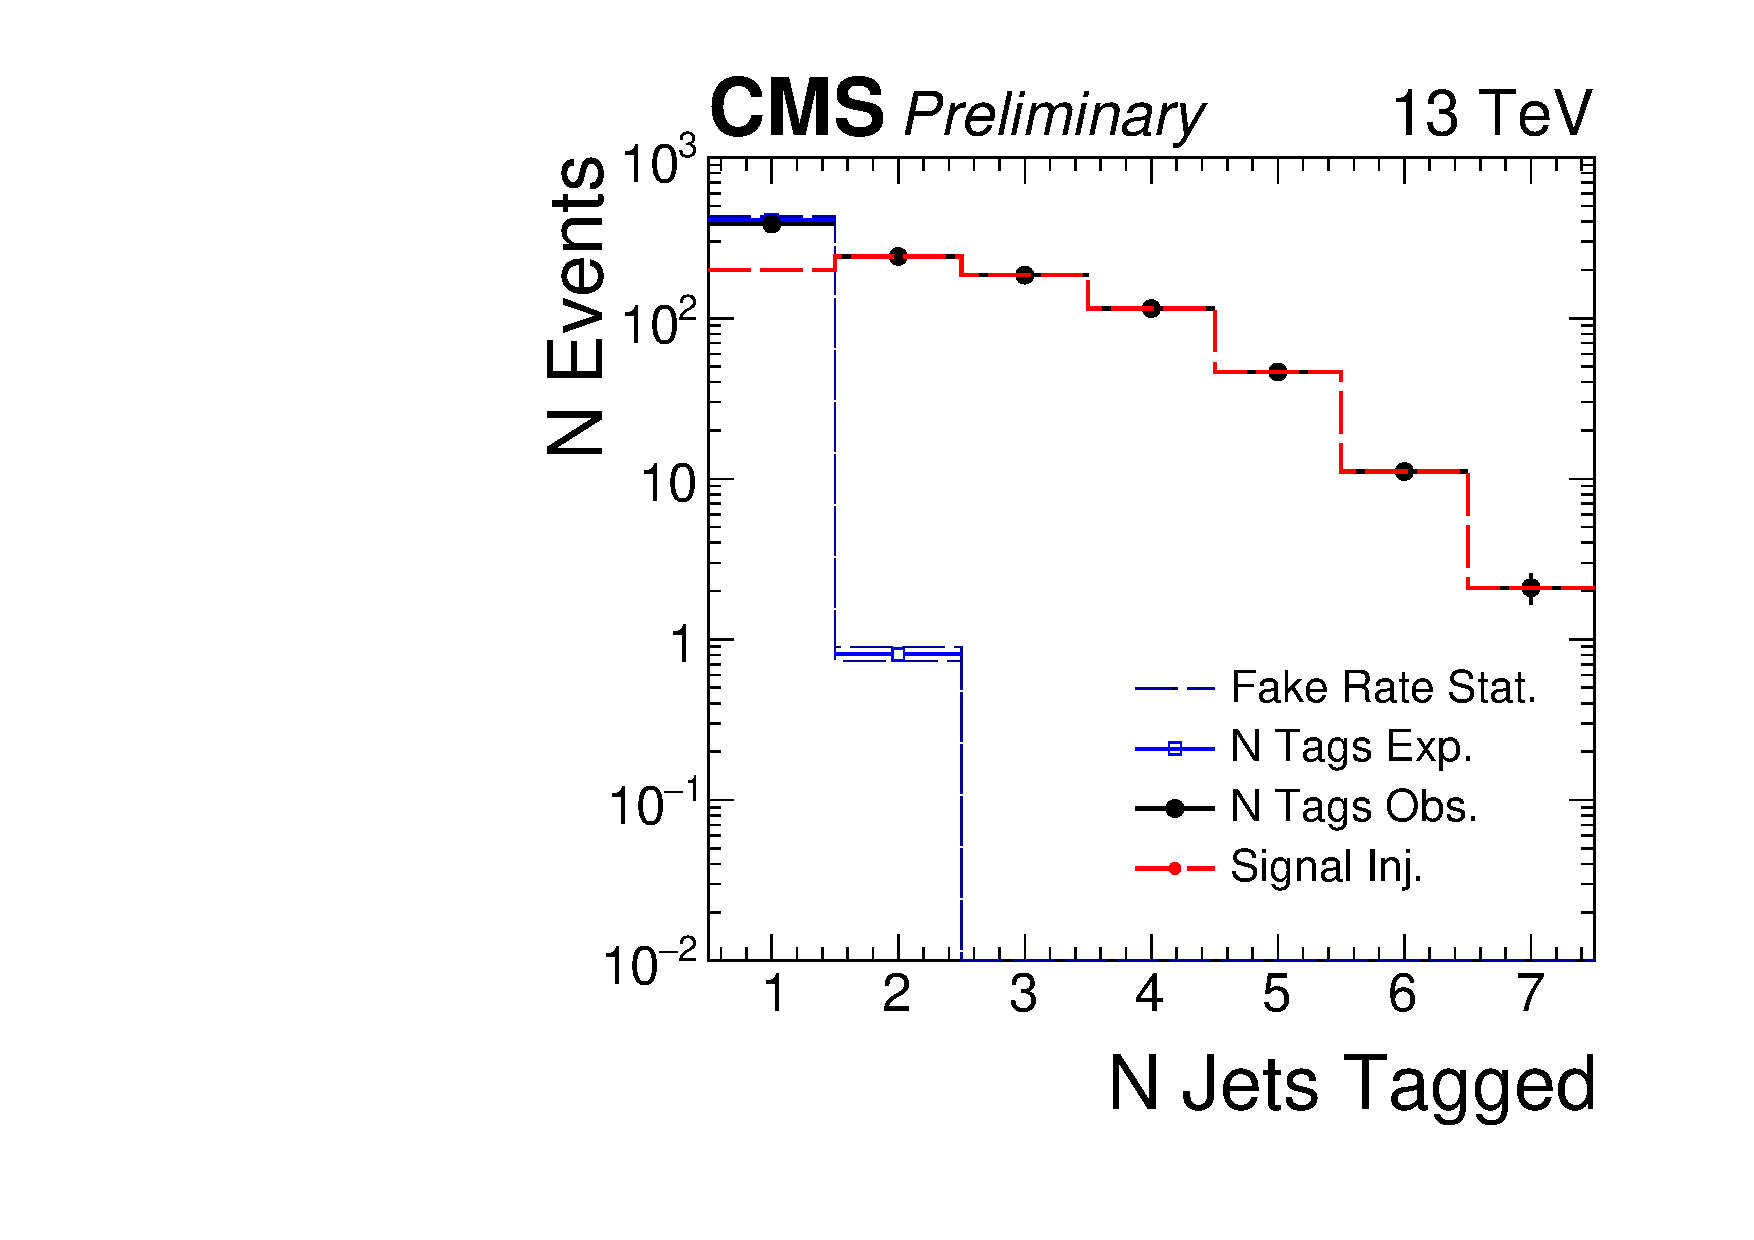
\includegraphics[width=.45\textwidth]{figures/an/ANALYSIS/76x_pu/INJECTION/qcd_loose_displacedEvtSel_1000eV.pdf}
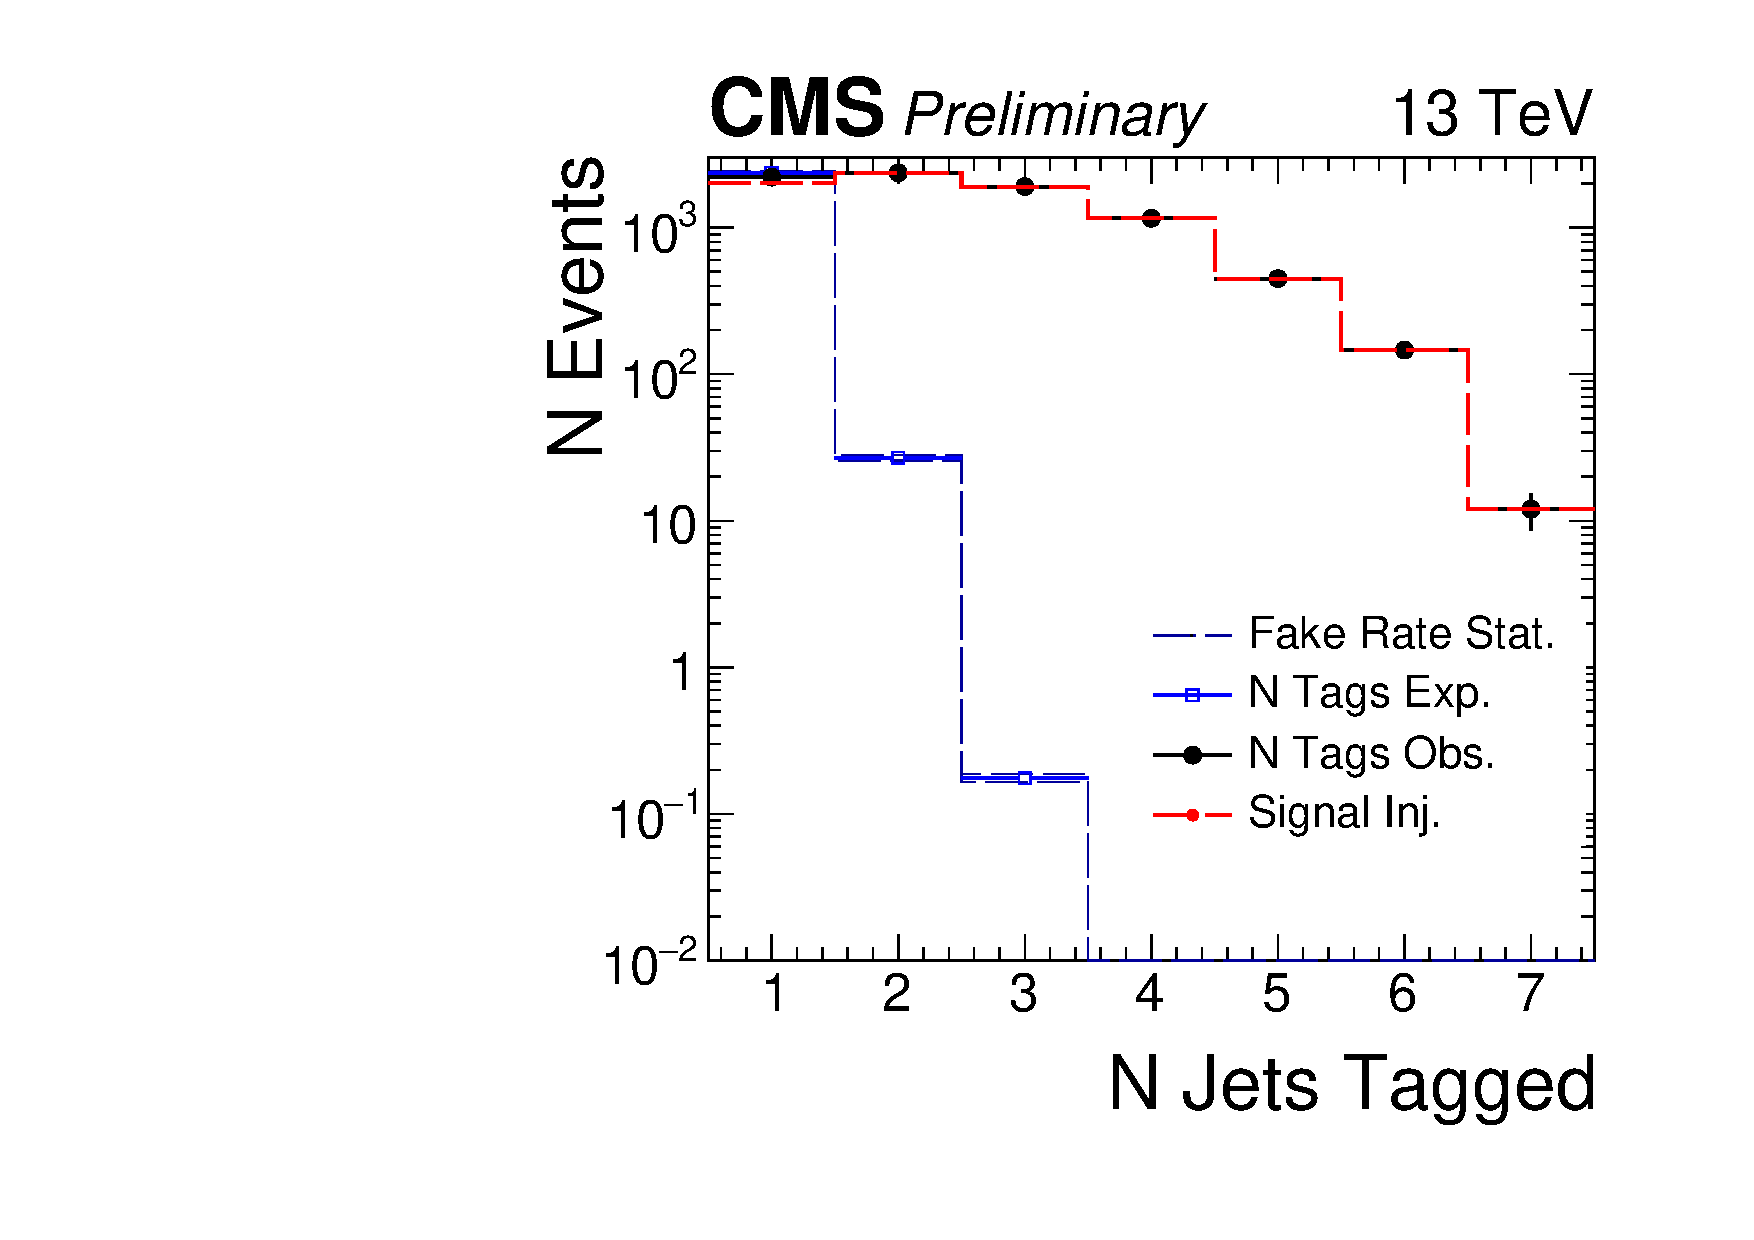
\includegraphics[width=.45\textwidth]{figures/an/ANALYSIS/76x_pu/INJECTION/qcd_loose_displacedEvtSel_10000eV.pdf}
\caption{Signal Injection tests. The Jet-Jet signal sample used has fixed $m_X=700$GeV and $c\tau_0=10$~mm. The
level of signal contamination is progressively varied between 10, 100, 1000, and 10000 events injected before any selection. The full 
event selection is applied and the baseline jet tag definition. \label{fig:injection_700_10mm}}
\end{center}
\end{figure}
\begin{figure}
\begin{center}
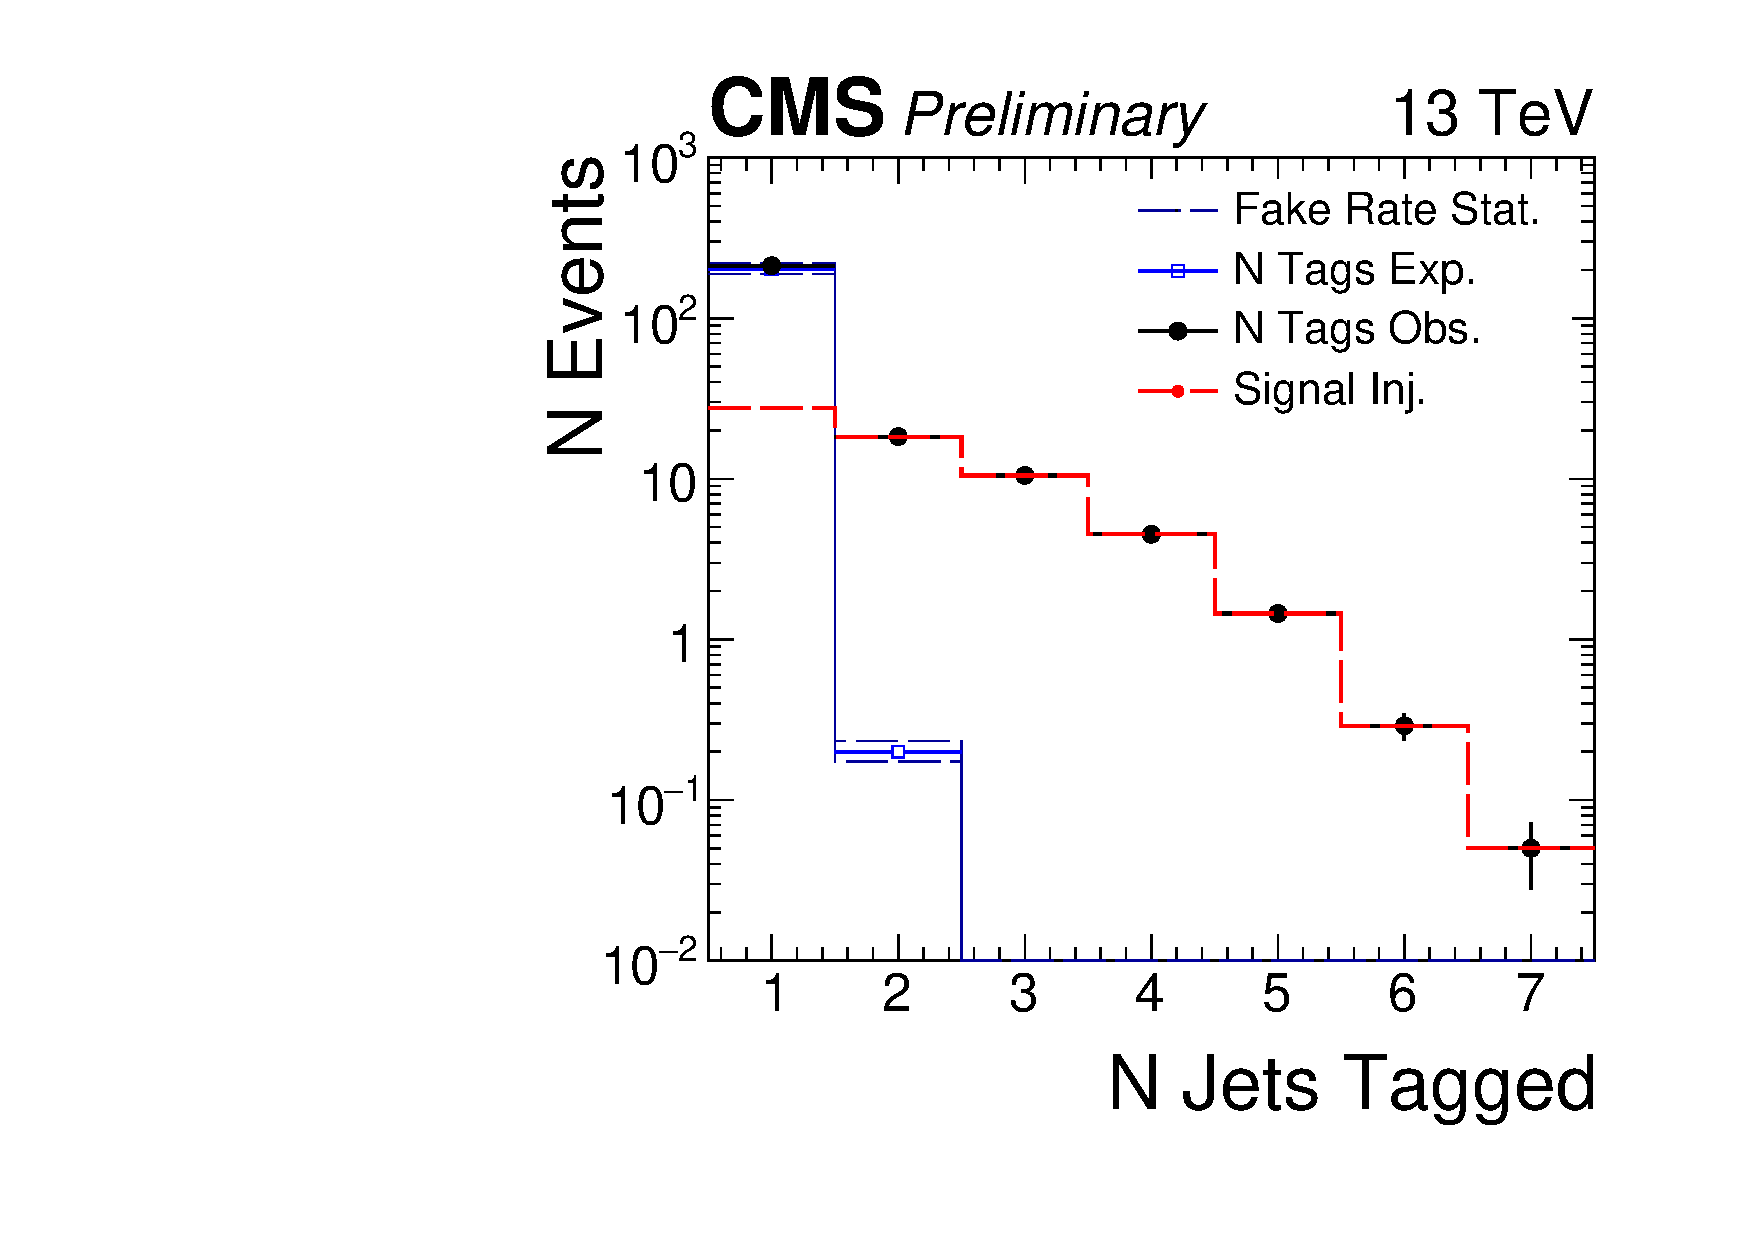
\includegraphics[width=.45\textwidth]{figures/an/ANALYSIS/76x_pu/INJECTION/mx700_ctau1000mm_100ev.pdf}
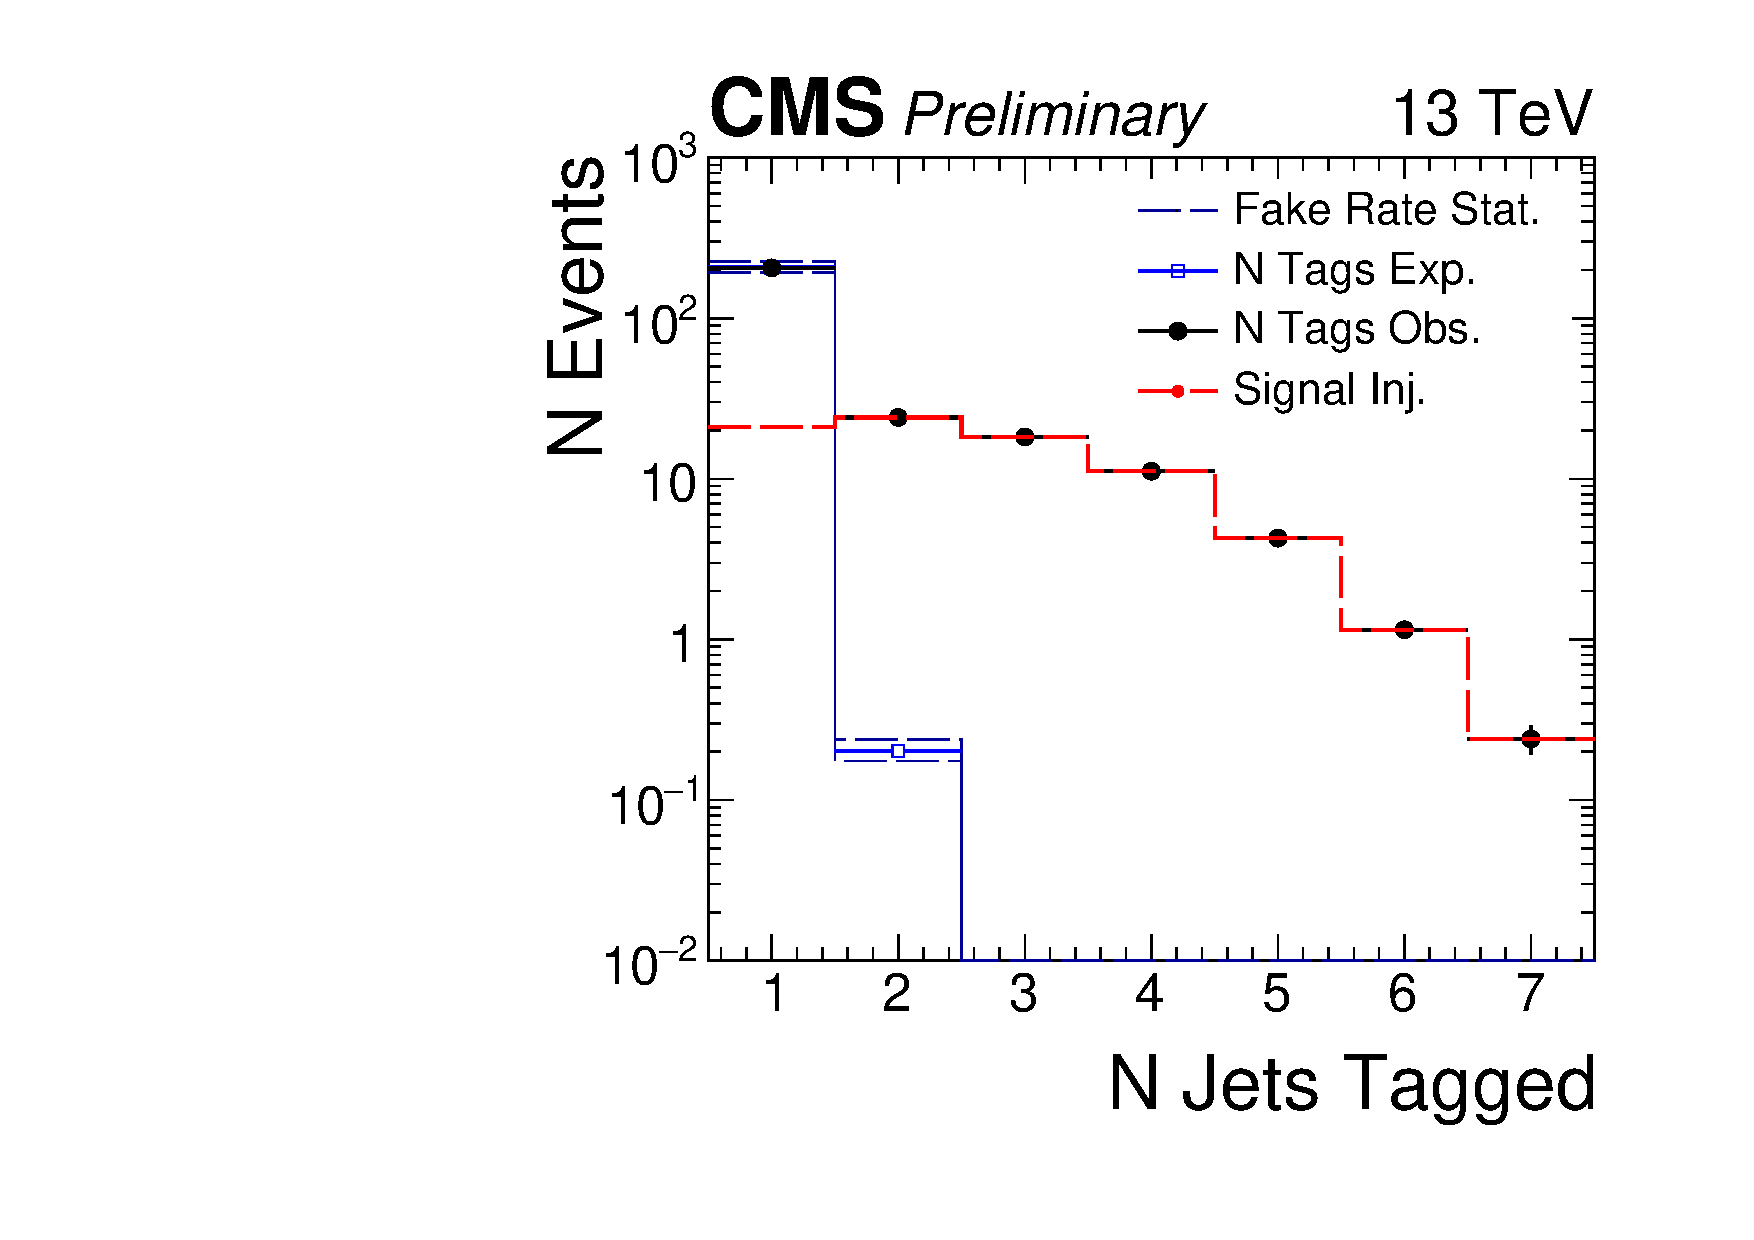
\includegraphics[width=.45\textwidth]{figures/an/ANALYSIS/76x_pu/INJECTION/qcd_loose_displacedEvtSel_100eV.pdf}\\
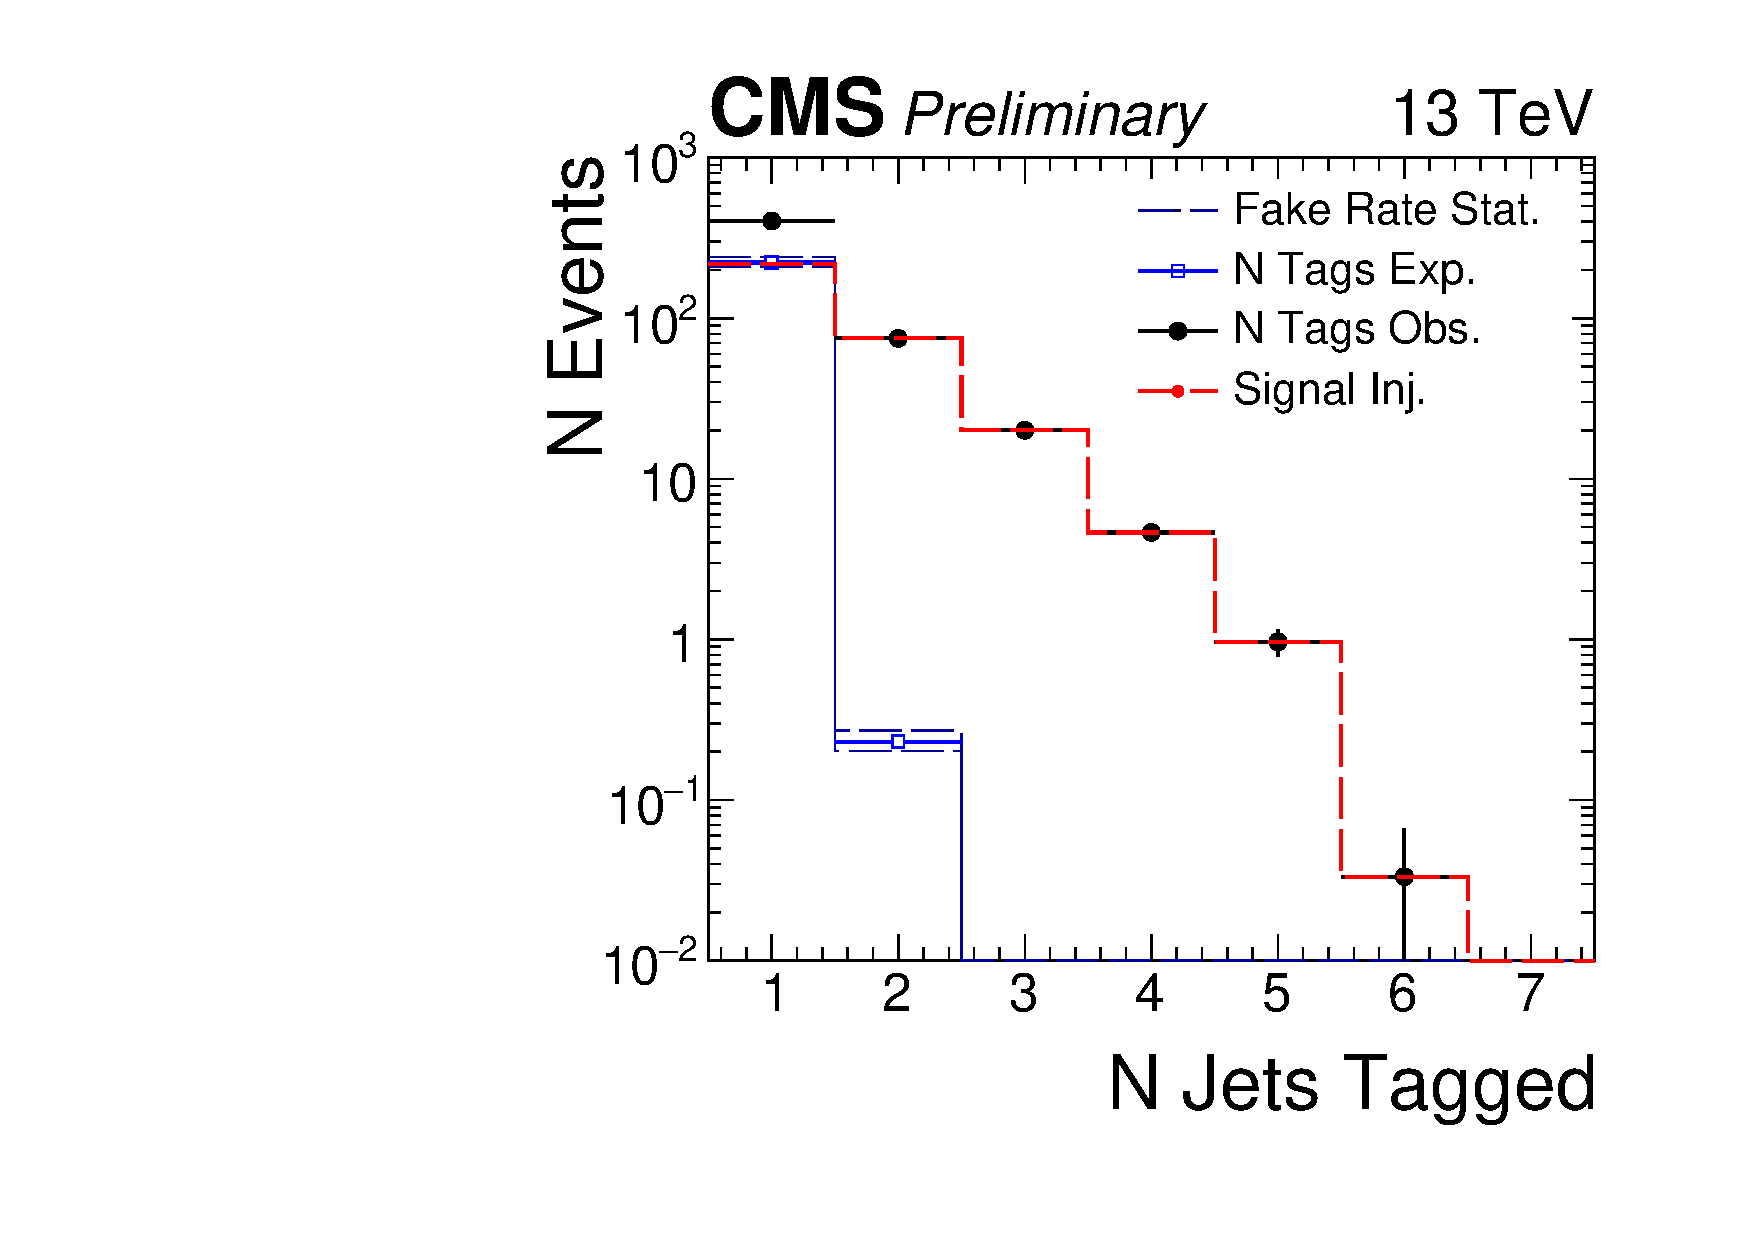
\includegraphics[width=.45\textwidth]{figures/an/ANALYSIS/76x_pu/INJECTION/mx100_ctau10mm_1000ev.pdf}
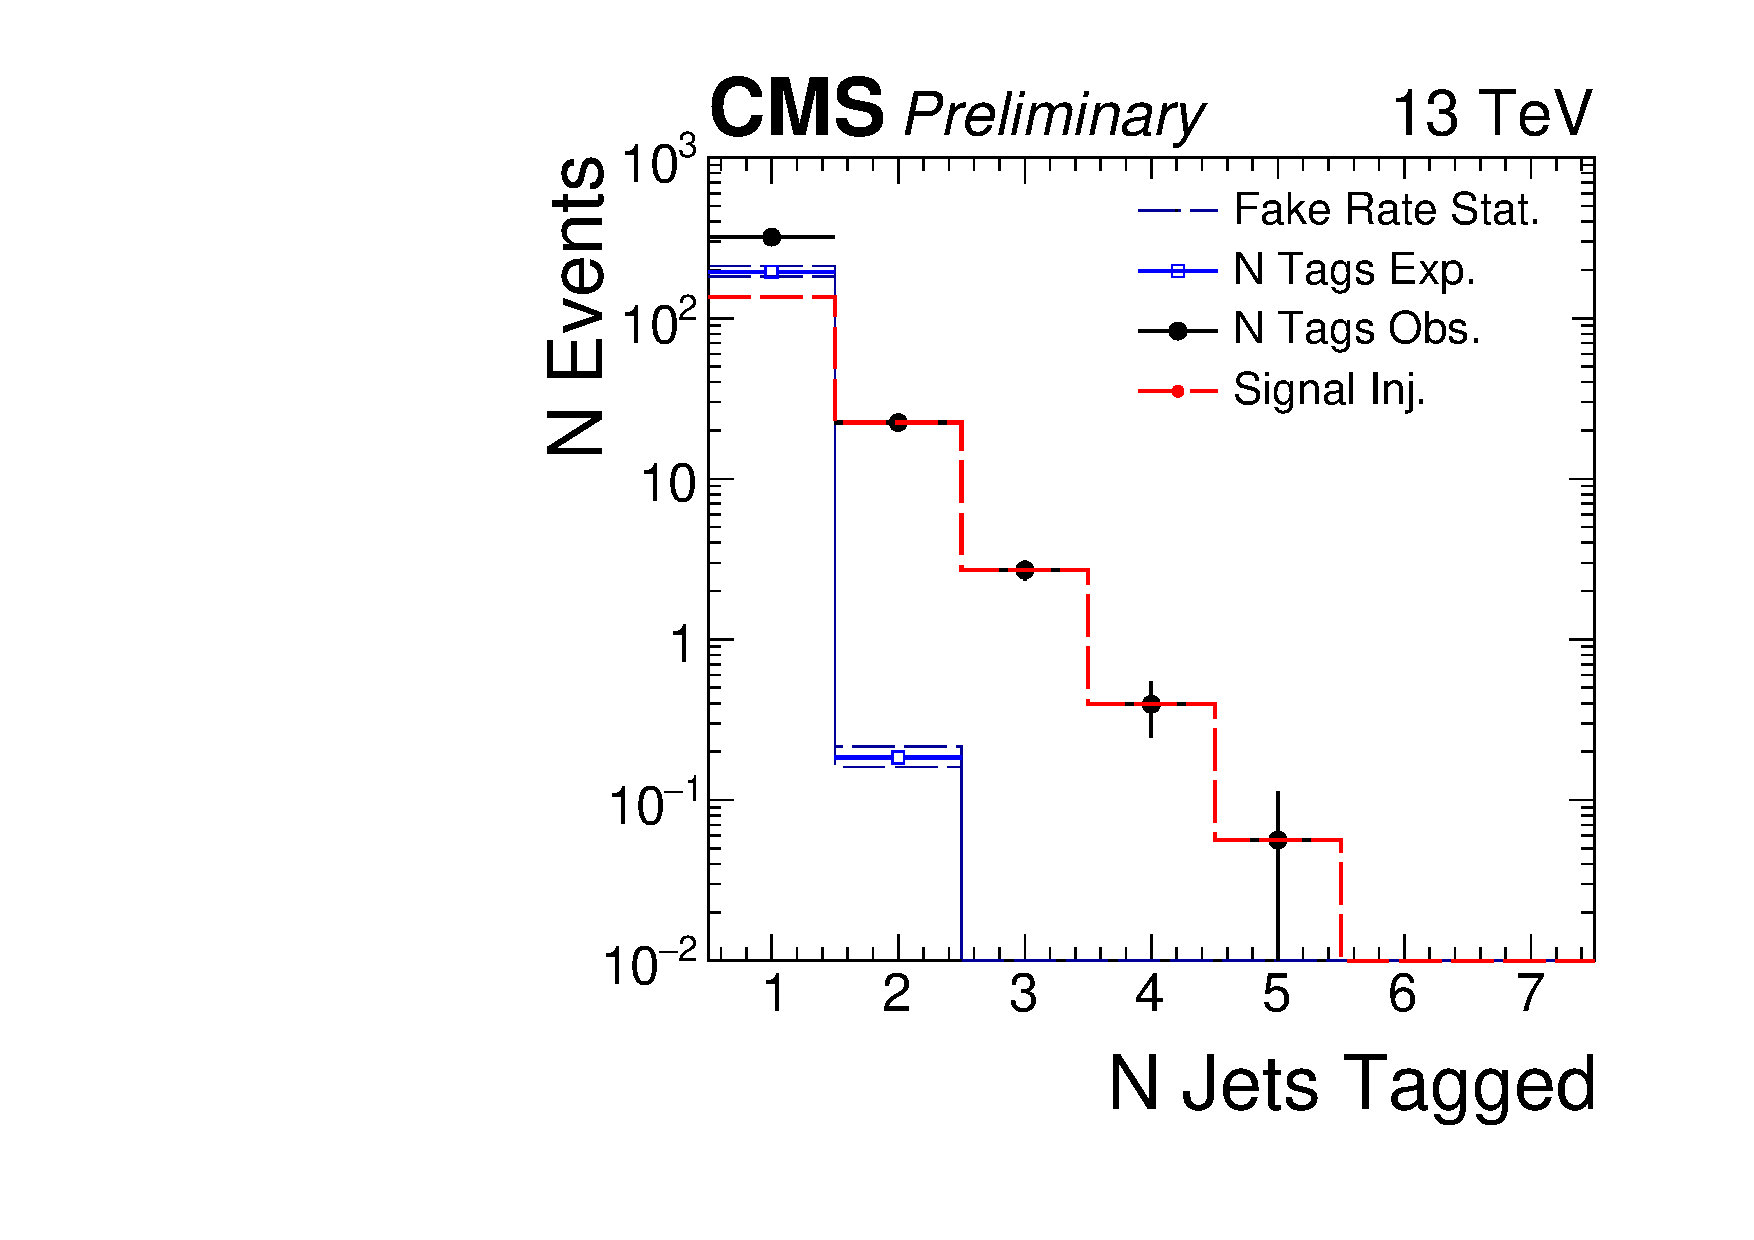
\includegraphics[width=.45\textwidth]{figures/an/ANALYSIS/76x_pu/INJECTION/mx100_ctau1000mm_1000ev.pdf}\\
\caption{Signal Injection. The Jet-Jet signal sample is varied $m_X=700$~GeV and $c\tau_0=1000$~mm (top left) 
$m_X=700$GeV and $c\tau_0=10$~mm (top right) $m_X=100$GeV and $c\tau_0=1000$~mm (bottom left) $m_X=100$~GeV and $c\tau_0=10$~mm (bottom right).
The level of signal contamination is fixed at 100 events for the $m_X=700$~GeV and 1000 events for $m_X=100$~GeV. The full 
event selection is applied and the baseline jet tag definition.  
\label{fig:injection_100gev_700gev_100ev}}
\end{center}
\end{figure}

\begin{table}
\caption{The signal injection test using a fixed signal point $m_{X} = 700$ ~GeV and $c\tau_0 = 10mm$ with varied amount of injection.
 A summary of the 1,2,3, and 4 tag predictions as a function of the number of events injected (top).  The two background systematic errors are
listed separately as $\sigma_{method},\sigma_{fake-rate}$. A summary of the observed number of tags (bottom). 
  \label{tab:700_injection_summary}}
\begin{center}
\begin{tabular}{cccccc}
\hline 
\textbf{Injection} $\sigma\times\mathcal{L}$  & \textbf{1 Pred} & \textbf{2 Pred} & \textbf{3 Pred} &\textbf{4 Pred} \\
\hline
0 &$ 185^{+14,+17}_{-14,-13} $&$0.16^{+0.01,+0.03}_{-0.01,-0.02}$& -- &-- \\
10 &$ 187^{+14,+17}_{-14,-13} $&$0.16^{+0.01,+0.03}_{-0.01,-0.02}$& -- &-- \\
100 &$ 207^{+16,+18}_{-16,-14} $&$0.20^{+0.02,+0.04}_{-0.02,-0.03} $&--&-- \\
1000 &$ 408^{+31,+23}_{-31,-19} $&$0.81^{+0.06,+0.09}_{-0.06,-0.08} $&--&-- \\
10000 &$ 2366^{+177,+53}_{-177,-49} $&$26.95^{+2.02,+1.19}_{-2.02,-1.10} $&$0.18^{+0.01,+0.01}_{-0.01,-0.01} $&-- \\
\hline 
\hline
\textbf{Injection} $\sigma\times\mathcal{L}$ & \textbf{1 Obs} & \textbf{2 Obs} & \textbf{3 Obs} & \textbf{4 Obs}\\
\hline
0 & 185.00 & 0.00 & 0.00 & 0.00 \\
10 & 186.94 & 2.40 & 1.99 & 1.20 \\ 
100 & 205.14 & 23.05 & 20.45 & 11.89 \\
1000 & 386.10 & 237.20 & 188.40 & 116.80 \\
10000 & 2260.00 & 2341.00 & 1976.00 & 1165.00 \\
\hline 
\end{tabular} 
\end{center}
\end{table}

\begin{table}
\caption{Signal injection test with fixed number of injected events and varied $c\tau_0$ and $m_X$. 
A summary of the 1,2,3, and 4 tag predictions as a function of the number of events injected (top). The two background systematic errors are
listed separately as $\sigma_{method},\sigma_{fake-rate}$.  A summary of the observed number of tags (bottom). 
\label{tab:700_100_injection_summary}}
\begin{center}
\begin{tabular}{cccccc}
\hline 
$\sigma\times\mathcal{L}$ & $m_X$ [GeV] & $c\tau_0$ [mm]  & \textbf{1 Pred} & \textbf{2 Pred} & \textbf{3+4 Pred} \\
\hline
100 &$ 700 $&$ 10 $&$ 207^{+16,+18}_{-16,-14} $&$0.20^{+0.02,+0.04}_{-0.02,-0.03} $&-- \\
100 &$ 700 $&$ 1000 $&$ 202^{+15,+18}_{-15,-14} $&$0.20^{+0.02,+0.03}_{-0.02,-0.03} $&--\\
1000 &$ 100 $&$ 10 $&$222^{+17,+18}_{-17,-14} $&$0.23^{+0.02,+0.04}_{-0.02,-0.03} $&--\\
1000 &$ 100 $&$ 1000 $&$ 195^{+15,+17}_{-15,-13} $&$0.18^{+0.01,+0.03}_{-0.01,-0.02} $&--\\ 
\hline 
\hline 
$\sigma\times\mathcal{L}$ & \textbf{Mass} [GeV] & $c\tau_0$ [mm]  & \textbf{1 Obs} & \textbf{2 Obs} & \textbf{3+4 Obs}  \\
\hline
100 & 700 & 10 & 205.14 & 23.05 & 32.34 \\
100 & 700 & 1000 & 211.56 & 17.98 & 12.36  \\
1000 & 100 & 10 & 403.57 & 74.33 & 26.10 \\
1000 & 100 & 1000 & 320.64 & 22.92 & 3.99  \\
\end{tabular} 
\end{center}
\end{table}

\begin{table}[tb]
  \caption{A summary of the size of the signal injected in the signal injection test (top).
    A summary of signal region yields in the 2,3, and 4 nominal displaced jet tag bins (middle) and  the
    observed number of tags (bottom), as a function of the
    size of the signal contamination, for a signal injection test using a fixed
    signal point $m_{X} = 700$ ~GeV and $c\tau_0 = 10$~mm with
    varied signal yields. The no signal case is included as a reference to 
    the predicted values without contamination. The test is normalized such that the sum of signal and background
     events stays fixed at the observed number of events passing the analysis event selection.
    The contamination fraction corresponds to the hypothetical fraction of signal events contained within
     the events passing the event selection.  
    \label{tab:700_injection_summary_norm}}
\begin{center}
\begin{tabular}{cccc}
\textbf{Contam. Fraction} & \textbf{Signal} $\sigma$ [fb] \\ 
\hline
 0 & 0 \\
 0.01\% & 30 \\
 0.10\% & 290 \\
 1.04\% & 3000 \\
 9.47\% & 28000 \\
\end{tabular} 
\begin{tabular}{ccccc}
\textbf{Contamination \%} & \textbf{2 tag pred} & \textbf{3 tag pred} &\textbf{4 tag pred} \\
\hline
 0 &  $1.34^{+0.25}_{-0.17}$ & - & - \\ 
 0.01\% & $1.34^{+0.25}_{-0.17}$ & - & - \\
 0.10\% & $1.67\pm0.33$ & - & - \\
 1.04\% & $6.71^{+0.91}_{-0.82}$ &- & - \\
 9.47\% & $205.38\pm15.21$ & $1.37\pm0.08$ & - \\ 
\\
\textbf{Contamination \%} &  \textbf{2 tag obs} & \textbf{3 tag obs} & \textbf{4 tag obs} \\
\hline
0.00\% & 0 & 0 & 0 \\
0.01\% &  19 & 16 & 10 \\ 
0.10\% &  179 & 159 & 93 \\
1.04\% &  1914 & 1520 & 943   \\
9.47\% &  17632  & 14883 & 8775   \\
\end{tabular} 
\end{center}
\end{table}

To test the response of the background prediction to the presence of signal contamination in the jet probabilities used for the $P(N_{tags})$ derivation,
signal events are `injected` into QCD Monte Carlo. Approximately 15 million QCD events from /QCD\_HT700to1000\_TuneCUETP8M1\_13TeV-madgraphMLM-pythia8 are used as the background input.
The resulting predictions for varied masses, lifetimes, and sizes of contamination are shown in Fig. \ref{fig:injection_700_10mm} and Fig. \ref{fig:injection_100gev_700gev_100ev}. The corresponding predictions, observed number of tags, and the
deviation from expectation are summarized in Table \ref{tab:700_injection_summary}  and Table \ref{tab:700_100_injection_summary}. The goal of this exercise
is to understand the quantity of signal contamination, as well as lifetime and mass, required to significantly alter the background prediction. 

The resulting predictions are also reported normalized such that the total signal + qcd events passing the event selection are equal to the number of events passing the
event selection in the analysis in Table \ref{tab:700_injection_summary_norm}.

The change in the $N_{tags}^{obs}$ distribution to the presence of signal is on the order of the number of events with $N_{tags}>2$ whereas 
the integrated shift in $P(N_{tags}\geq2)$ is on the order of the shift induced in the $p(j)$ distribution. This shift is of the order the signal contamination. 
We can conclude the analysis will retain relative sensitivity as long as the signal contamination is relatively smaller than the QCD contribution in 
the fake rate calculation. 

In summary, the background prediction is robust to a variety signal masses, lifetimes and sizes of contamination. Robust in the sense that the
background is correctly determined within error in the 0 injection case and the bias to the background prediction due to the 
contamination is small relative to the number of signal events injected.

The following section explores the  sensitivity to signal explicitly in a simplified scenario given the assumption that the jet probabilities accurately predict the
background in the scenario where there are no signal events present. This assumption is based on on the the closure studies in the previous section and be considered
true within some closure systematic.

\subsubsection{Explicit Sensitivity in A Simplified Injection Scenario}

Consider a sample of $N_{QCD}$ QCD events with a known fraction of jets that are tagged $f(j_i)$ as a function of some jet parameters $j_i$. 
For simplicity, assume events have exactly 2 jets. Also assume 
we have shown that the observation approximately determined $N_{obs}^{2tag} = N_{pred}^{2tag}$ when we interpret $f(j_i)$ as a conditional probability 
$p(j_i)$ such that:
\begin{align*}
N_{obs}^{2tag} = N_{pred}^{2tag} = \sum_i [p(j_1)p(j_2)]_{i}  = N_{QCD}p^2 
\end{align*}
where we are using a flat probability $p$ such that  $p(j_1)=p(j_2)=p=n_{tag}/n_{jets} =  n_{fake} / 2N_{events}$. Where $n_{tag}$ is the number of jets tagged, which 
in a QCD sample is exactly $n_{fake}$. Now, say we perform the signal injection test by
injecting $N_{sig}$ events with correspondingly $2N_{sig}$ signal jets. Let $\epsilon$ be the efficiency for a signal event to have 1 tag. 
 Accordingly the probability will shift $p(j_i)\rightarrow \tilde{p}(j_i)$:
\begin{align*}
\tilde{p} = \frac{n_{fake} + n_{true-tags}}{2N_{QCD} + 2N_{sig}} = \frac{n_{fake} + \epsilon 2N_{sig} }{2N_{QCD} + 2N_{sig}}
\end{align*}
Taylor expanding in $N_{sig}$ about 0 we obtain:
\begin{align*}
\tilde{p} &= \frac{n_{fake}}{2N_{QCD}} - \frac{N_{sig}n_{fake}}{2(N_{QCD})^2} + \epsilon\frac{2N_{sig} N_{QCD}}{2(N_{QCD})^2}\\
&= p - p\frac{N_{sig}}{N_{QCD}} + \frac{N_{sig}\epsilon}{N_{QCD}}
\end{align*}
Let $\Delta = N_{sig}/{N_{QCD}}$
\begin{align*}
\tilde{p} = p(1-\Delta) + \Delta\epsilon
\end{align*}
Note that as the signal contamination  $\Delta\rightarrow 0$, we obtain the correct probability $\tilde{p}=p$. 
Now we attempt to predict the number of events with 2 tags using $\tilde{p}$ and splitting the sum over signal and QCD events.
\begin{align*}
N_{pred}^{2tag} &= \sum_i \tilde{p}\tilde{p}\\ 
&= \sum_i (p(1-\Delta) + \Delta\epsilon)^2\\ 
&= \sum_i p^2 - p^2(2\Delta) + p^2\Delta^2 + 2p\Delta \epsilon - 2 p \Delta^2 \epsilon + \Delta^2 \epsilon^2
\end{align*}
We now split the events in the sum between QCD and Signal. 
\begin{align*}
N_{pred}^{2tag} &= \sum_i (QCD) + \sum_i (Signal)\\
\sum_i (QCD) &= N_{QCD} ( p^2 - p^2(2\Delta) + p^2\Delta^2 + 2p\Delta \epsilon - 2 p \Delta^2 \epsilon + \Delta^2 \epsilon^2)\\
&= N_{obs}^{QCD} - N_{sig}(p^2\Delta + \Delta \epsilon^2 - 2p^2 + 2p\epsilon - 2p\Delta \epsilon) 
\end{align*}
where we have used the fact that $\Delta N_{QCD} = N_{sig}$ and $\sum_i p^2 = N_{obs}^{QCD}$:
\begin{align*}
\sum_i(Signal) =  N_{sig}(  p^2 - p^2(2\Delta) + p^2\Delta^2 + 2p\Delta \epsilon - 2 p \Delta^2 \epsilon + \Delta^2 \epsilon^2)
\end{align*}
We now evaluate our sensitivity to signal or equivalently the disagreement between observed and prediction by the variable $S$. Let 
$N_{obs}^{2tag} = N_{obs}^{sig} + N_{obs}^{QCD}$. The sensitivity $S$, is a measure of how well we have predicted the background
in the presence of signal. When $S=1$ the prediction is exactly the background and the excess is exactly the number of signal events. 
When $S=0$ the probabilities prediction has over estimated the background entirely resulting in no disagreement between observed and predicted 
2 tag events.
\begin{align*}
S = \frac{N_{obs}^{2tag} - N_{pred}^{2tag} }{N_{sig}} = 1 &- (2p\epsilon + \Delta \epsilon^2) \\
&- (p^2 + \Delta^2\epsilon^2 +  2p\Delta\epsilon -2p^2  - 2p\Delta\epsilon) \\
&- (p^2\Delta -2p^2\Delta -2p\Delta^2\epsilon) \\
&- (p^2\Delta^2)
\end{align*}
where we have grouped terms by their order in $O(\Delta)+O(p)$. Consider the case when
$\epsilon \approx 1$ (this is an approximation for readability as $\epsilon=1$ would imply no 2 tag events) and for simplicity say $\Delta = p = x$.
\begin{align*}
S= 1 - 3x + 3 x^3 - x^4
\end{align*}
If we plug in the baseline fake rate for $x$  then $S(x=5\times10^{-4})= 0.999$. 

\subsection{Tag Probability Cross Validation}
\label{sec:xval}

To test the bias of the background estimation a method of cross validation is utilized. For a given sample, $N_{div}$ non-overlapping  sub-samples are partitioned. 
For each sub-sample, a corresponding set of jet probabilities are computed as described in the previous section. 
For each set of jet probabilities, an $N_{tag}^{pred}$  prediction is made for the $N_{div}-1$ remaining samples (which have no overlapping events). We will
refer to the sample use for the prediction as the measurement sample. The result is $N_{div}(N_{div}-1)$ pairs of probabilities and measurement samples. 
From each pair, in each bin of $N_{tags}$, we  generate a distribution of pulls $(N_{obs} - N_{pred}) / \sqrt{N_{pred}}$ for each $N_{tag}$ bin. All events must pass the event selection.

Due to limited statistics in the 2 tag bin for the baseline tag, the loose tag definition (Table \ref{tab:loose_tag_def}) is used to generate pull distributions in the 2 tag bin. 

\begin{figure}
\begin{center}
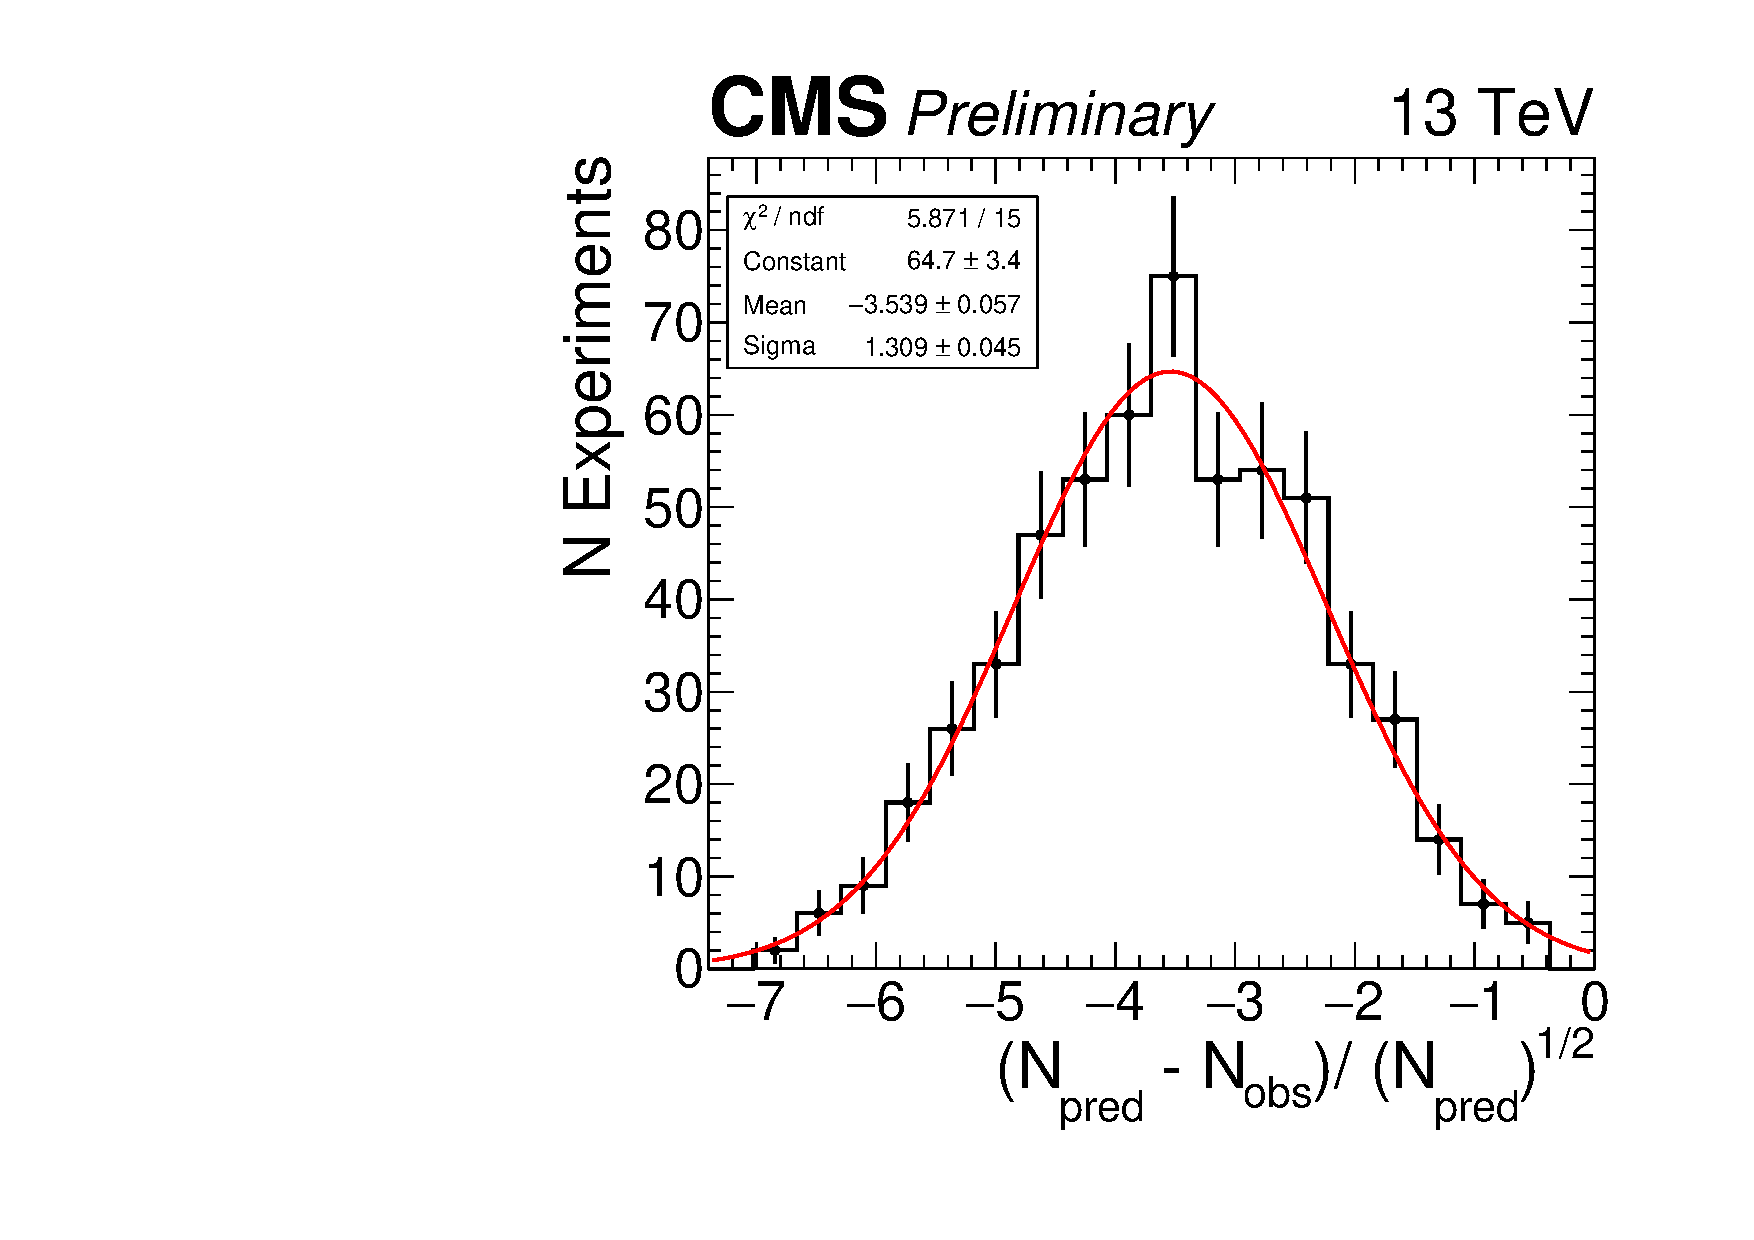
\includegraphics[width=.45\textwidth]{figures/an/ANALYSIS/pulls/data_loose_uncorrected_1tag.pdf}
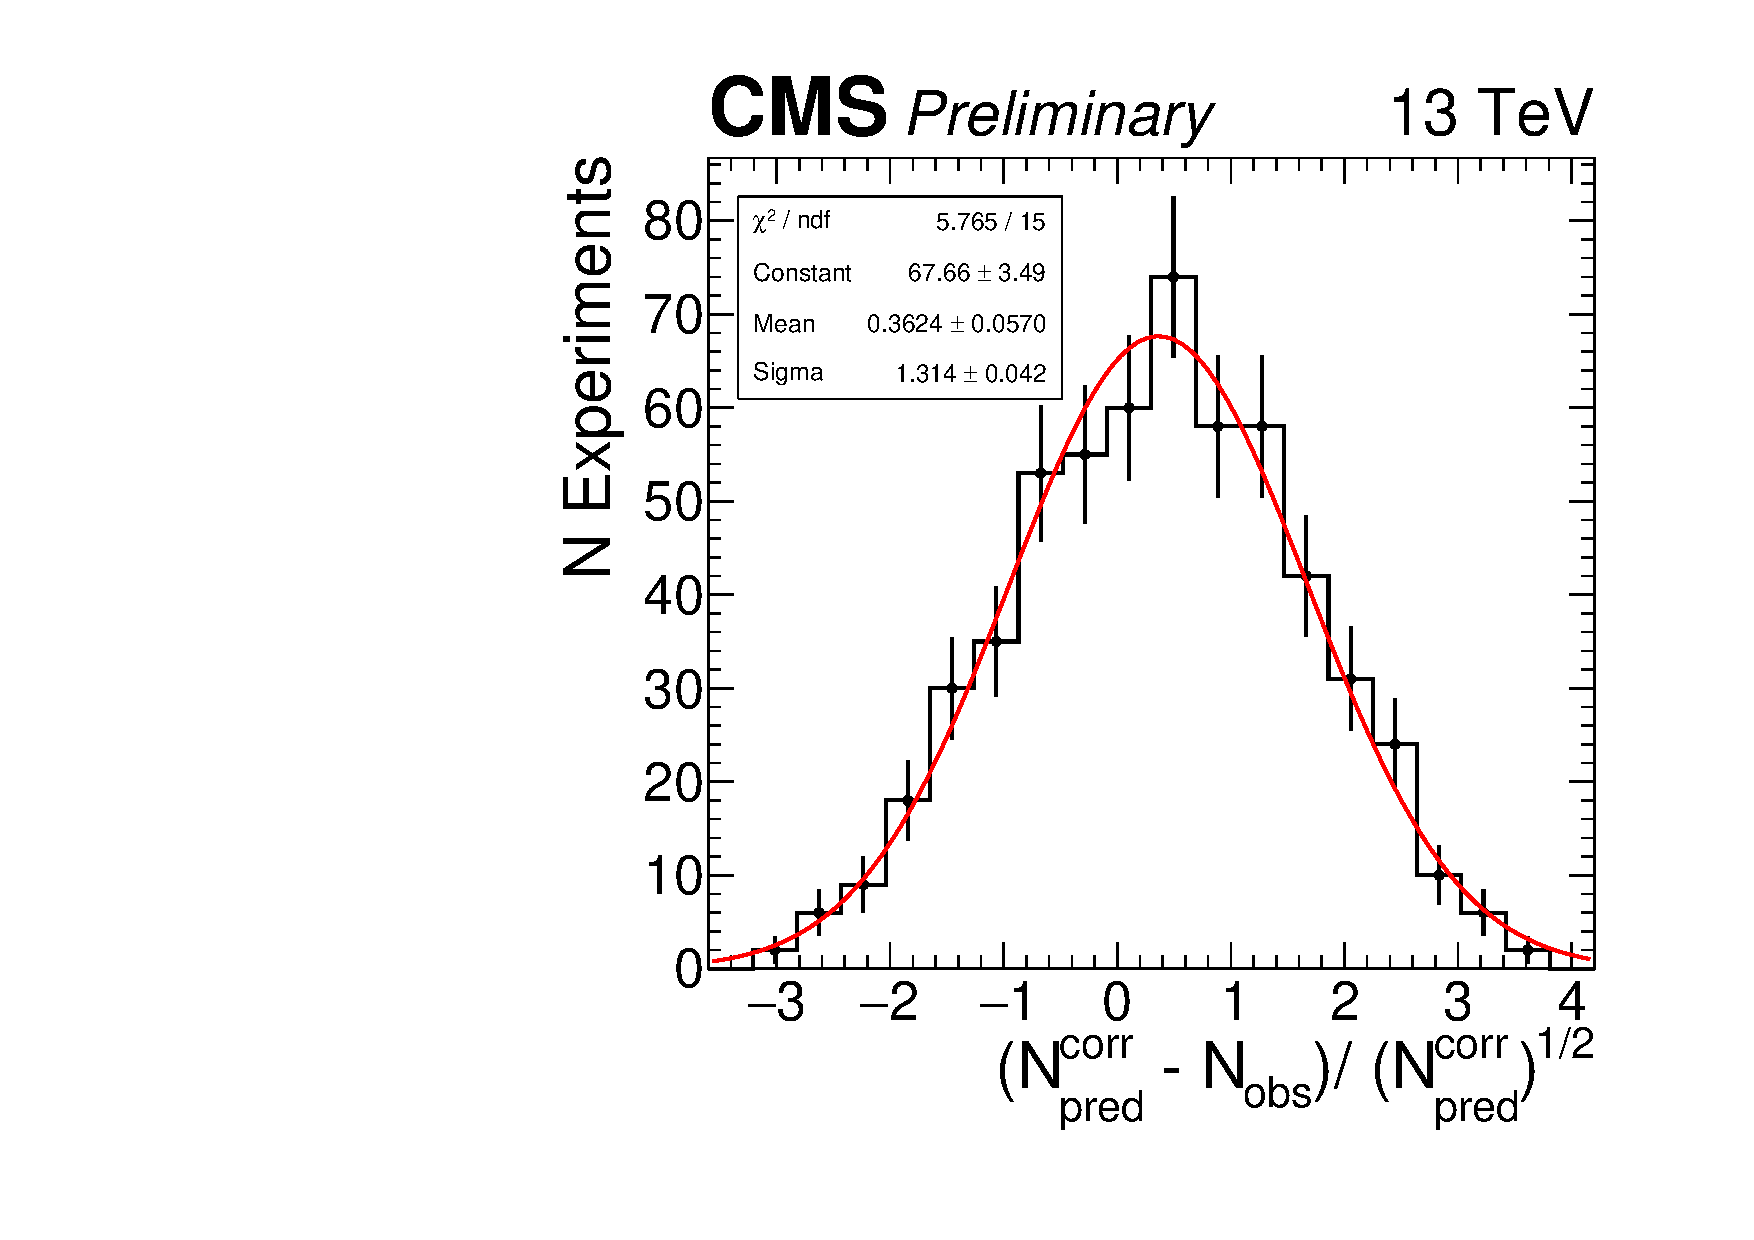
\includegraphics[width=.45\textwidth]{figures/an/ANALYSIS/pulls/data_loose_corrected_1tag.pdf}
\caption{Cross validation of the predicted of the number of loose tags in data collected by the displaced jet triggers. Pulls for the 1 tag bin with the loose tag (left). Pulls for the 1 tag bin with the loose tag with the SR correction (Right).   \label{fig:djetpd_1tag_xval}}
\end{center}
\end{figure}

\begin{figure}
\begin{center}
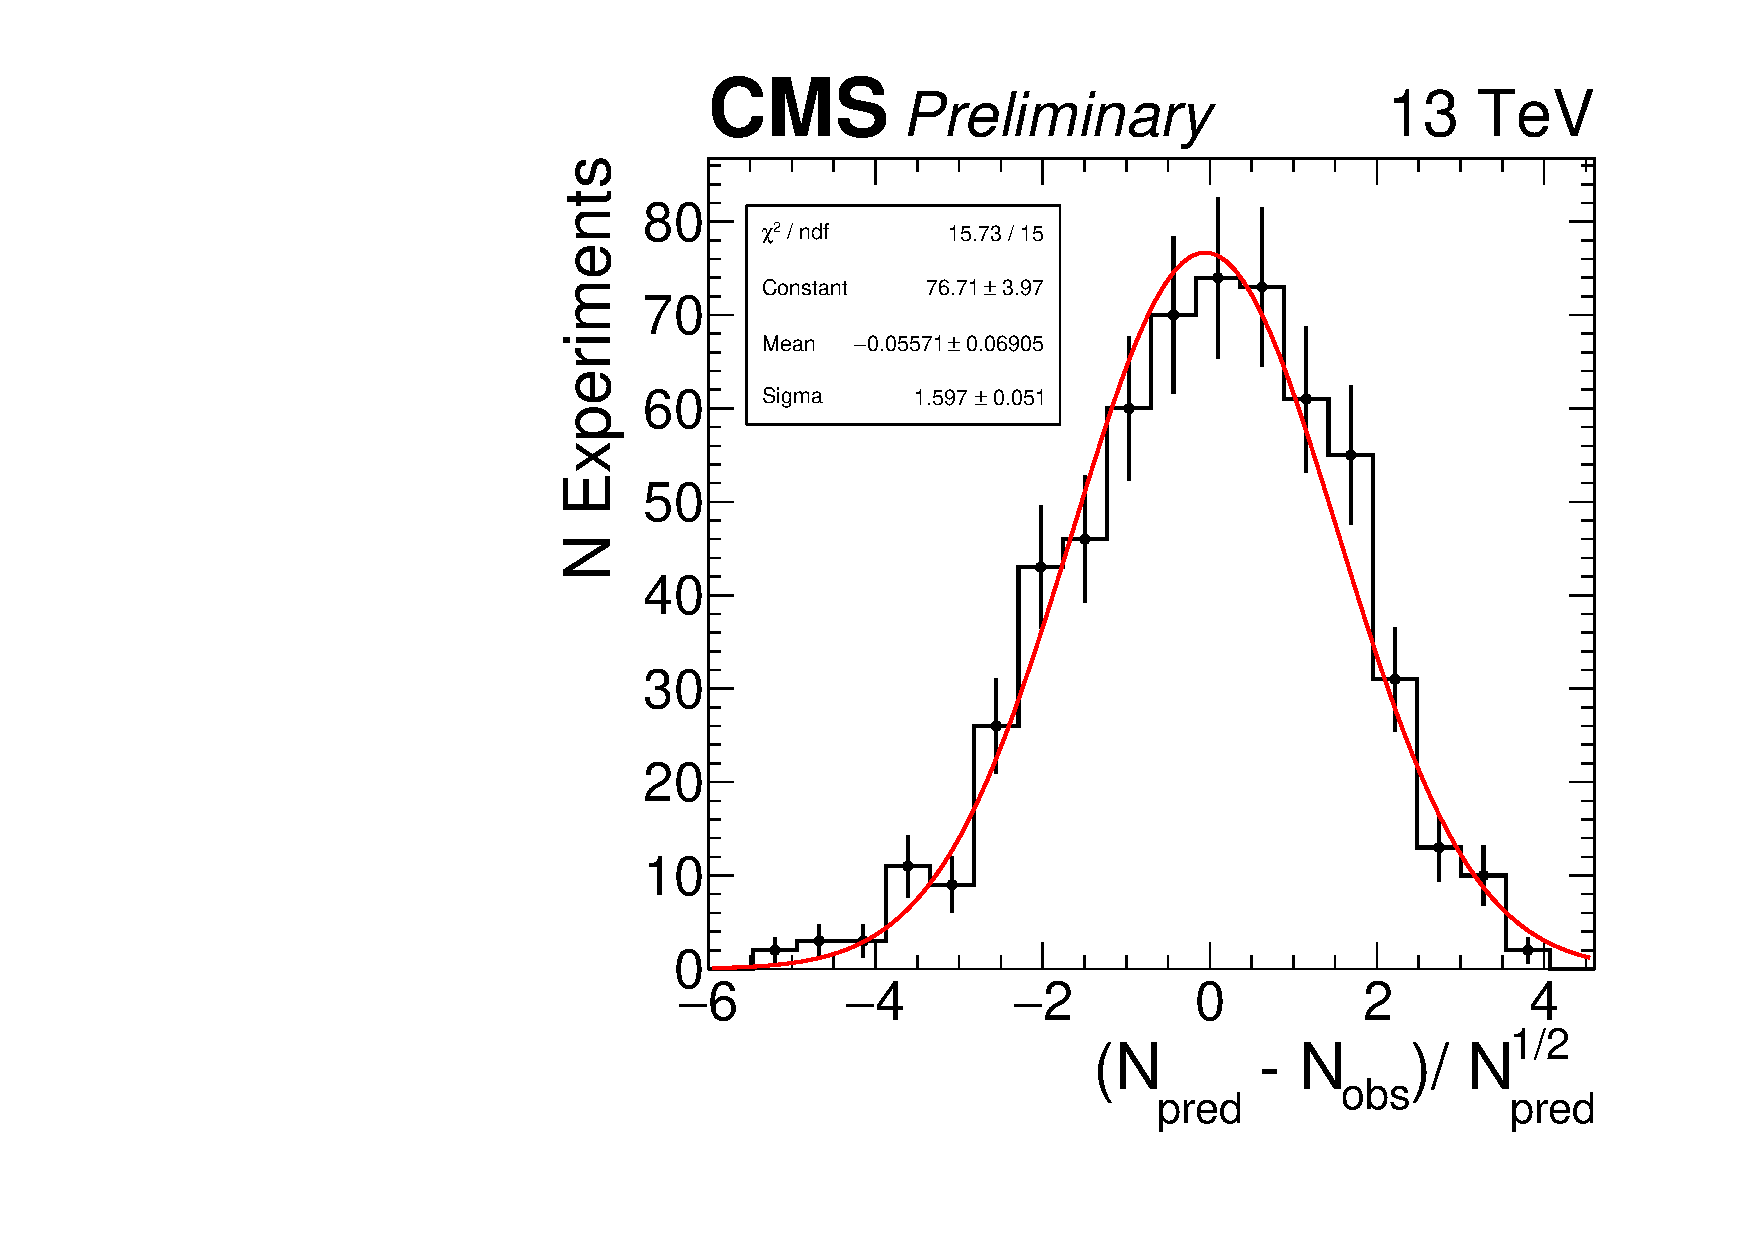
\includegraphics[width=.45\textwidth]{figures/an/ANALYSIS/pulls/baseline_xval_ndiv25_baseline_1tag.pdf}
\caption{Cross validation of the predicted of the number of tags in data passing the displaced jet triggers. Pulls for the 1 tag bin with the baseline tag after the application of the signal removal correction $2r_{12}=.2\%$ \label{fig:djetpd_1tag_xval_baseline}}
\end{center}
\end{figure}


\begin{figure}
\begin{center}
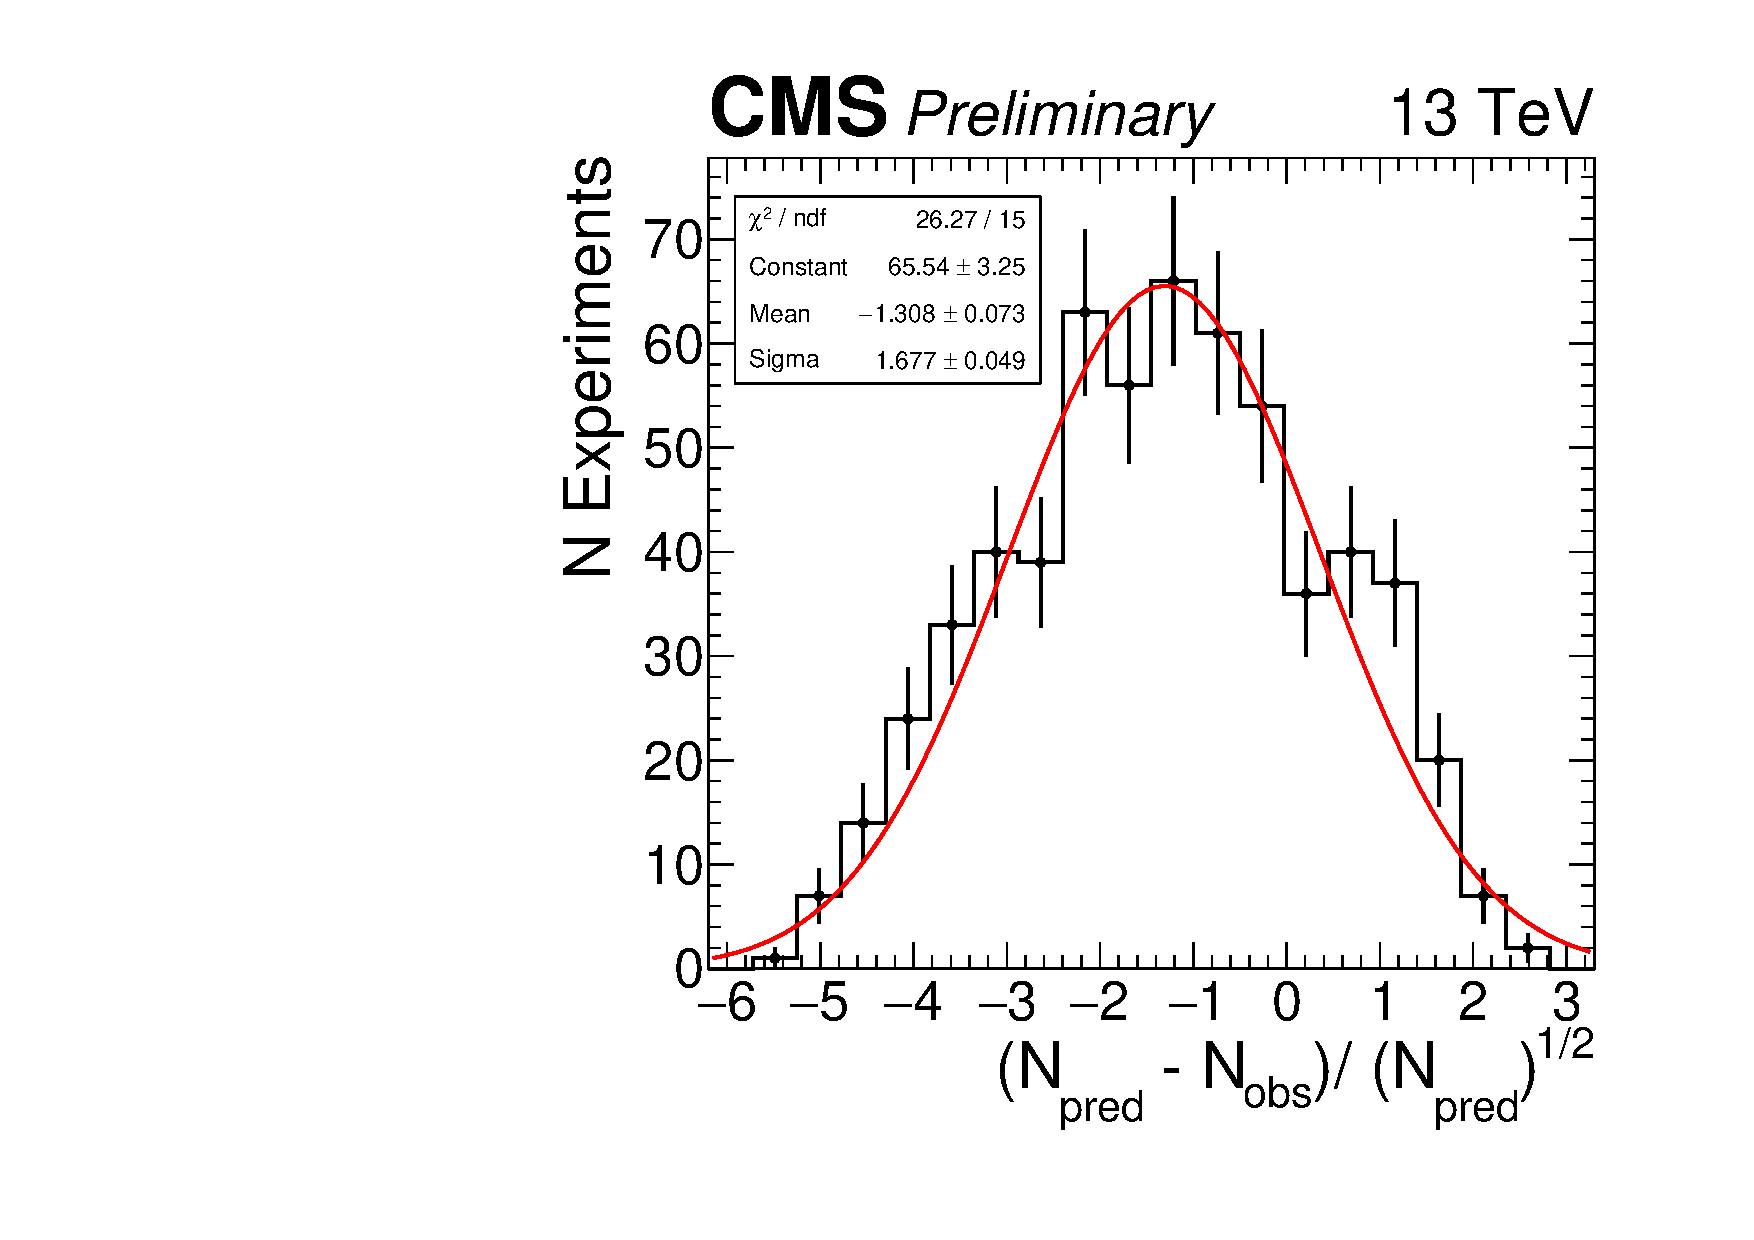
\includegraphics[width=.45\textwidth]{figures/an/ANALYSIS/pulls/qcd_loose_uncorrected_1tag.pdf}
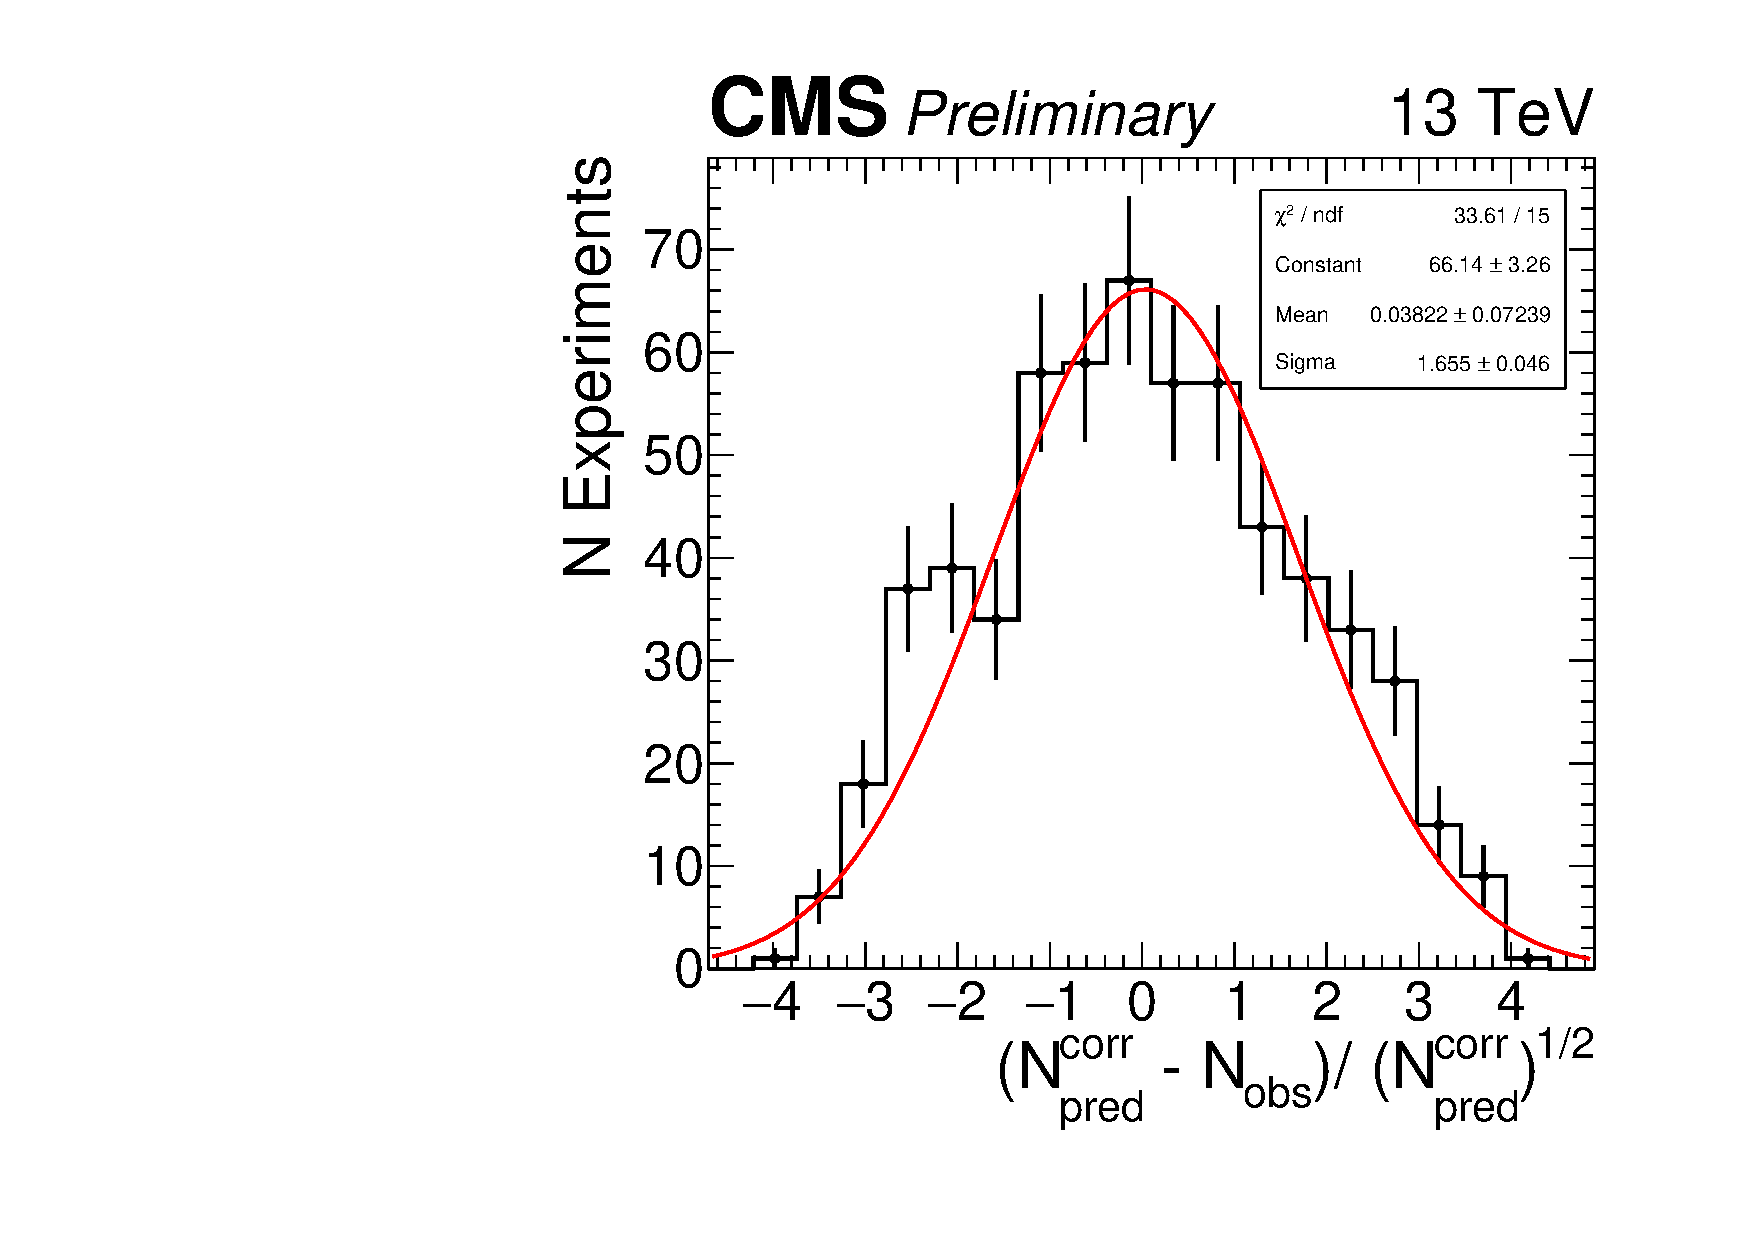
\includegraphics[width=.45\textwidth]{figures/an/ANALYSIS/pulls/qcd_loose_corrected_1tag.pdf}
\caption{Cross validation of the predicted of the number of loose tags in QCD events passing the displaced jet triggers. Pulls for the 1 tag bin with the loose tag (left). The signal region removal corrected pulls (Right). \label{fig:qcd_1tag_xval}}
\end{center}
\end{figure}

\begin{figure}
\begin{center}
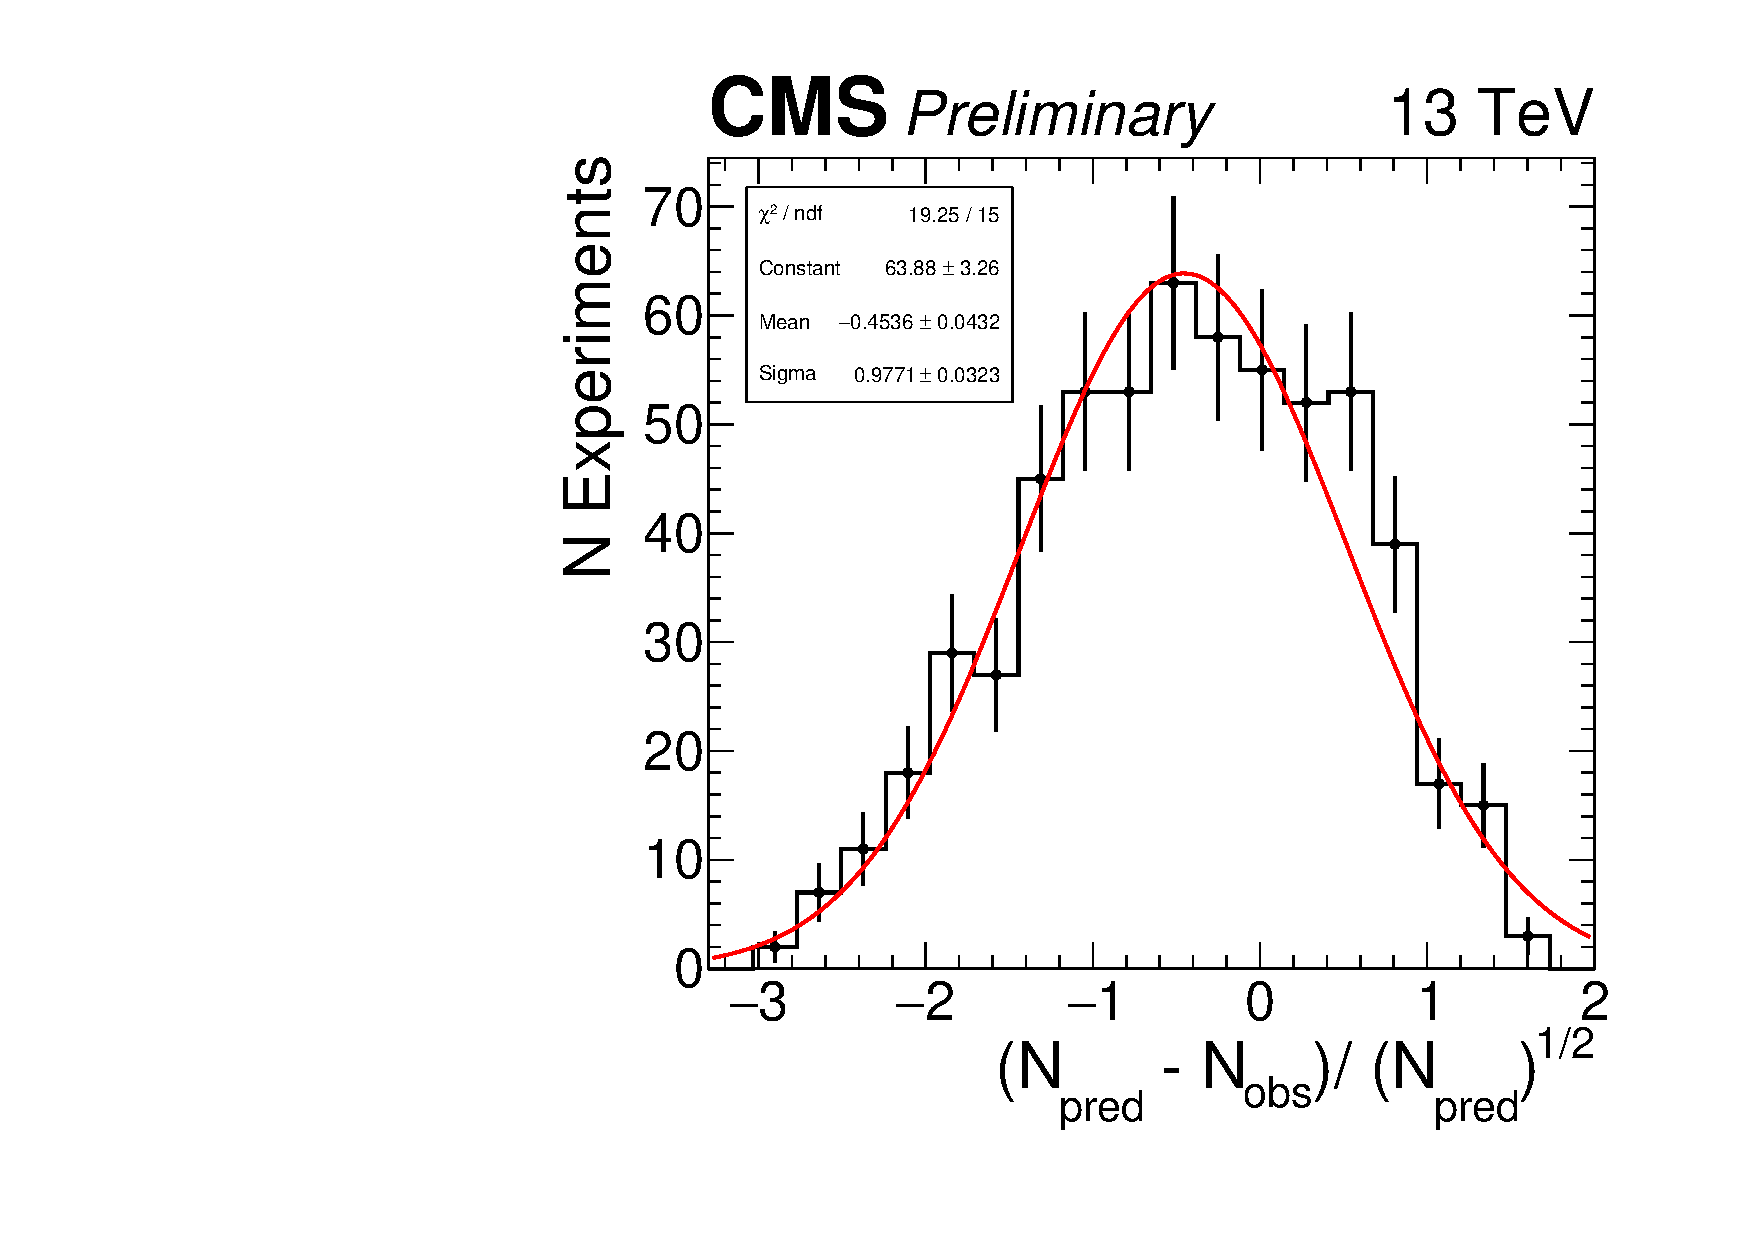
\includegraphics[width=.45\textwidth]{figures/an/ANALYSIS/pulls/qcd_loose_uncorrected_2tag.pdf}
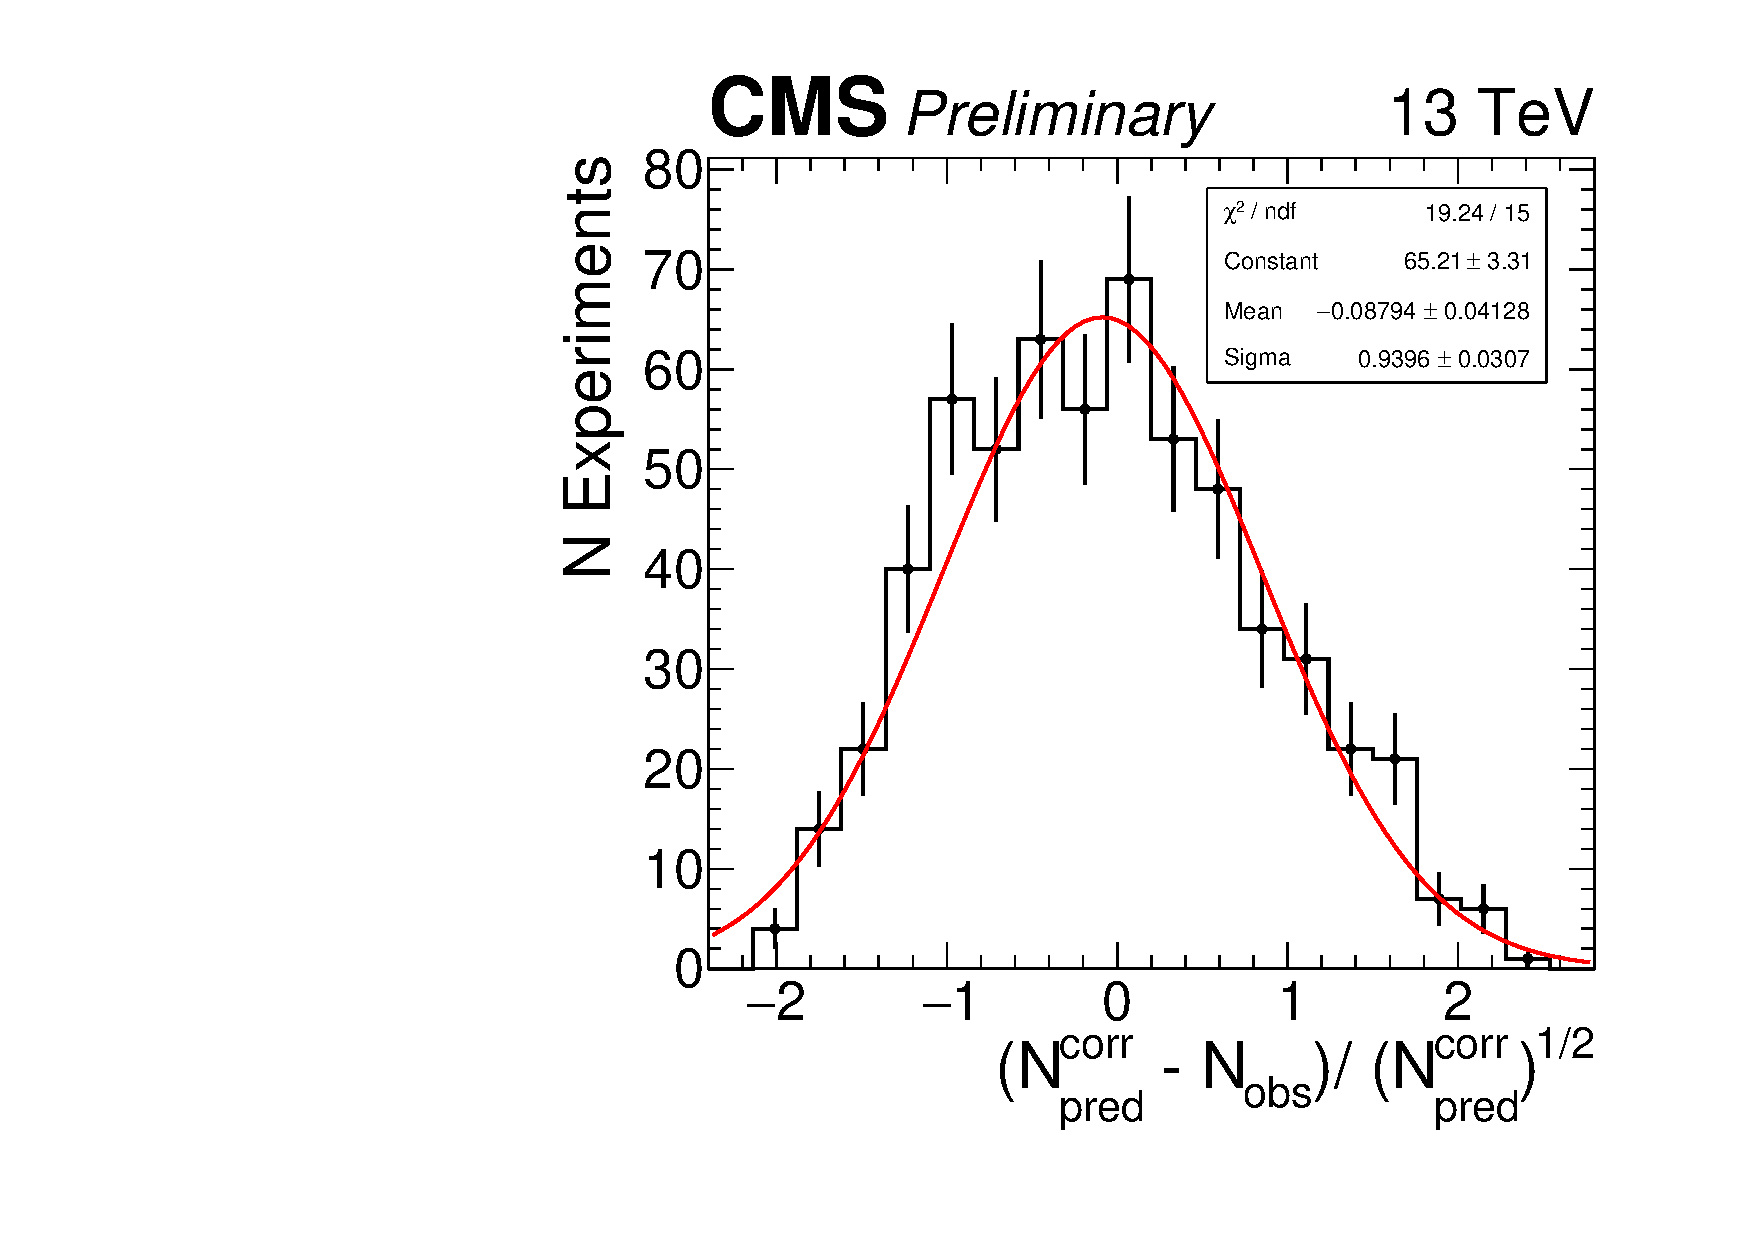
\includegraphics[width=.45\textwidth]{figures/an/ANALYSIS/pulls/qcd_loose_corrected_2tag.pdf}
\caption{Cross validation of the predicted of the number of loose tag in QCD events passing the displaced jet triggers. Pulls for the 2 tag bin with the loose tag uncorrected (left). The same prediction corrected for the SR removal (right) \label{fig:qcd_2tag_xval}}
\end{center}
\end{figure}


\begin{figure}
\begin{center}
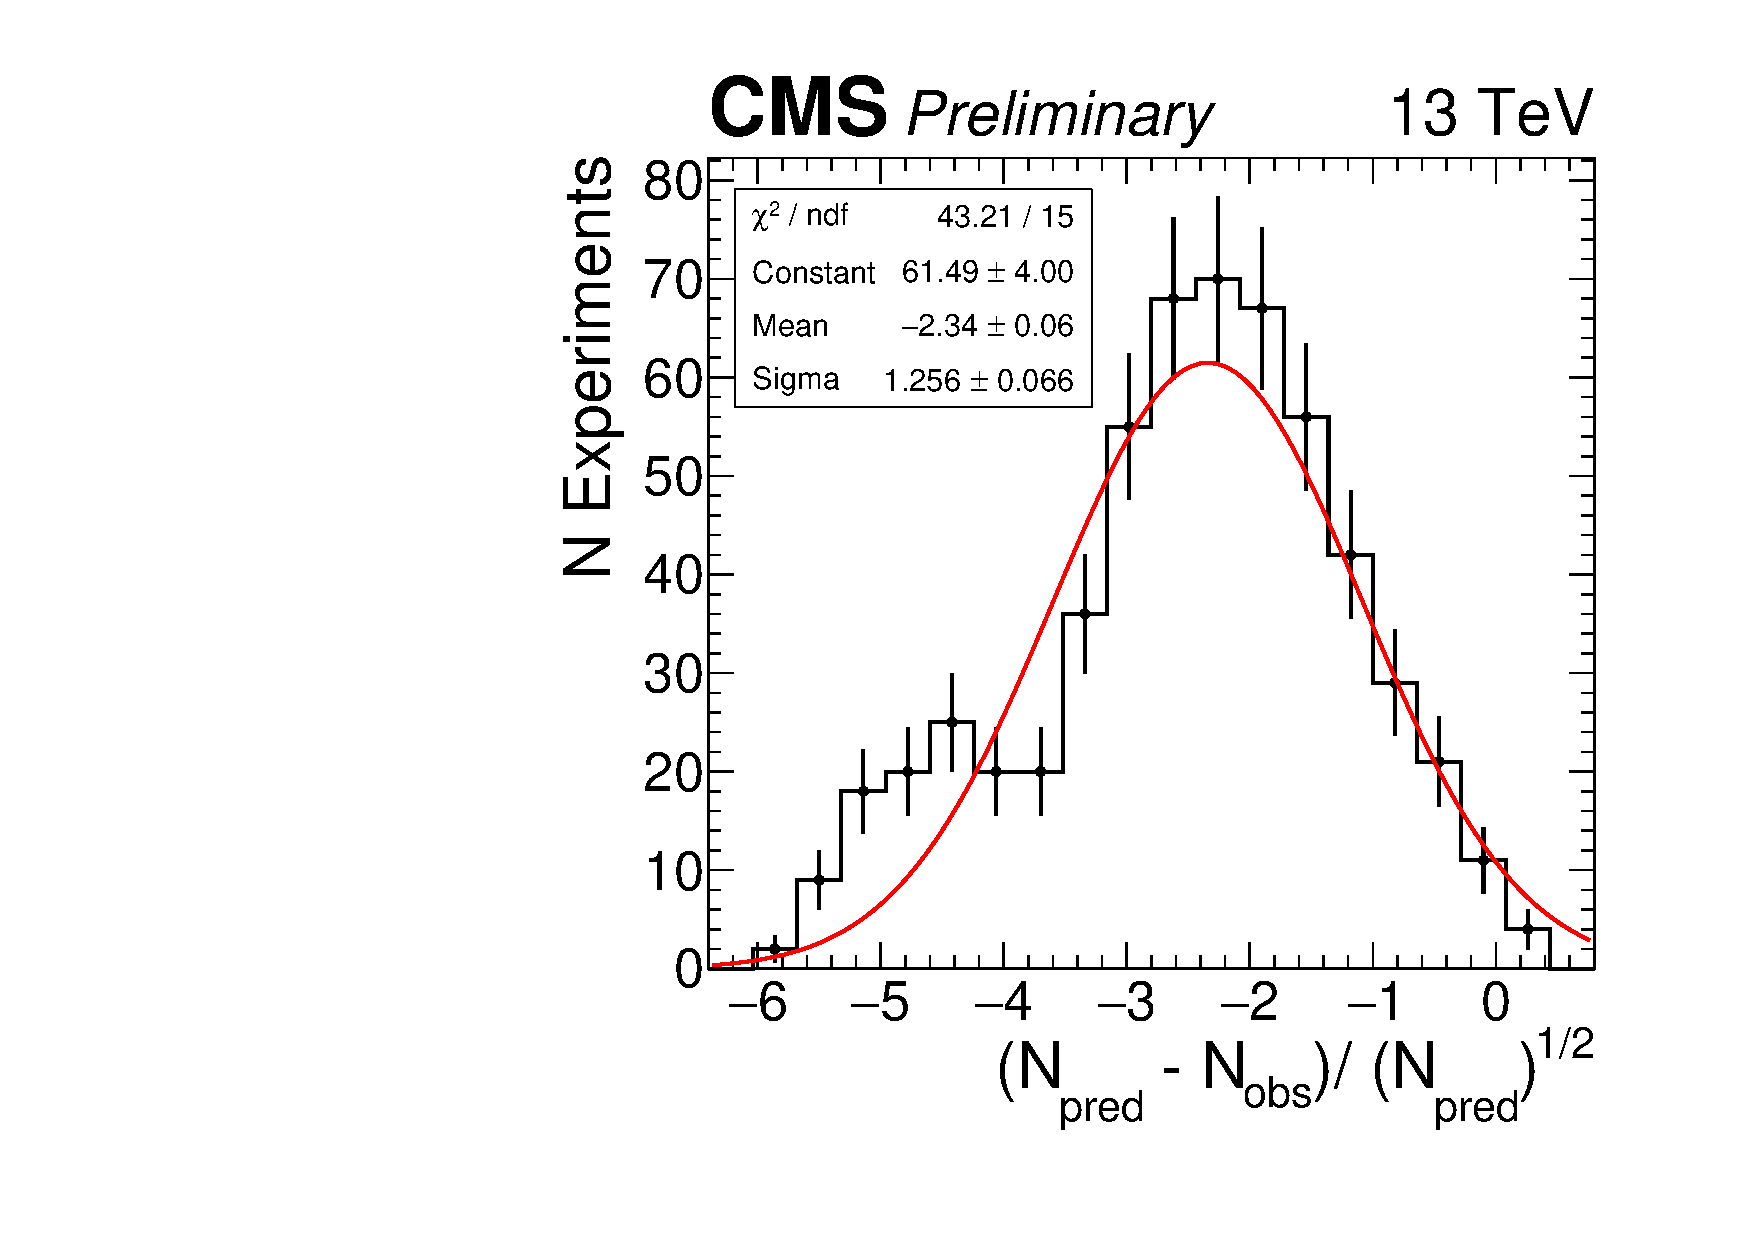
\includegraphics[width=.31\textwidth]{figures/an/ANALYSIS/pulls/data_loose_uncorrected_2tag.pdf}
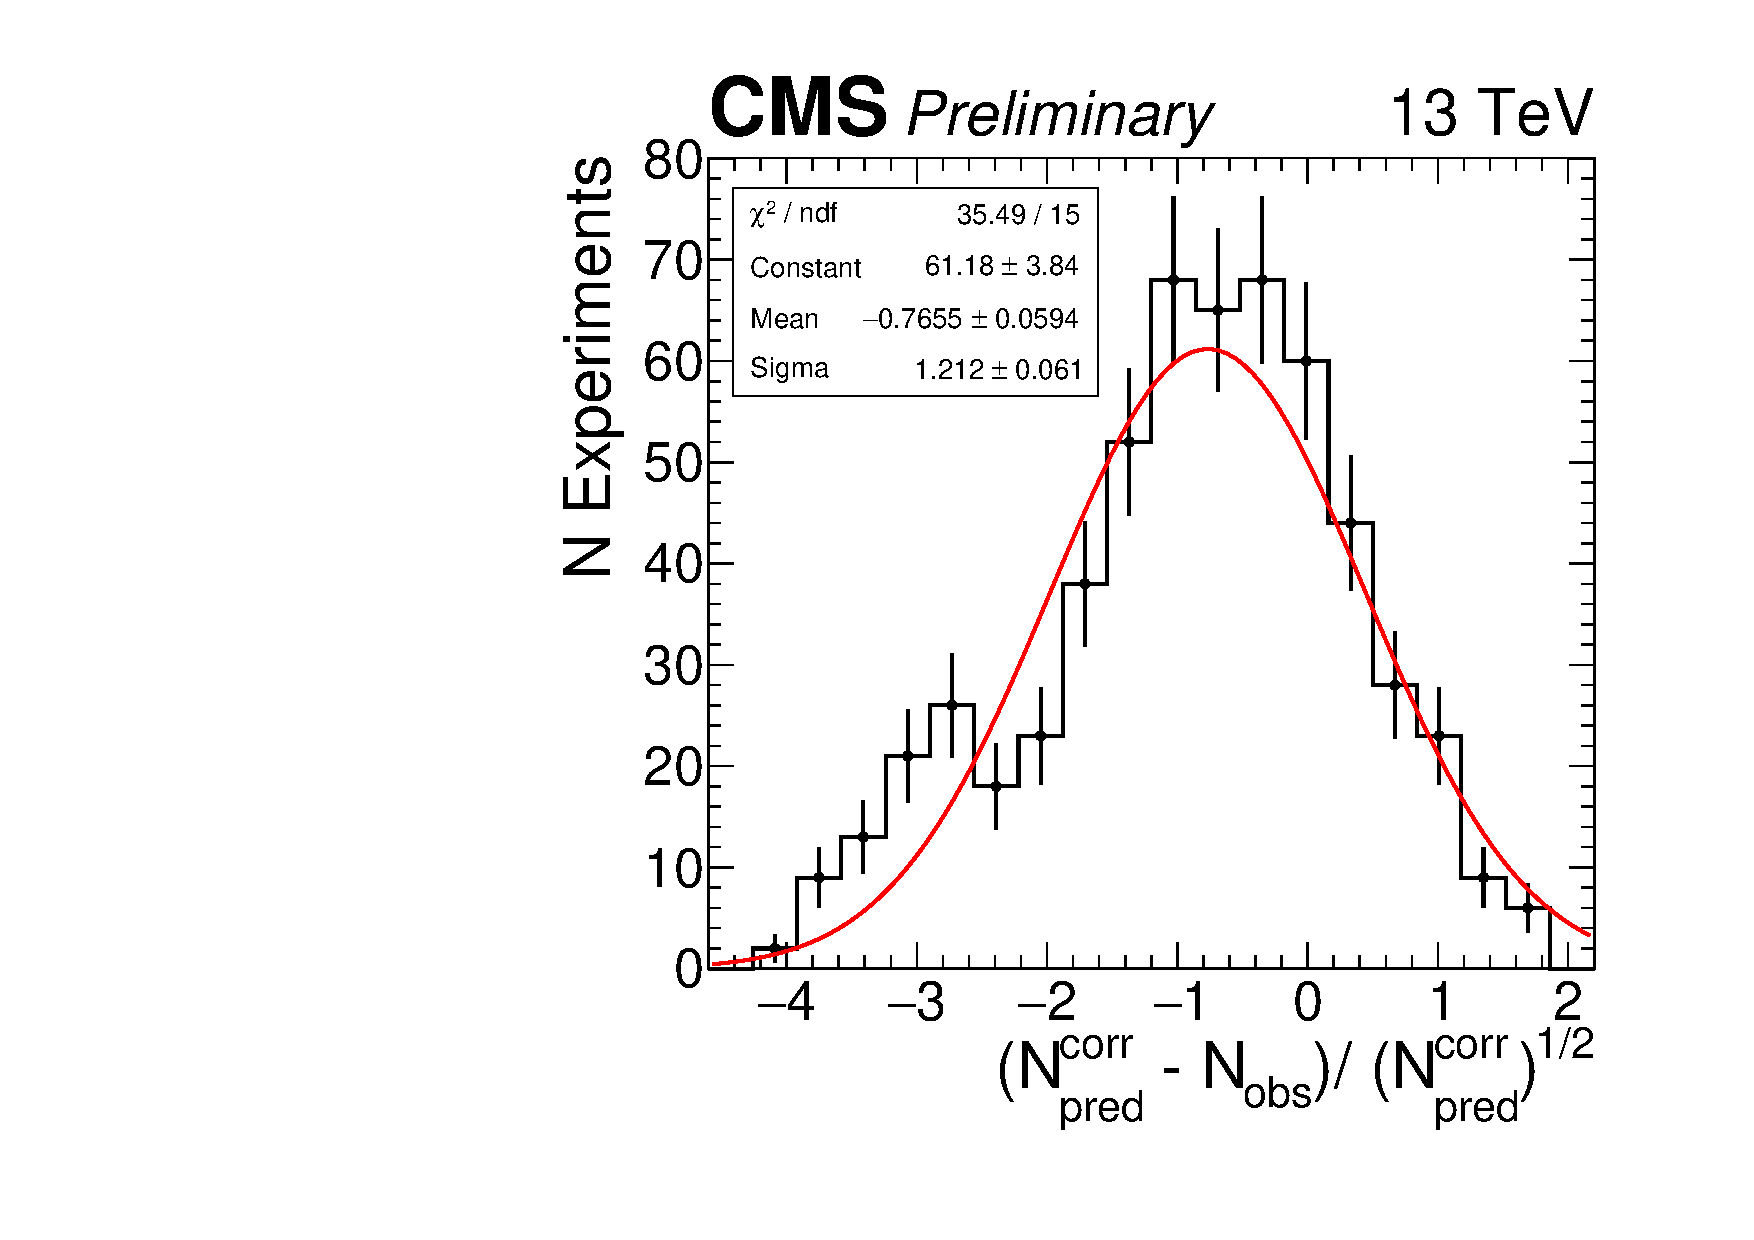
\includegraphics[width=.31\textwidth]{figures/an/ANALYSIS/pulls/data_loose_corrected_2tag.pdf}
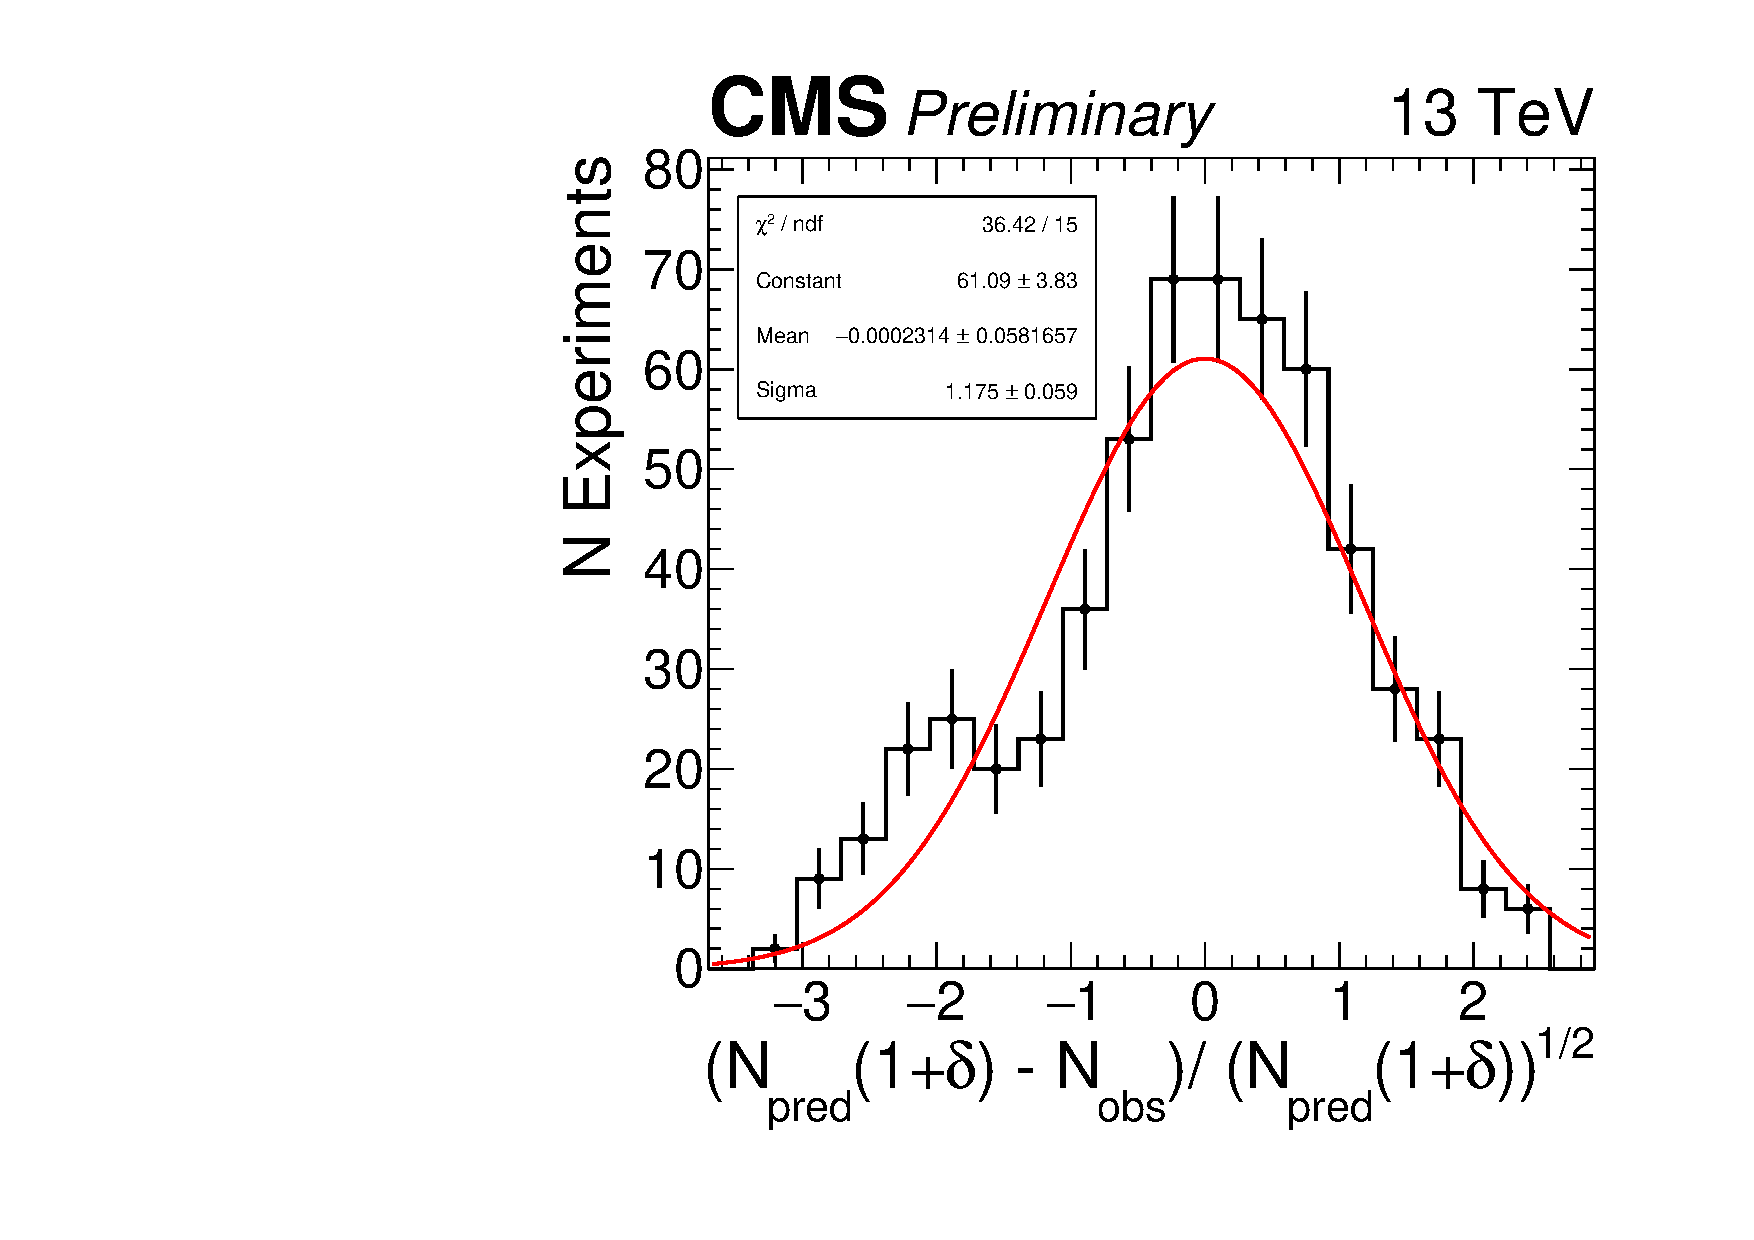
\includegraphics[width=.31\textwidth]{figures/an/ANALYSIS/pulls/data_loose_corrected_delta0p075_2tag.pdf}
\caption{Cross validation of the predicted of the number of baseline tags in data collected by the displaced jet triggers. Pulls for the 2 tag bin with the loose tag (left). Pulls with the signal region removal correction applied (middle). The same signal region removal correction shifted by $\delta=7.5\%$  (Right). 
\label{fig:djetpd_2tag_xval}}
\end{center}
\end{figure}


We summarize the cross validation studies in the following figures:
\begin{itemize}
\item Fig \ref{fig:djetpd_1tag_xval}: SR corrected and uncorrected 1 tag bin pulls for the Loose tag definition in Data collected by Displaced Jet Triggers. $N_{div}=25$
\item Fig \ref{fig:djetpd_1tag_xval_baseline}: SR corrected 1 tag bin pulls for the Baseline tag definition in Data collected by Displaced Jet Triggers. $N_{div}=25$
\item Fig \ref{fig:qcd_1tag_xval}: 1 tag bin pulls for the Loose tag definition in QCD events passing the Displaced Jet Triggers. $N_{div}=25$
\item Fig \ref{fig:qcd_2tag_xval}: 2 tag bin pulls for the Loose tag definition in QCD events passing by Displaced Jet Triggers. $N_{div}=25$
\item Fig \ref{fig:djetpd_2tag_xval}: SR corrected, uncorrected, and SR corrected+$\delta$ 2 tag bin pulls for the Loose tag definition in Data collected by Displaced Jet Triggers. $N_{div}=25$
\end{itemize}

In data and QCD, the SR correction provides a significant improvement on the pull distributions with respect to the ideal parameters $\mu=0$ and $\sigma=1.0$. For the 1 tag prediction in data with the loose tag the central value changes from $\mu=3.5$ (uncorrected) to $\mu=0.36$ (corrected). For the signal region (2+ tags), the loose tag in data is within 7.5\% of ideal $\mu$ and the QCD estimate is within error of $\mu=0$ but has $\sigma=1.6>1.0$. 

%% The 1 tag pulls for both the baseline and loose tag definitions have a mean constient with 0. The level of consistency is at 1 $\sigma_{mu}$ and 2.1 $\sigma_\mu$ for the baseline and loose tag definitions respectively. The purely poission 
%% error predicts  pulls with $\sigma_{gaus}=1$. For the baseline and loose tag definitions we have $\sigma_{gaus} = 1.33$ and $1.21$ respectively.
%% The fact these are greater than 1 is due to inaccuracies in the prediction method as well as the statistical uncertainty in the fake rate measurement. 


\section{Systematic uncertainties}
\label{sec:sys}

\subsection{Background systematic uncertainties}
\label{sec:bkgsys}

A background systematic uncertainty is quoted for the data-driven background prediction
method. This uncertainty is estimated by repeating the
background-prediction procedure on data with a looser version of the
displaced-jet tagging algorithm as outlined in section \ref{sec:bkg}.  The
background estimation uncertainty of 7.5\% is the required adjustment
to the prediction to remove the bias observed in the Gaussian fit.  For three or more tags, the systematic uncertainty for the
method is kept fixed.

The statistical uncertainty on the measured misidentification rate as a
function of $N_{\textrm{tracks}}$ is propagated to the predicted
$N_{\textrm{tags}}$ distribution as a systematic uncertainty. This systematic uncertainty 
is calculated for each tag multiplicity bin individually. The uncertainty for the 2 tag
bin is ${-}12$/$+13$\%.

In summary, for the background prediction in the two tag bin, a 7.5\% uncertainty is assigned to the
background prediction method and ${-}12$/$+13$\% uncertainty is assigned to 
the statistics of the misidentification rate. 

\subsection{Signal systematic uncertainties}
\label{sec:sigsys}
A summary of the systematic uncertainties associated with the signal
yields is given in Table~\ref{tab:sigSys}.  The uncertainty on the
trigger emulation is measured by comparing the predicted efficiency
for simulated multijet events and data collected by a loose
$H_{\textrm{T}}$ trigger. The observed difference at threshold (5\%)
is taken as an estimate of the uncertainty in the emulation of the
online $H_{\textrm{T}}$ requirement.  Similarly, the uncertainty
induced by the online versus offline jet acceptance is obtained from
the shift in the trigger efficiency when the offline jet $p_{t}$
requirement is increased from $p_{t}>60$ GeV to $p_{t}>80$ GeV (5\%).

The systematic uncertainty on the luminosity is 2.7\% \cite{LUMI}.


\begin{figure}
\begin{center}
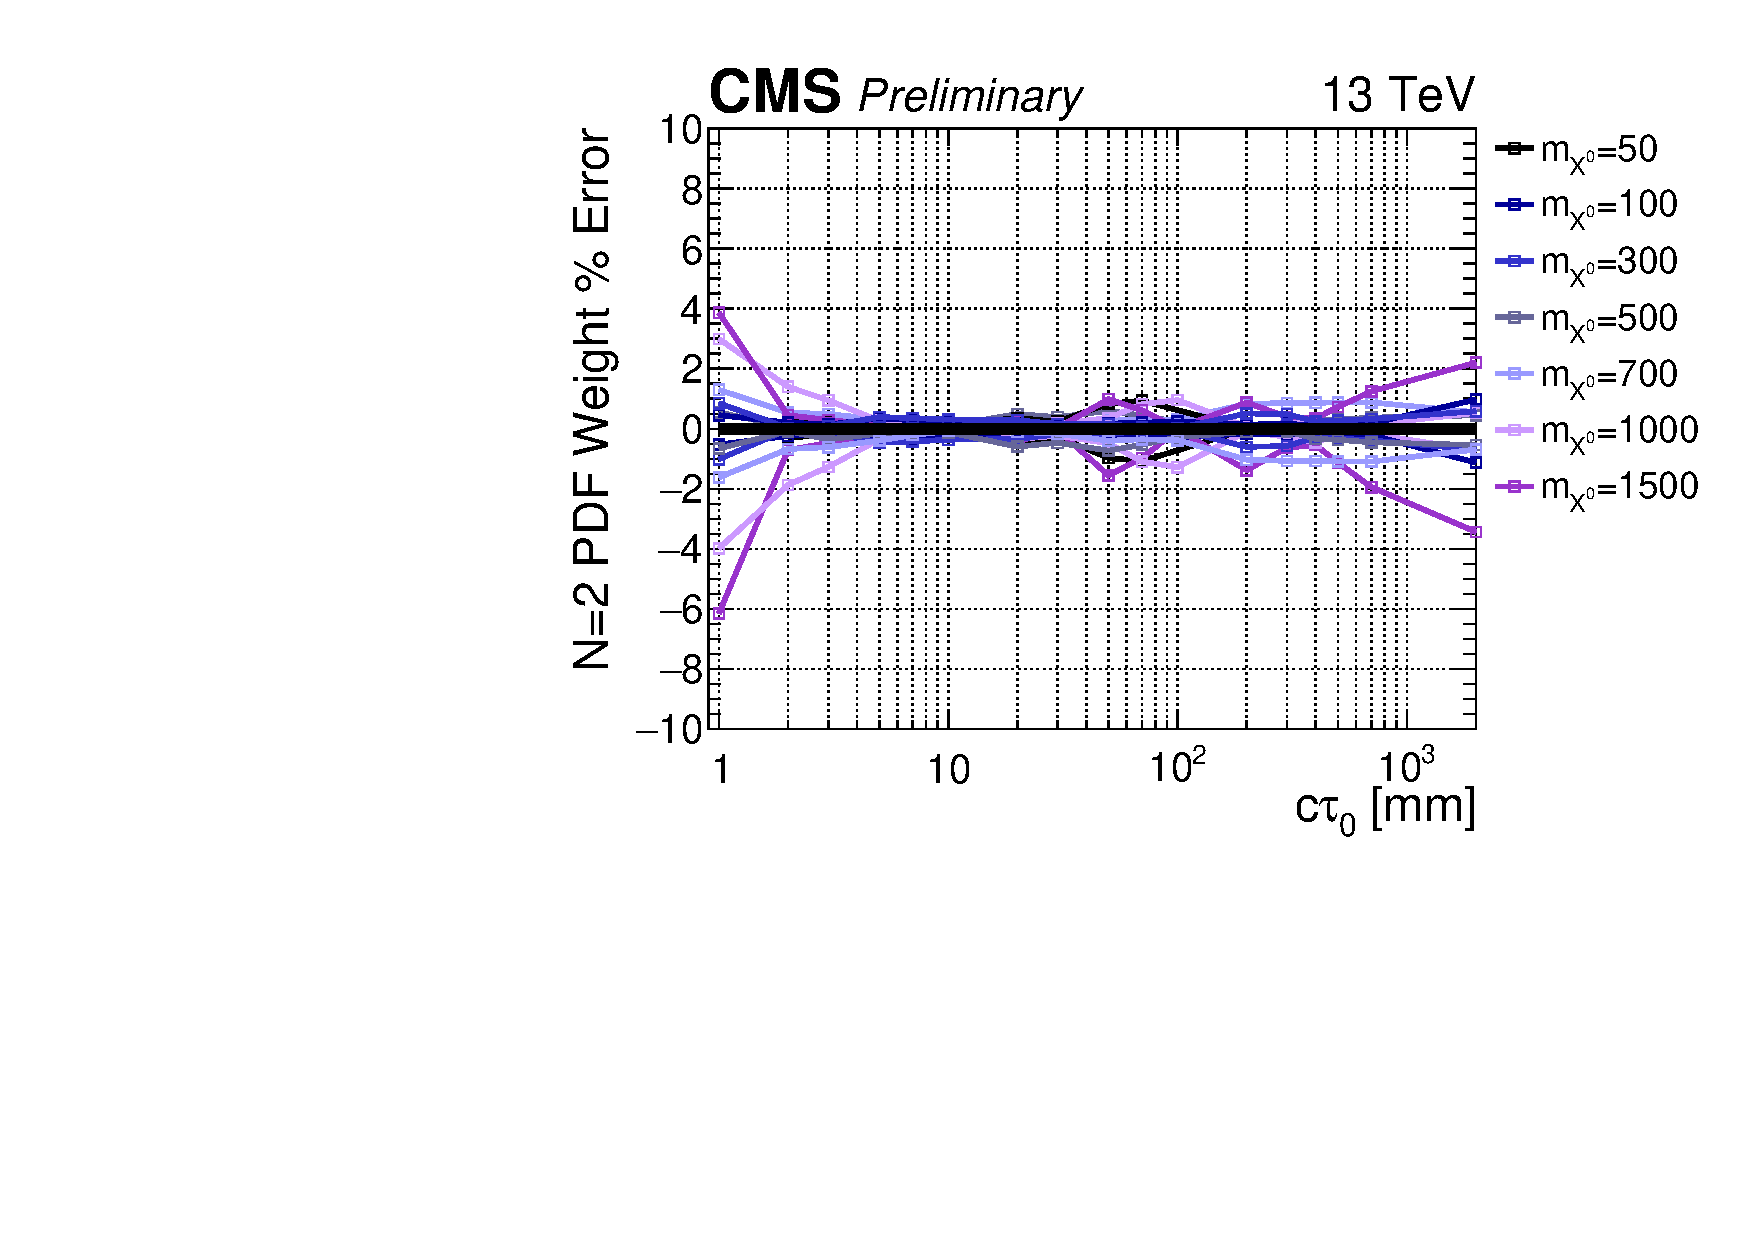
\includegraphics[width=.45\textwidth]{figures/an/SYSTEMATICS/76x_pu/sys_2tag_pdf.pdf}
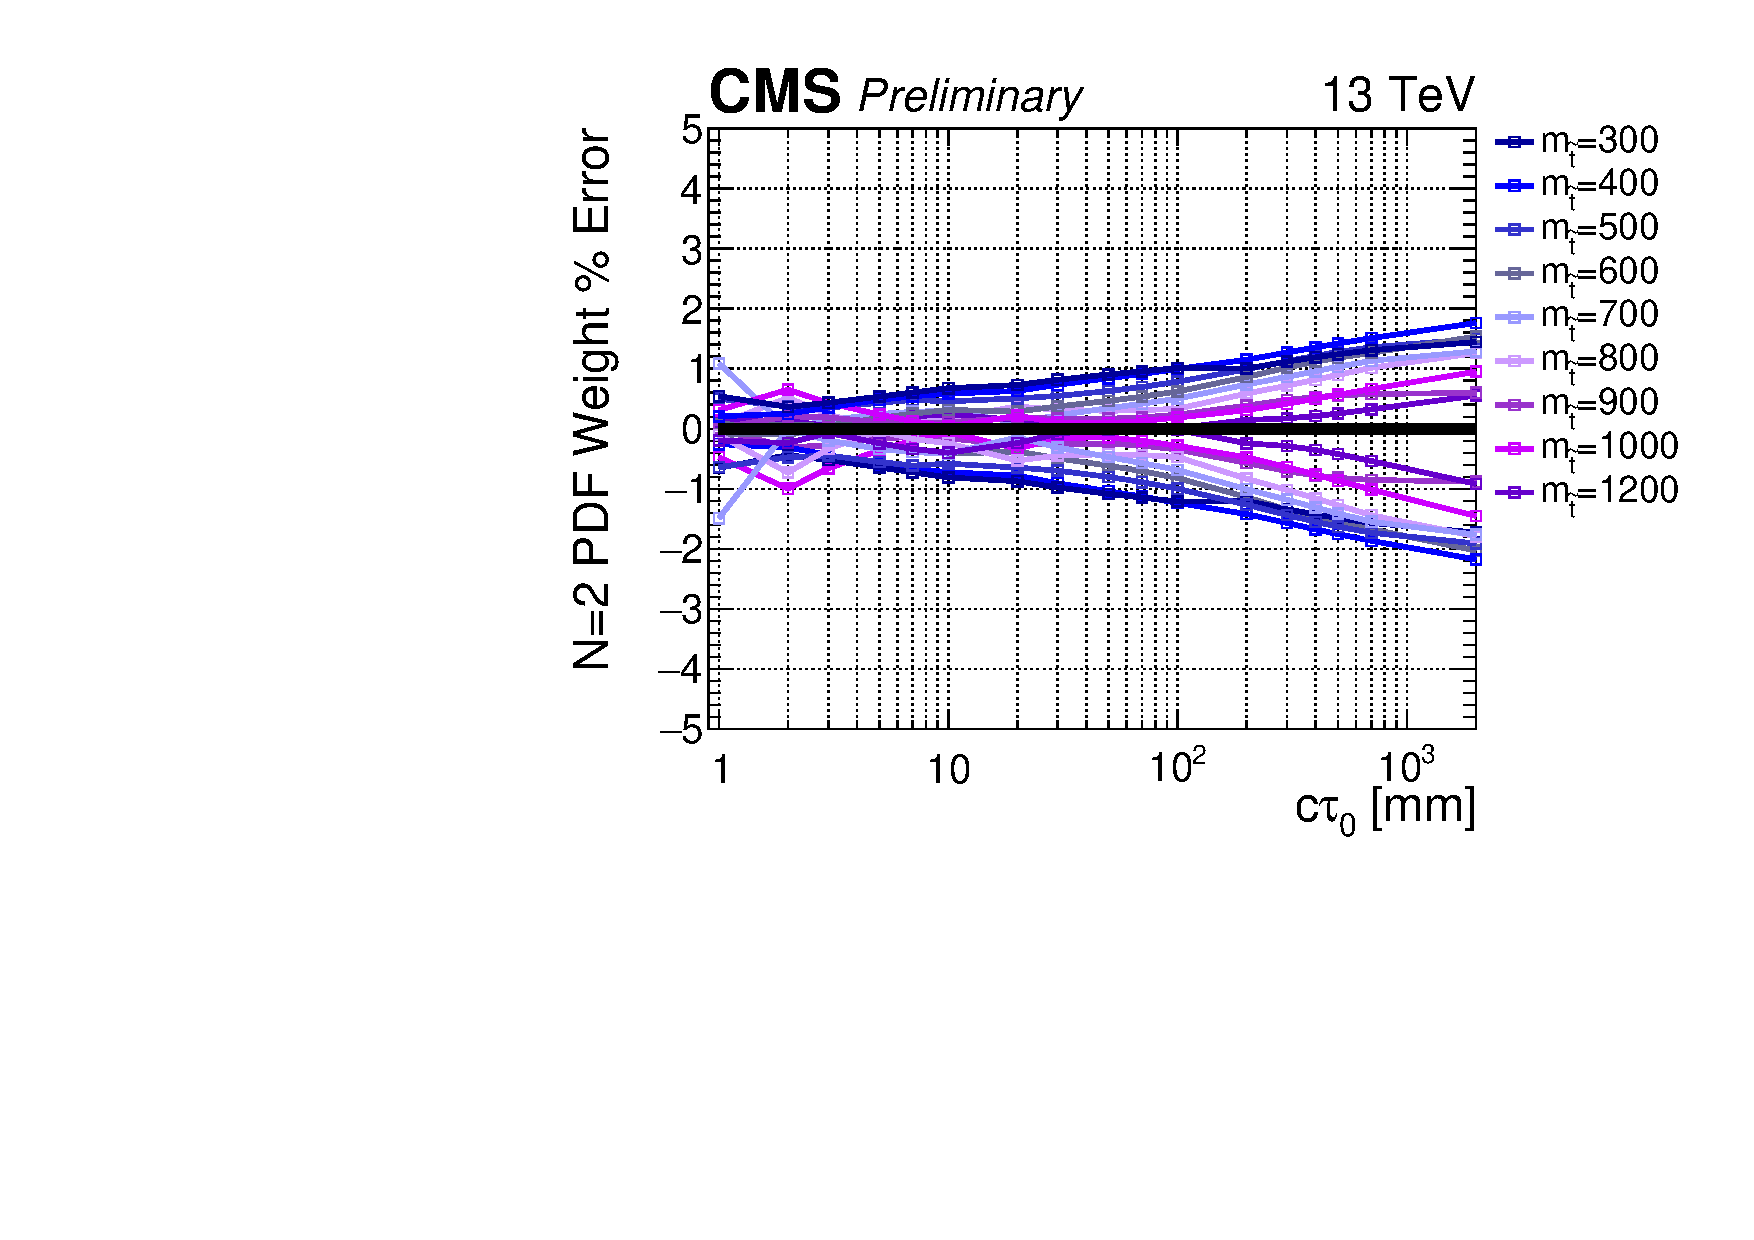
\includegraphics[width=.45\textwidth]{figures/an/SYSTEMATICS/76x_pu/sys_2tag_pdf_dsusy.pdf}
\caption{The PDF acceptance  systematics in the Jet-Jet (left)
 and B-Lepton (right) signal model as a function of the mass $m_X$ 
or $c\tau_0$ for the 2 tag bin. The systematic is reported two sided 
for the two tag bin in the analysis. The error to fluctuate up is in
 the upper half plane and the error to fluctuate down on the lower half plane.  \label{fig:pdf_sys}}
\end{center}
\end{figure}

The uncertainty arising from the PDFs for pair-produced masses in the
range of 50--1500GeV is found to be 1--6\% Figure \ref{fig:pdf_sys}.  An ensemble of
alternative PDF is sampled from the output of the NNPDF fit.  Events
are reweighted according to the ratio between these alternative PDF
sets and the nominal ones. The distribution of the signal prediction
for these PDF ensemble is used to quantify the uncertainty.

\begin{figure}
\begin{center}
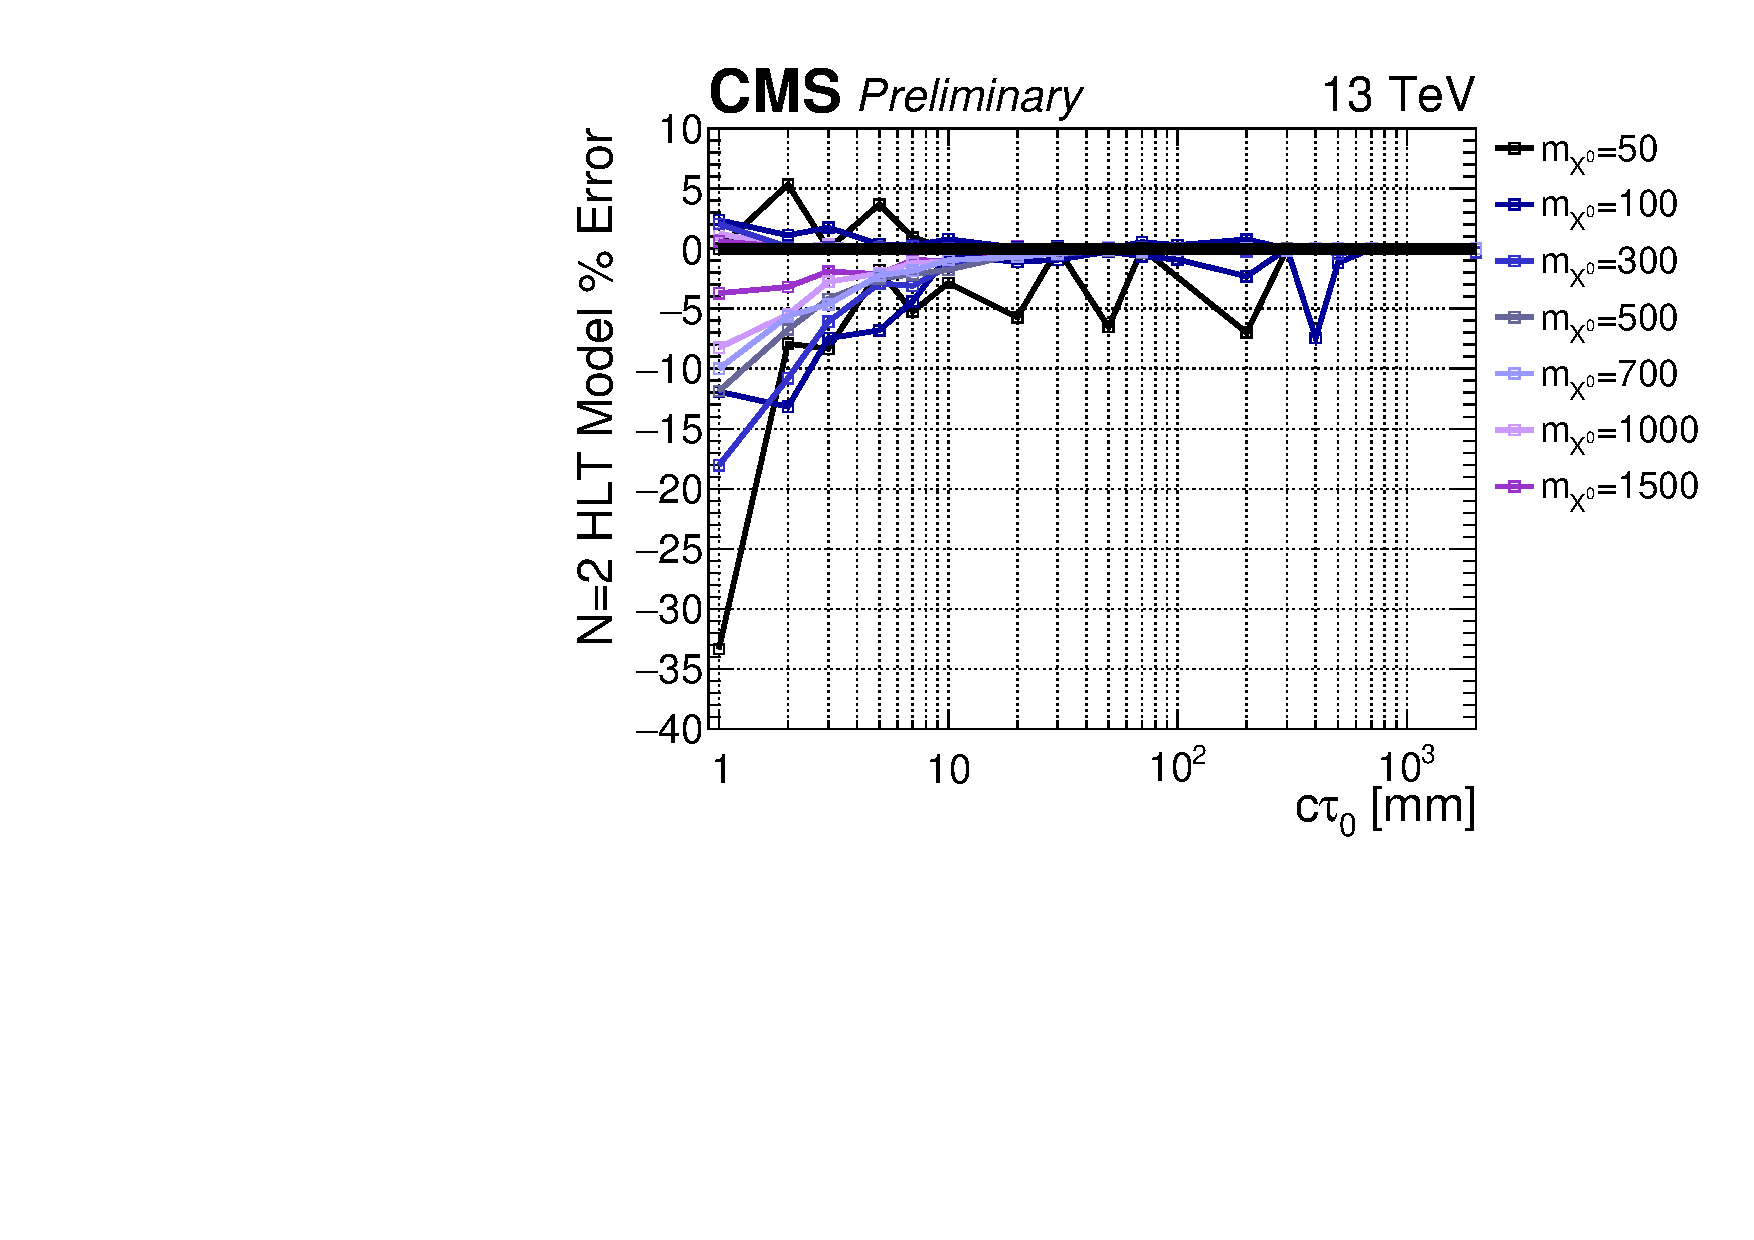
\includegraphics[width=.45\textwidth]{figures/an/SYSTEMATICS/76x_pu/sys_2tag_hlt.pdf}
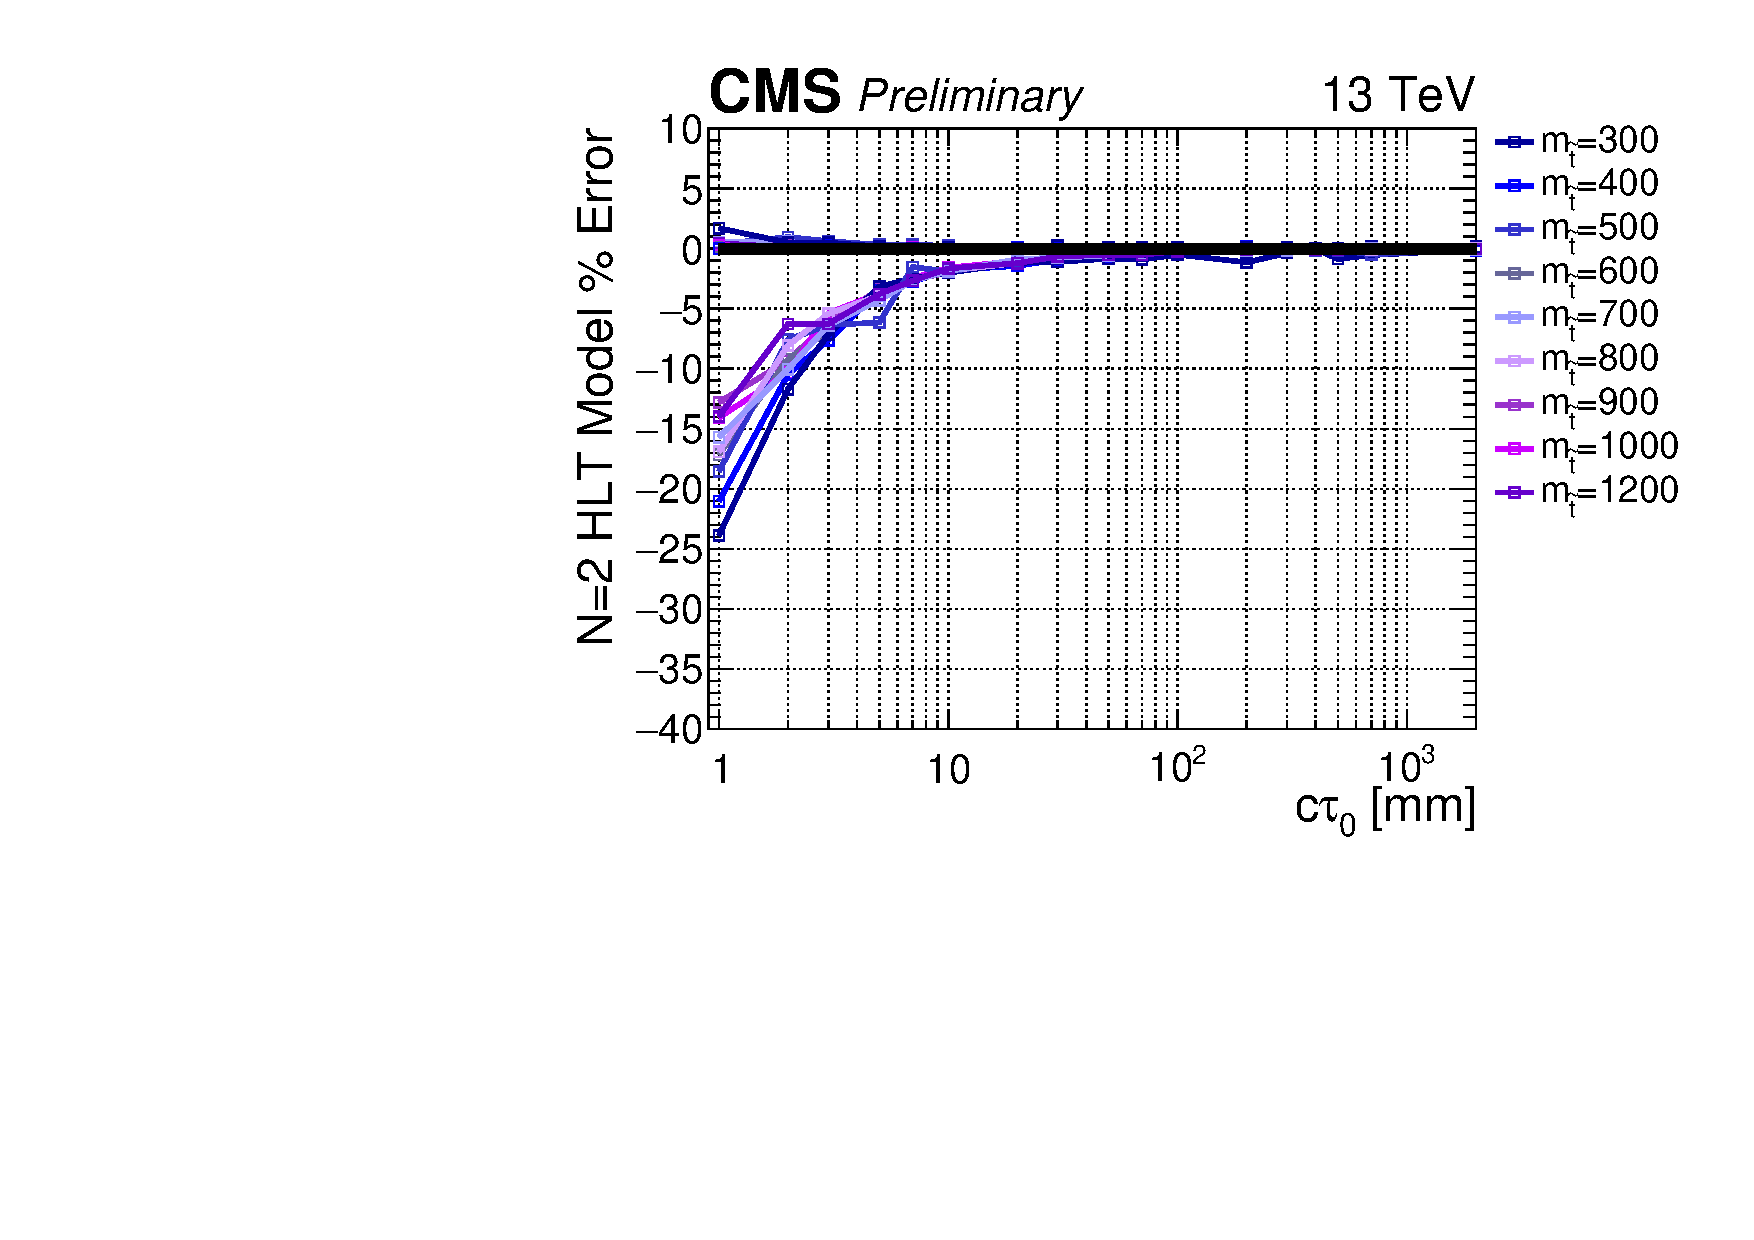
\includegraphics[width=.45\textwidth]{figures/an/SYSTEMATICS/76x_pu/sys_2tag_hlt_dsusy.pdf}
\caption{The onling tracking related systematics in the Jet-jet (left ) and B-Lepton
 (right )  model as a function of $c\tau_0$. (Top) The online track 2DIP and
 2DIP$_{sig}$ modeling in the 2 tag bin   \label{fig:online_tracking_sys}}
\end{center}
\end{figure}

\begin{figure}
\begin{center}
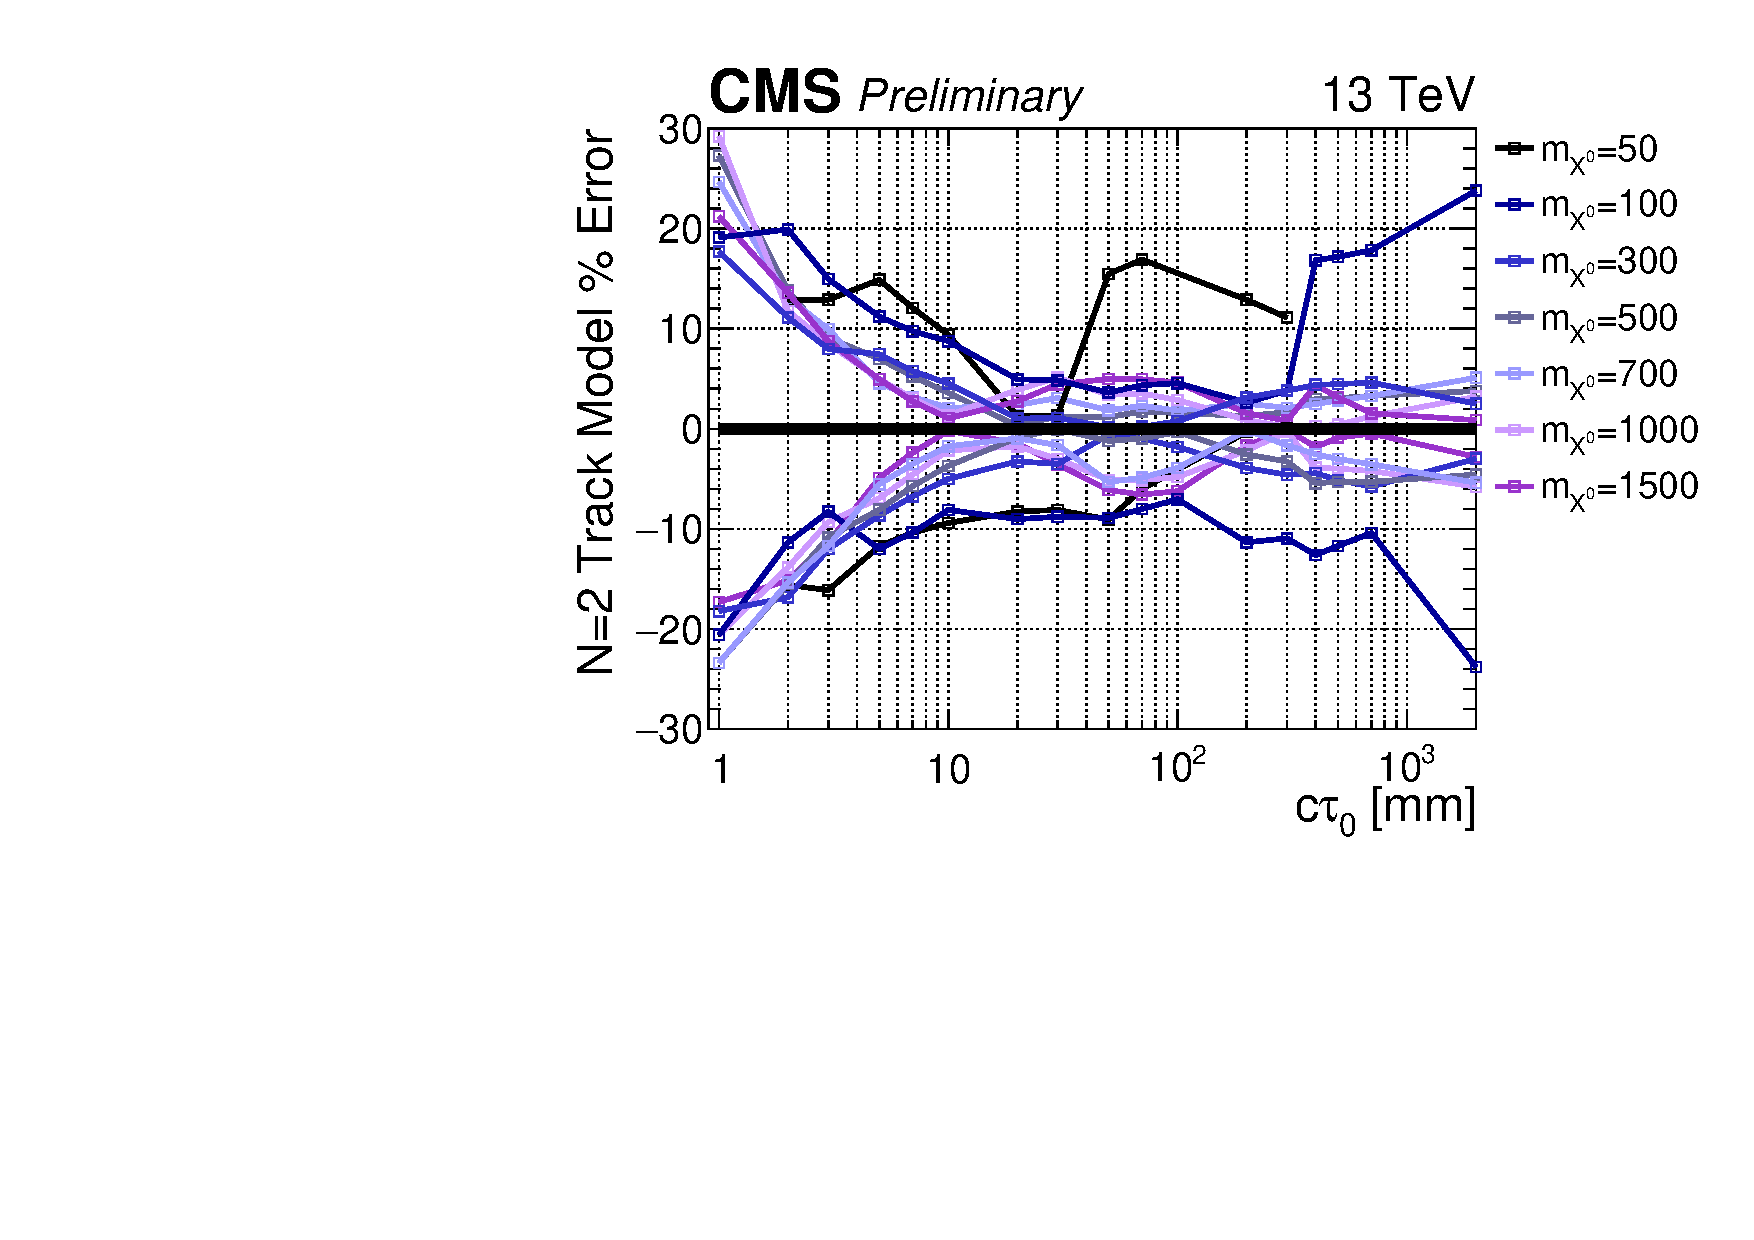
\includegraphics[width=.45\textwidth]{figures/an/SYSTEMATICS/76x_pu/sys_2tag_tracking.pdf}
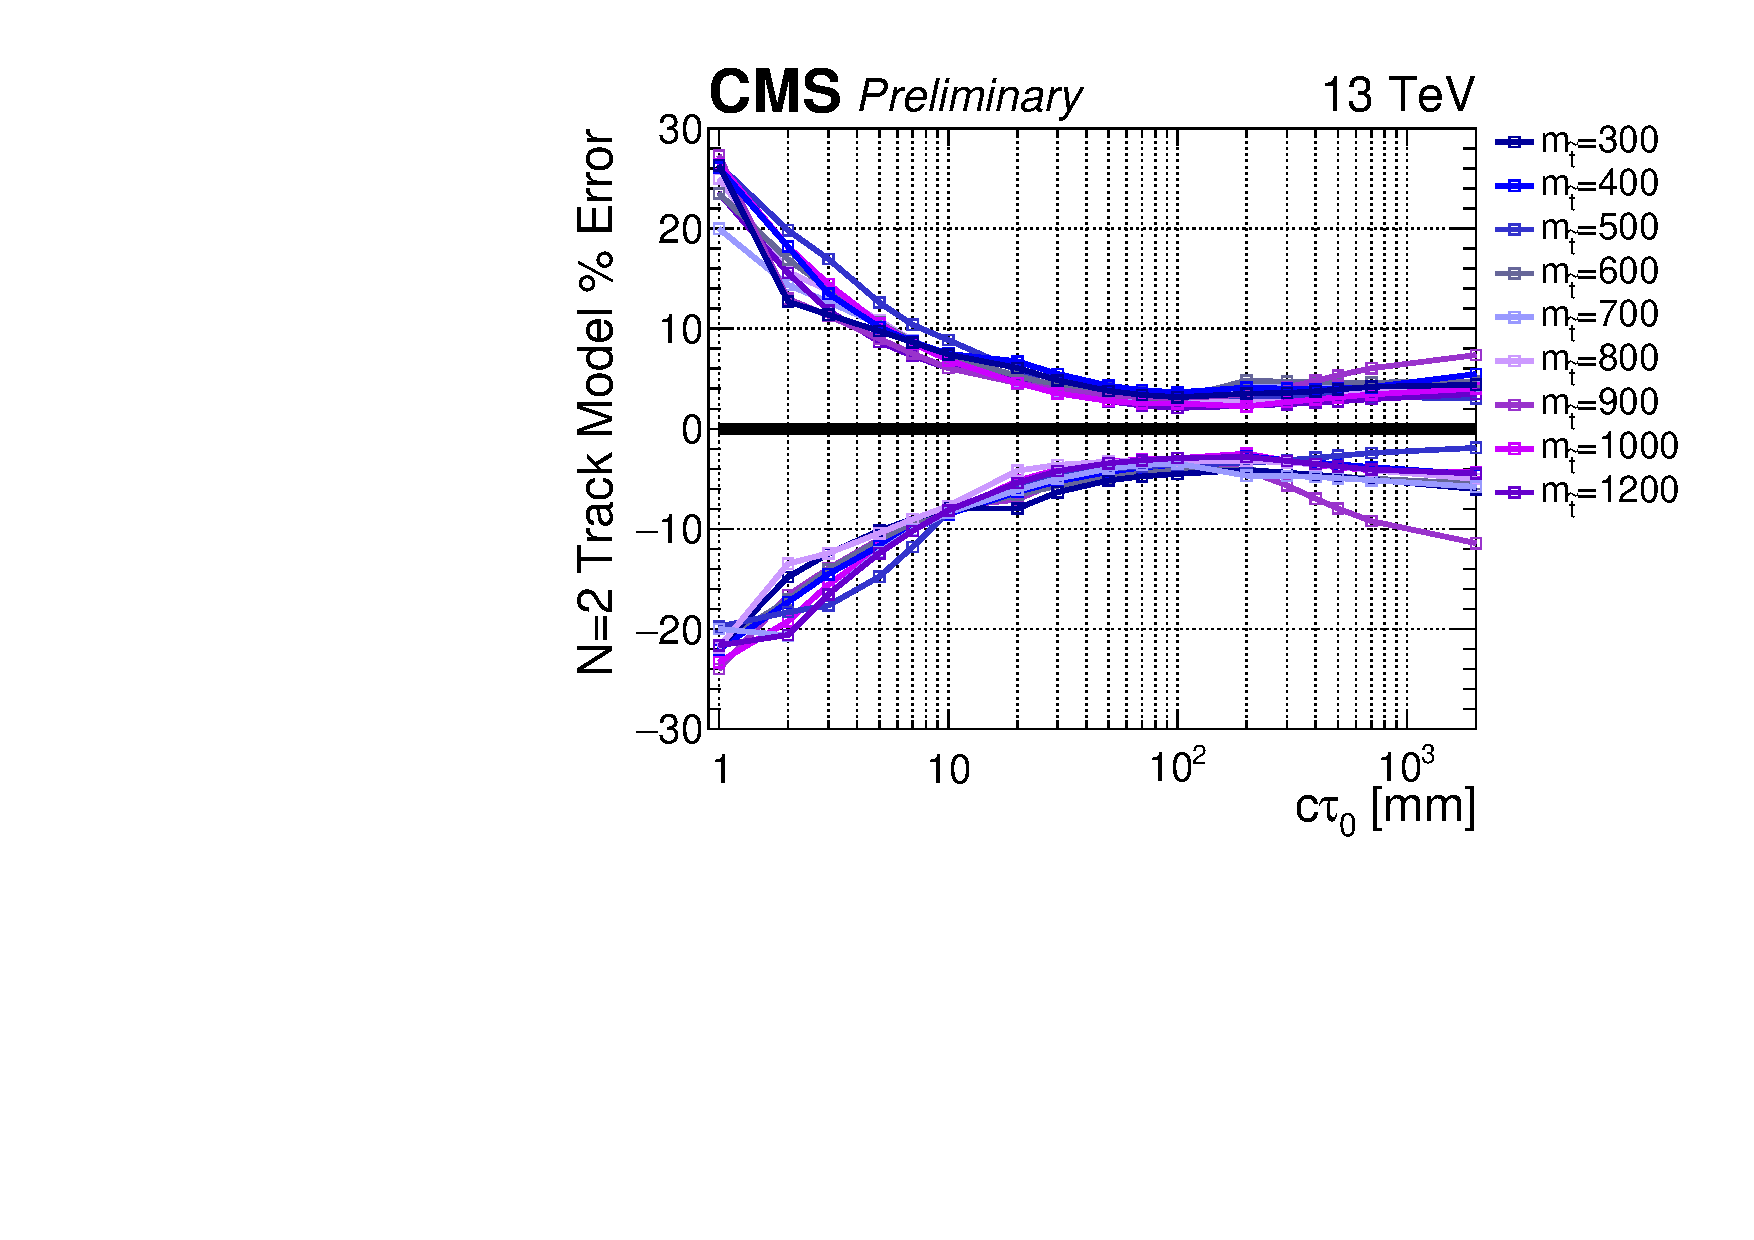
\includegraphics[width=.45\textwidth]{figures/an/SYSTEMATICS/76x_pu/sys_2tag_tracking_dsusy.pdf}
\caption{The two tracking related systematics in the Jet-Jet (left ) and B-Lepton
 (right )  model as a function of $c\tau_0$.  The displaced jet tagging variable 
systematic in the 2 tag bin. The systematic is reported two sided for the two tag
 bin in the analysis. The error to fluctuate up is in the upper half plane and the
 error to fluctuate down on the lower half plane.  \label{fig:offline_tracking_sys}}
\end{center}
\end{figure}

The systematic uncertainty on the modeling of the jet tagging
variables in signal MC samples is estimated from the displaced track
modeling in multi-jet events in data and MC. The mismodeling of the
measured value of $\Theta_{\textrm{2D}}$ and $IP_{\textrm{sig}}^{\textrm{2D}}$ for
single tracks is propagated to the final tag distribution by varying
the individual measured values in MC by the difference in the measured
value relative to data (3--10\%). The tagging variables are then
re-calculated.  The $N_{\textrm{tags}}$ distribution is recalculated
with the new values. The systematic uncertainty is assigned as the
relative change in events, bin by bin in $N_{\textrm{tags}}$. For the
two tag bin, this varies from 1 to 30\% depending on the mass and
lifetime Figure \ref{fig:offline_tracking_sys}. The mismodeling of
 $\alpha_{\textrm{max}}$ is found to have a negligible effect on the
 signal efficiency as the requirement is relatively loose.

The systematic uncertainty on the modeling of the online tracking
efficiency is obtained by studying the online regional track
reconstruction in data and MC. The online values of $IP^{\textrm{2D}}$
and $IP^{\textrm{2D}}_{\textrm{sig}}$ are varied by the magnitude of
the mismodeling found in events collected in control triggers.  The
new values are used to determine if the event would still pass at
least one of the trigger paths and its associated offline
$H_{\textrm{T}}$ requirement. The $N_{\textrm{tags}}$ distribution is
recalculated with the values varied up and down. The relative change
in the number of events per bin is taken as the systematic
uncertainty. For the two tag bin, this uncertainty varies from
1 to 35\%.

All signal systematic uncertainties are calculated individually for
each model for all individual mass and lifetime points, and for each
value of $N_\text{tags}$ in the signal region.



\begin{table}[tb]
  \caption{Summary of the systematic uncertainties. 
    When the uncertainty depends on the specific features of the models
    (mass, lifetime and decay mode of the long-lived particle) a
    range is quoted, which refers to the computed uncertainty for $N_{\textrm{tags}}=2$ events.~\label{tab:sigSys}}
\begin{center}
\begin{tabular}{cc}
\textbf{Signal systematic uncertainty} & \textbf{Effect on yield} \\
\hline
$H_{\textrm{T}}$ trigger inefficiency &  5.0\% \\
Jet $p_{t}$ trigger inefficiency  & 5.0\% \\
Trigger online tracking modeling & 1.0--35.0\% \\
Luminosity & 2.7\% \\
Acceptance due to PDF & 1.0--6.0\% \\
Displaced-jet tag variable modeling & 1.0--30.0\% \\
\end{tabular}
\end{center}
\end{table}

\section{Results and interpretation}
\label{sec:results}

\begin{table}[tb]
  \caption{The predicted and observed number of events as a function
    of $N_{\textrm{tags}}$. The prediction is based on the
    mistagging probability derived from events with fewer than two tags. 
    The full event selection is applied. The quoted uncertainty
    corresponds to the total background systematic uncertainty.\label{tab:result}}
\begin{center}
\begin{tabular}{ccc}
\textbf{$N_{\textrm{tags}}$} & \textbf{Expected} & \textbf{Observed} \\
\hline
2 & $1.09^{+0.16}_{-0.15}$ & 1  \\
$\geq~3$ & $(4.9 \pm 1.0) \times 10^{-4}$ & 0 \\
\end{tabular}
\end{center}
\end{table}

The numerical values for the expected and observed yields are
summarized in Table ~\ref{tab:result}.  The observed yields are found to
be consistent with the predicted background, within the statistical
and systematic uncertainties. No evidence for a signal at large values
of $N_{\textrm{tags}}$ is observed. 

Exclusions for each model are obtained from the predicted and observed
event yields in Table~\ref{tab:result} and the signal efficiencies in
Tables~\ref{tab:cutflow_30mm}--\ref{tab:cutflow_BR_mass}.  All bounds
are derived at 95\% confidence-level (CL) according to the CL$_{s}$
prescription~\cite{CLs1,CLs2,LHCCLs} in the asymptotic approximation.
For each limit derivation, we consider events with $N_{\textrm{tags}}\geq 2$ 
using independent bins for $N_{\textrm{tags}}=2$ and
$N_{\textrm{tags}}\geq 3$. Finer binning of the tag multiplicity for $N_{\textrm{tags}}>3$
is found to have a negligible affect on the expected limits. 
Cross section upper limits are
 presented as a function of the
mass and lifetime of the parent particle.  The analysis sensitivity is
maximal for $(10 < c\tau_0 < 1000)$mm. Mass exclusion bounds at
fixed lifetime are also derived, comparing the excluded cross section
with the values predicted for the benchmark models described in
section~\ref{sec:samples}. In the case of SUSY models, the
next-to-leading order (NLO) and next-to-leading-logs (NLL)
$\tilde{t}\tilde{t}$ production cross section is used as reference,
computed in the large-mass limit for all the other SUSY
particles~\cite{NLONLL1,NLONLL2,NLONLL3,NLONLL4,NLONLL5,NLONLLerr}.

Figures~\ref{fig:xx4j_limit}~and~\ref{fig:light_limit} show the
excluded pair-production cross section for the Jet-Jet and Light-Light
models, respectively. Cross sections as small as 1.2 fb are excluded
for $c\tau_0=50$mm for both models. 
Exclusion limits are also derived for resonances decaying to $b\ell$
final states, as shown in Fig.~\ref{fig:dsusy_limit_lepton}. The
sensitivity is similar to what is observed for the Jet-Jet model,
although less stringent as additional jets give higher efficiency than
additional leptons from both the tagging and triggering
perspectives. Cross sections larger than 2.47 fb are excluded at 95\%
CL, for $c\tau_0$ in the range $70$--$100$~mm excluding a
parent mass value of 1135~GeV.  

Figures~\ref{fig:dsusy_limit_tau}~and~\ref{fig:dsusy_limit_ele} show
the exclusions on the B-Tau and B-Ele models, respectively. The two
models have similar performance at high mass  with slightly stronger limits 
for the B-Ele model at lower
mass $m_{\tilde{t}}=300$~GeV and lifetimes $c\tau_0>10$mm. The
highest mass excluded in the B-Ele (B-Tau) model occurs at
$m_{\tilde{t}}=1150$ (1155)GeV and $c\tau_0=70$ (70)mm at an
observed cross section upper limit of 2.25 (2.17) fb at 95\% CL.

In contrast, Fig.~\ref{fig:dsusy_limit_mu} shows the exclusion for the
B-Mu model. Since the analysis uses jets reconstructed from
calorimetric deposits while the two muons have small or no associated
calorimeter deposit, the signal reconstruction efficiency and
displaced-jet multiplicity are smaller in this case. This results in a
weaker exclusion bound.  The highest mass excluded in the B-Mu model
occurs at $m_{\tilde{t}}=1090$~GeV and $c\tau_0=70$mm at an
observed cross section upper limit of 3.36 fb at 95\% CL.

\begin{figure}[tb]
\begin{center}

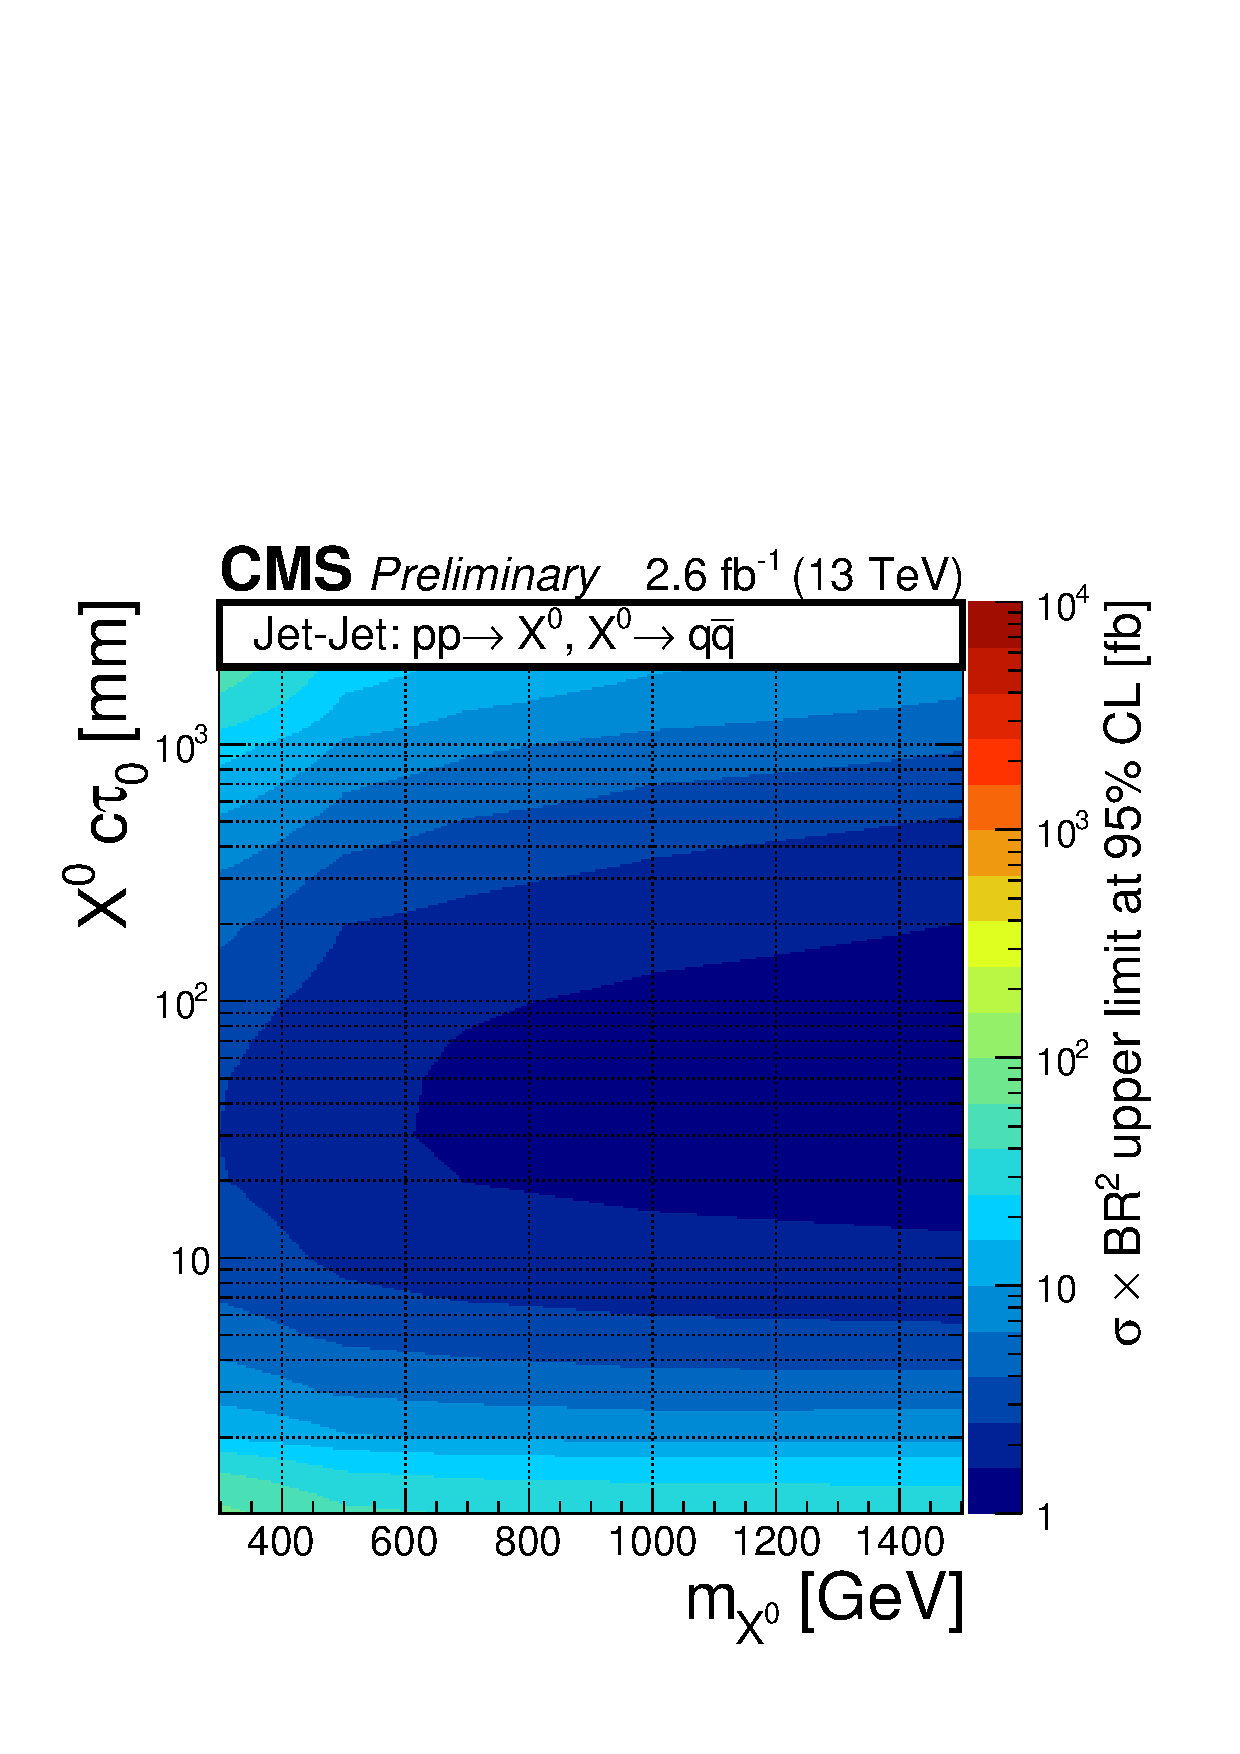
\includegraphics[width=.75\textwidth]{figures/pas//RESULT/UNBLINDED_LIMITS/Jet-Jet2D.pdf}
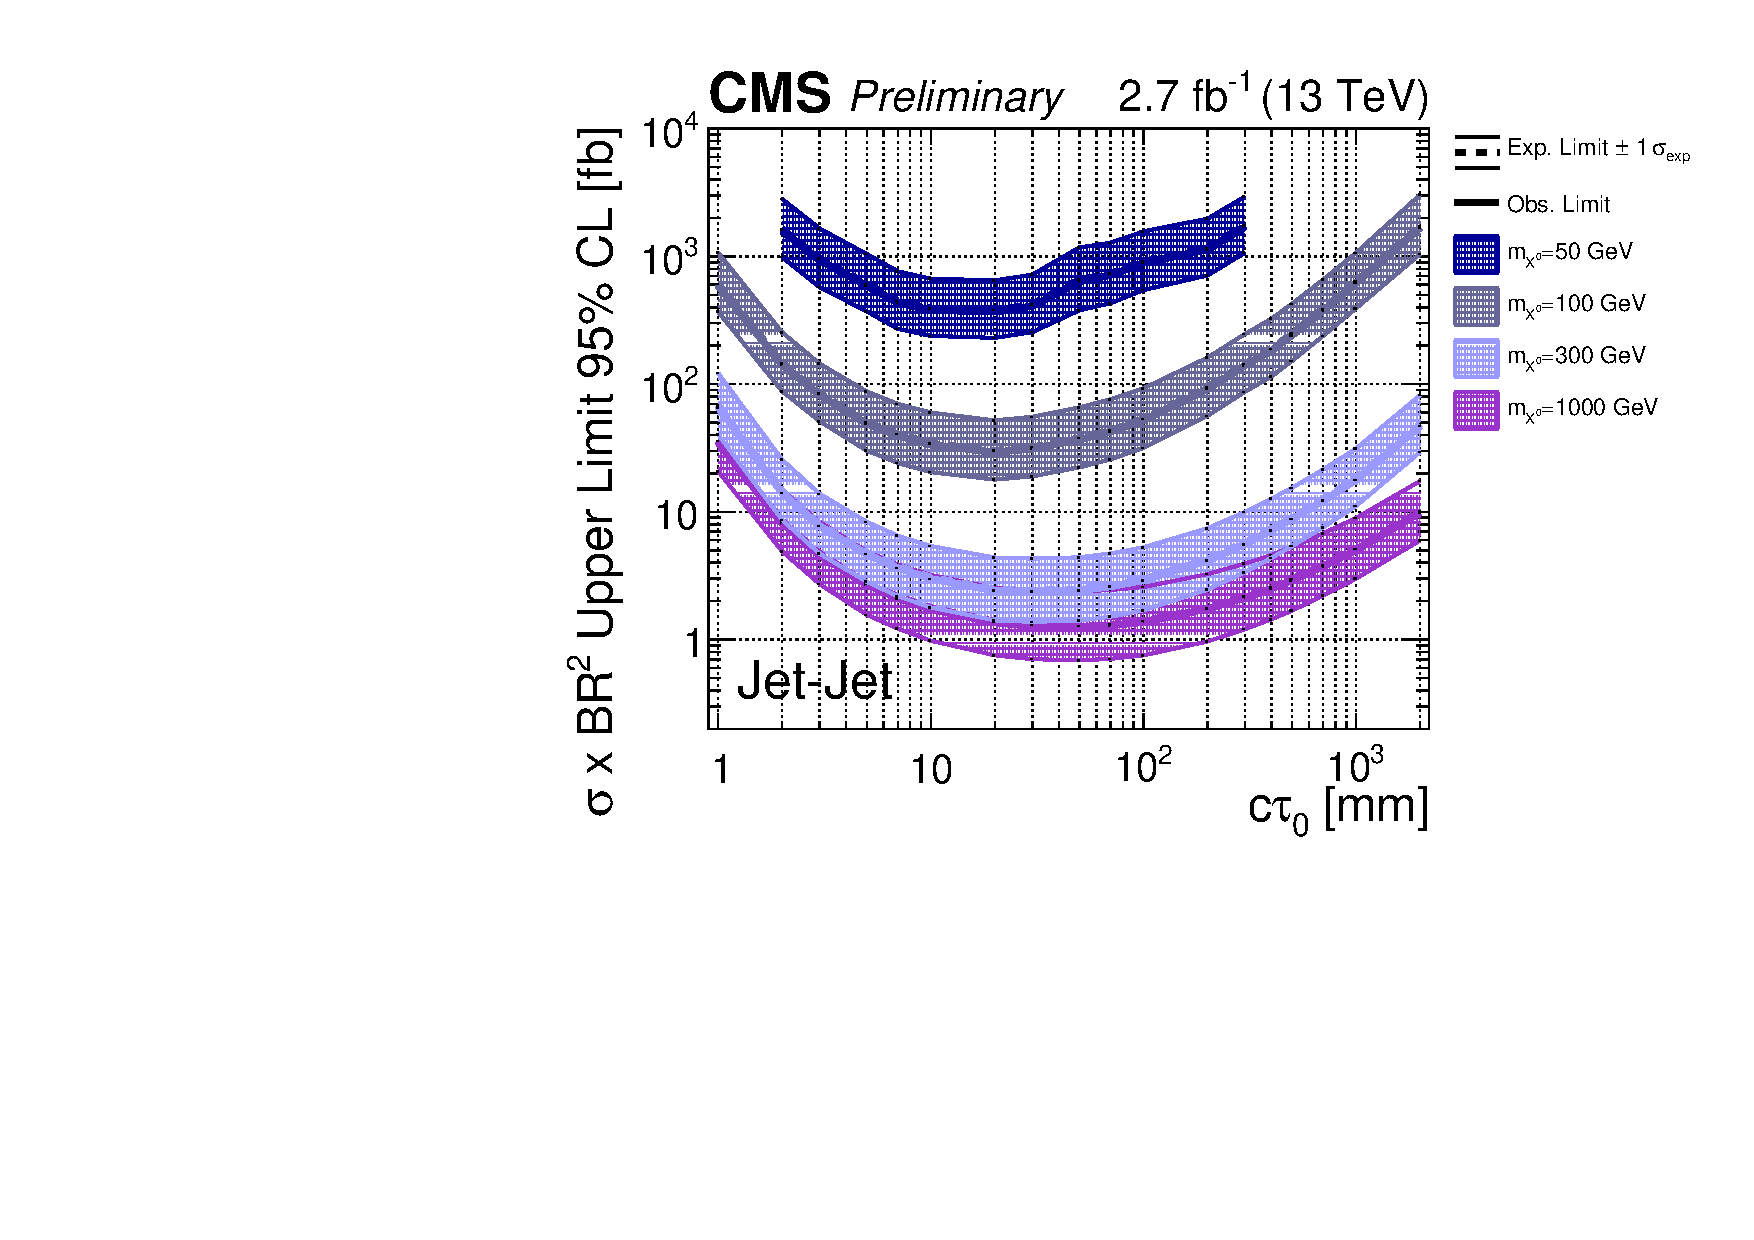
\includegraphics[width=.75\textwidth]{figures/pas//RESULT/UNBLINDED_LIMITS/Jet-Jet.pdf}
\caption{The excluded cross section at 95\% CL for the Jet-Jet model
  as a function of the mass and lifetime of the parent particle $X^0$
  (top) and as a function of the lifetime for four values of the mass
  (bottom).\label{fig:xx4j_limit}}
\end{center}
\end{figure}

\begin{figure}[tb]
\begin{center}
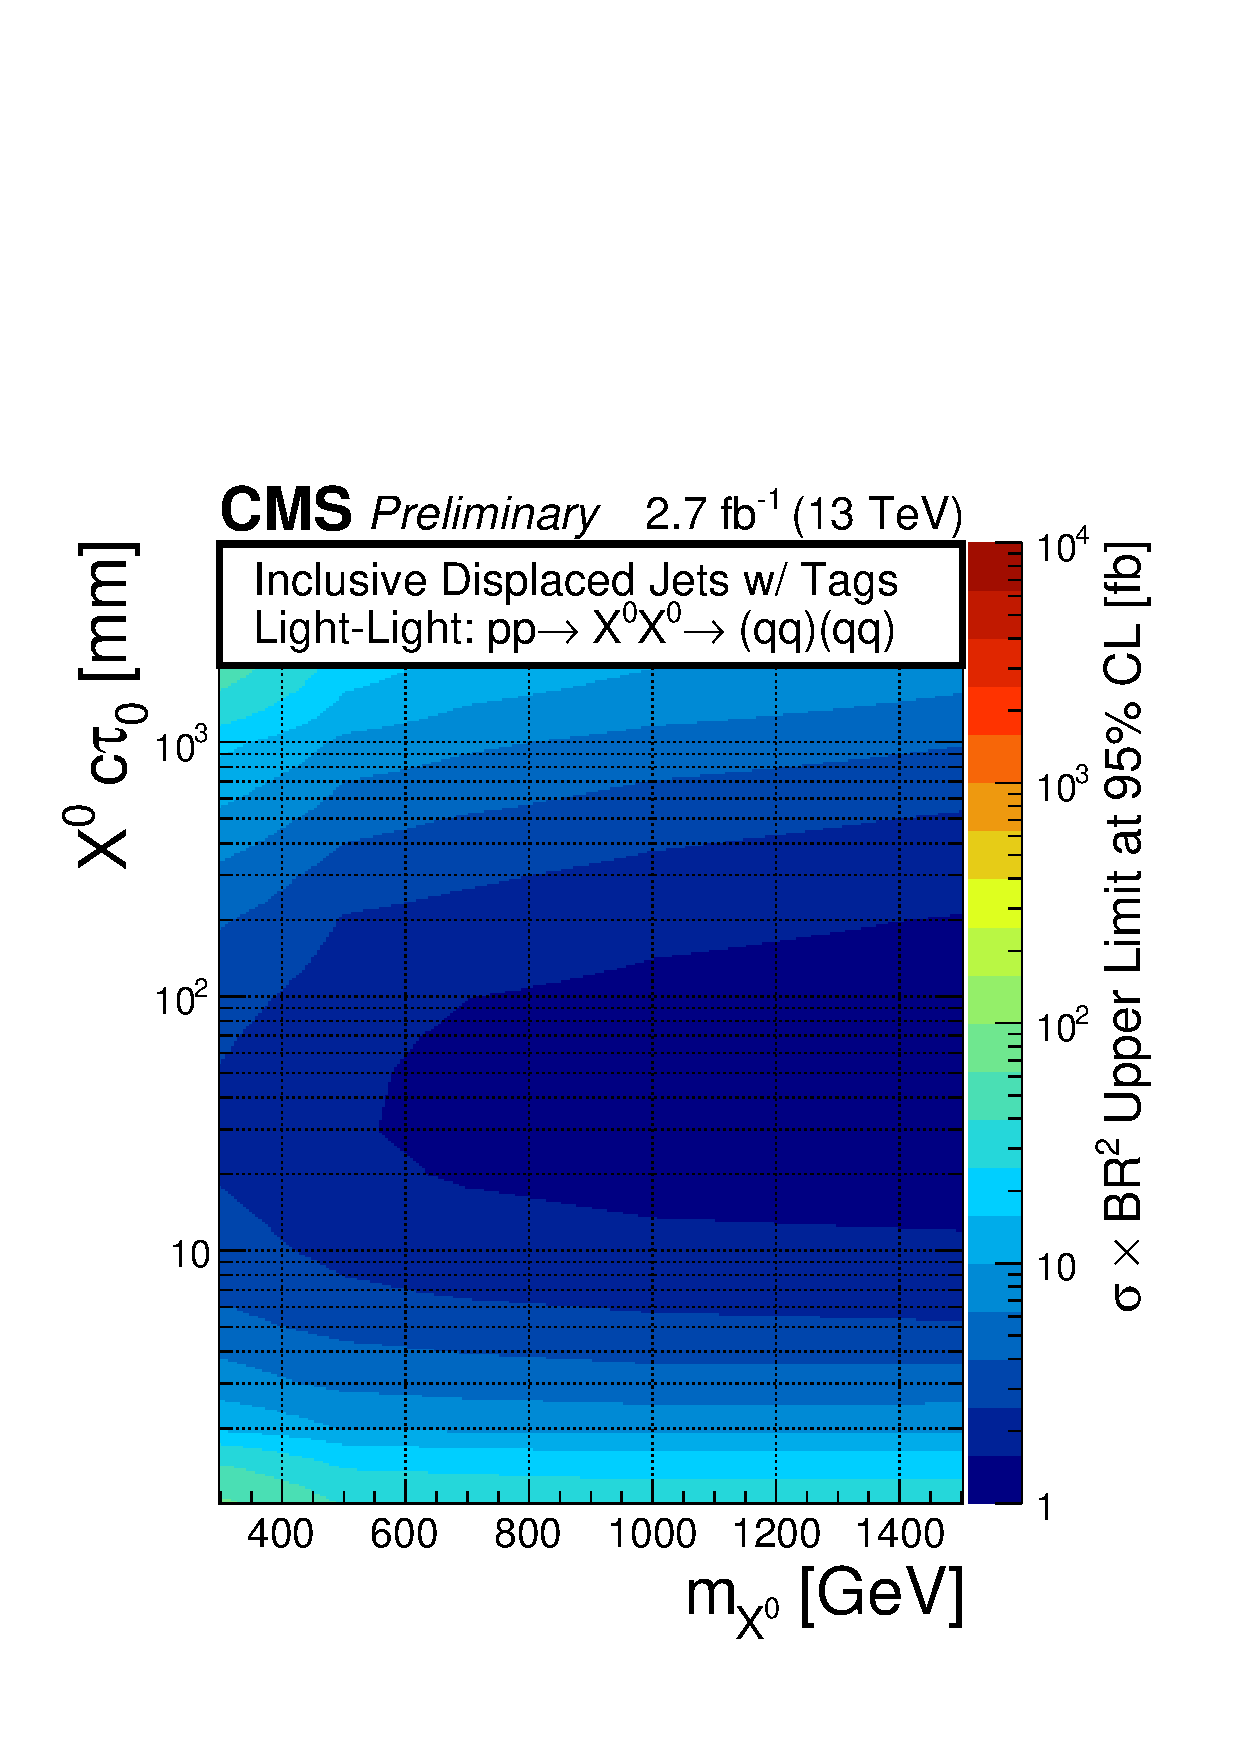
\includegraphics[width=.75\textwidth]{figures/pas//RESULT/UNBLINDED_LIMITS/Light-Light2D.pdf}
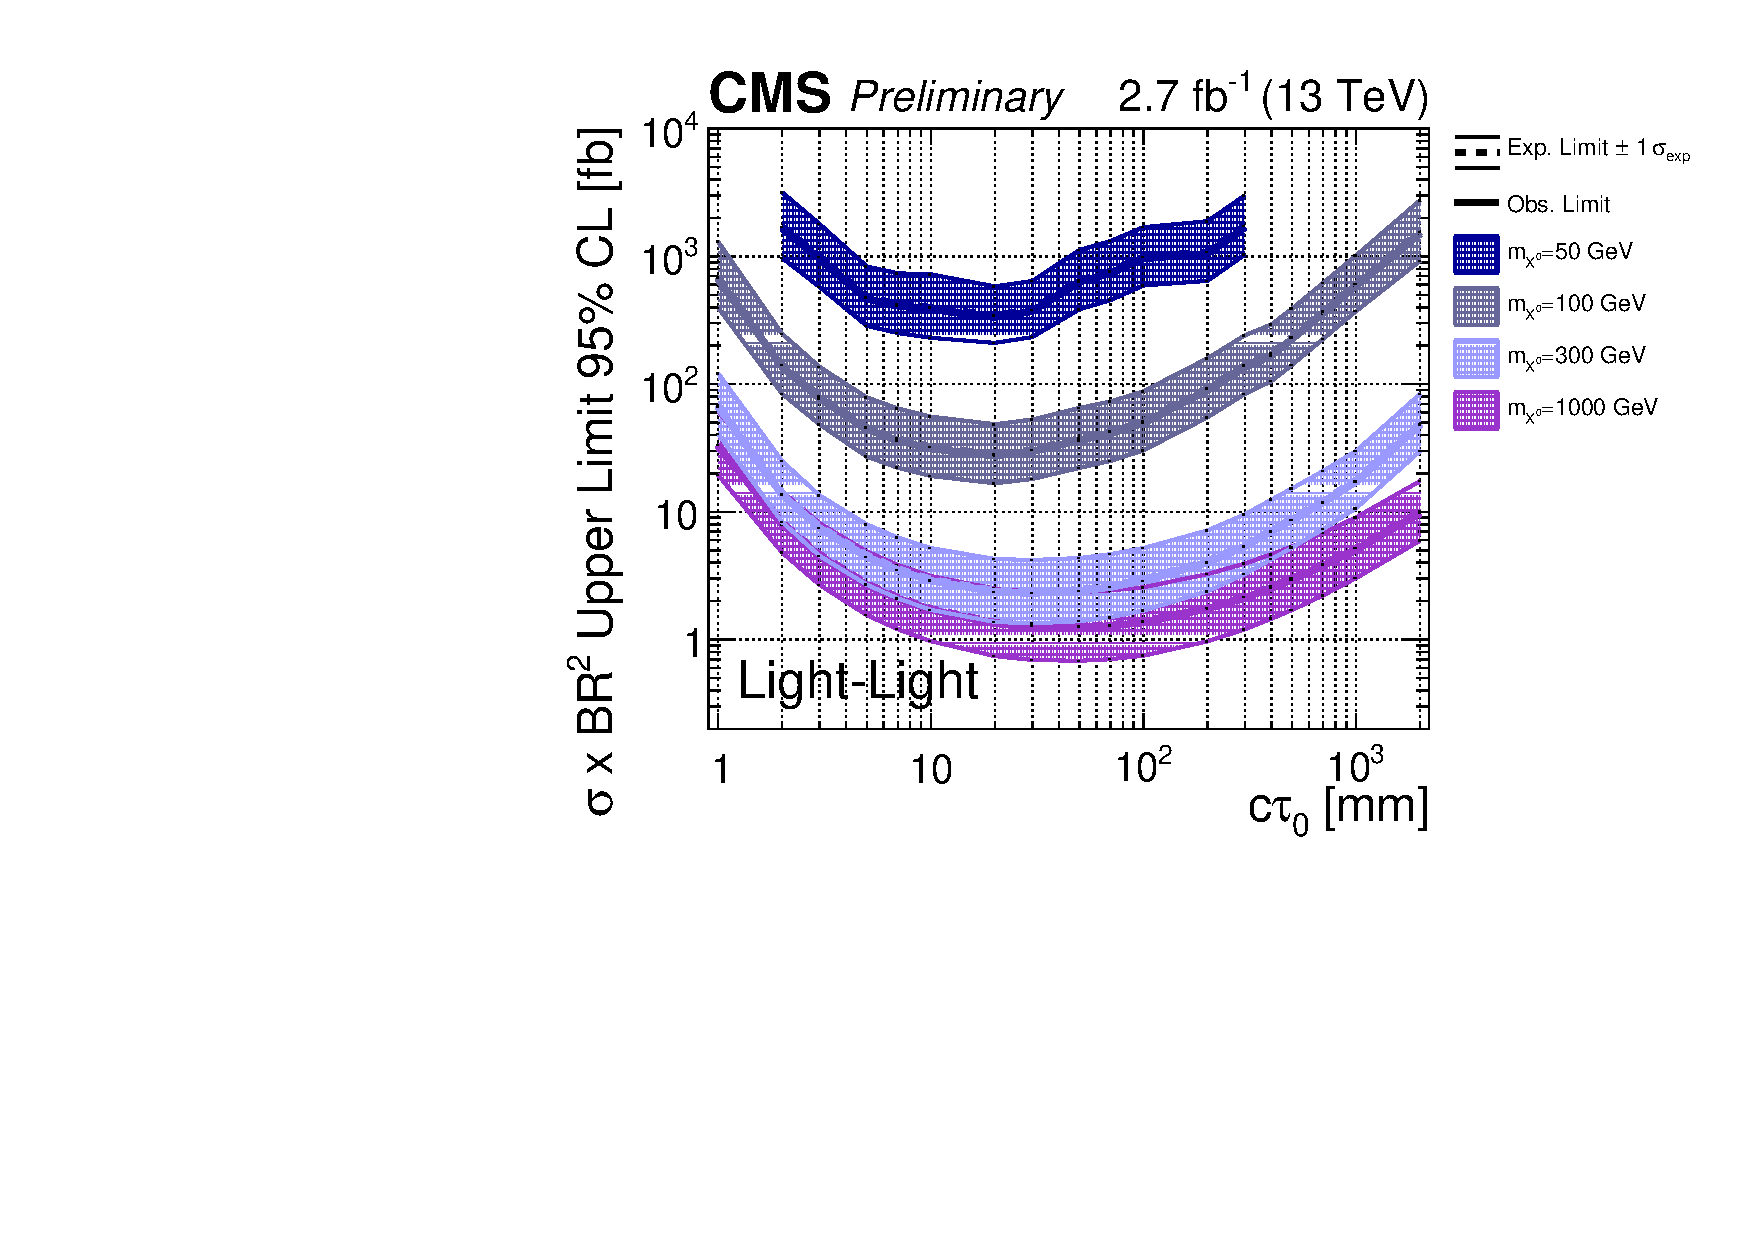
\includegraphics[width=.75\textwidth]{figures/pas//RESULT/UNBLINDED_LIMITS/Light-Light.pdf}
\caption{The excluded cross section at 95\% CL for the Light-Light
  model as a function of the mass and lifetime of the parent particle
  $X^0$ (top) and as a function of the lifetime for four values of the
  mass (bottom).\label{fig:light_limit}}
\end{center}
\end{figure}

\begin{figure}[tb]
\begin{center}
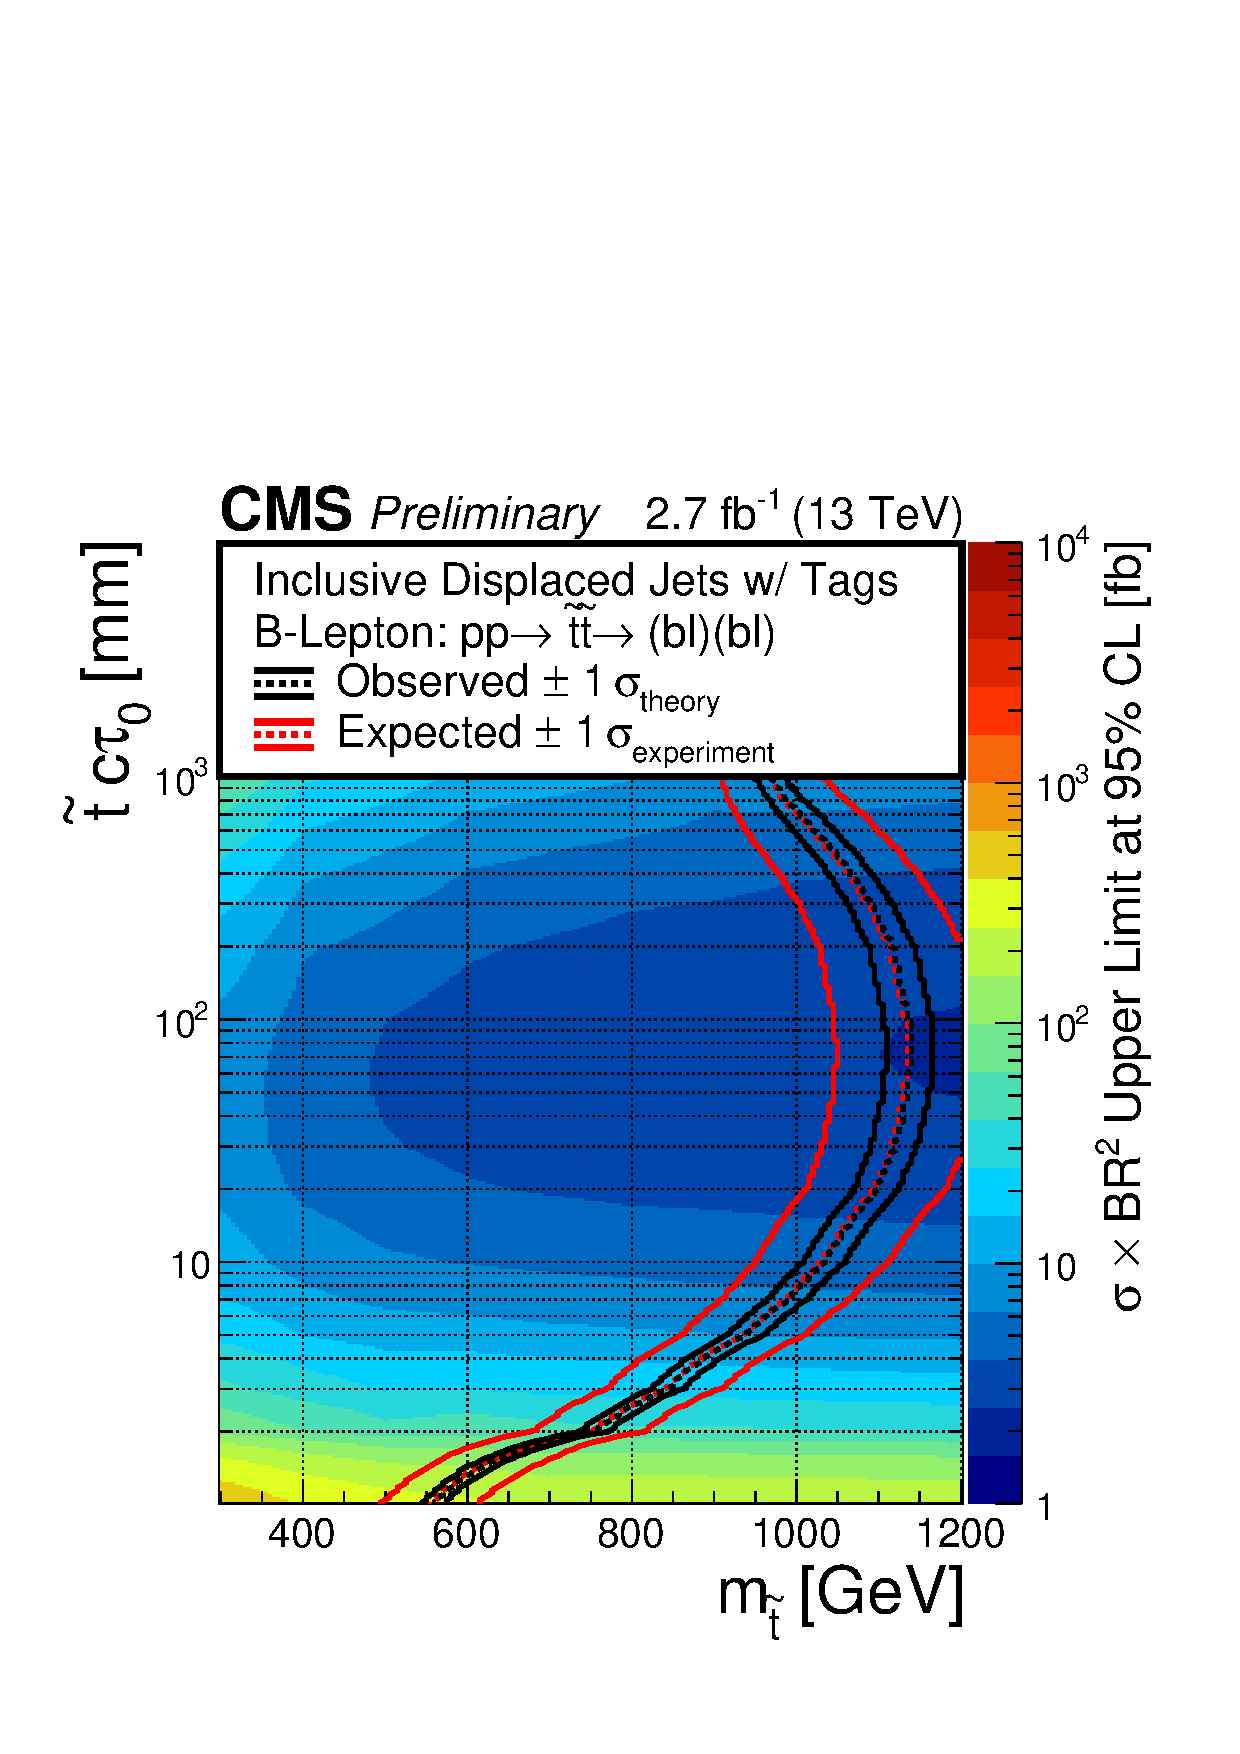
\includegraphics[width=.75\textwidth]{figures/pas//RESULT/UNBLINDED_LIMITS/B-Lepton2D.pdf}
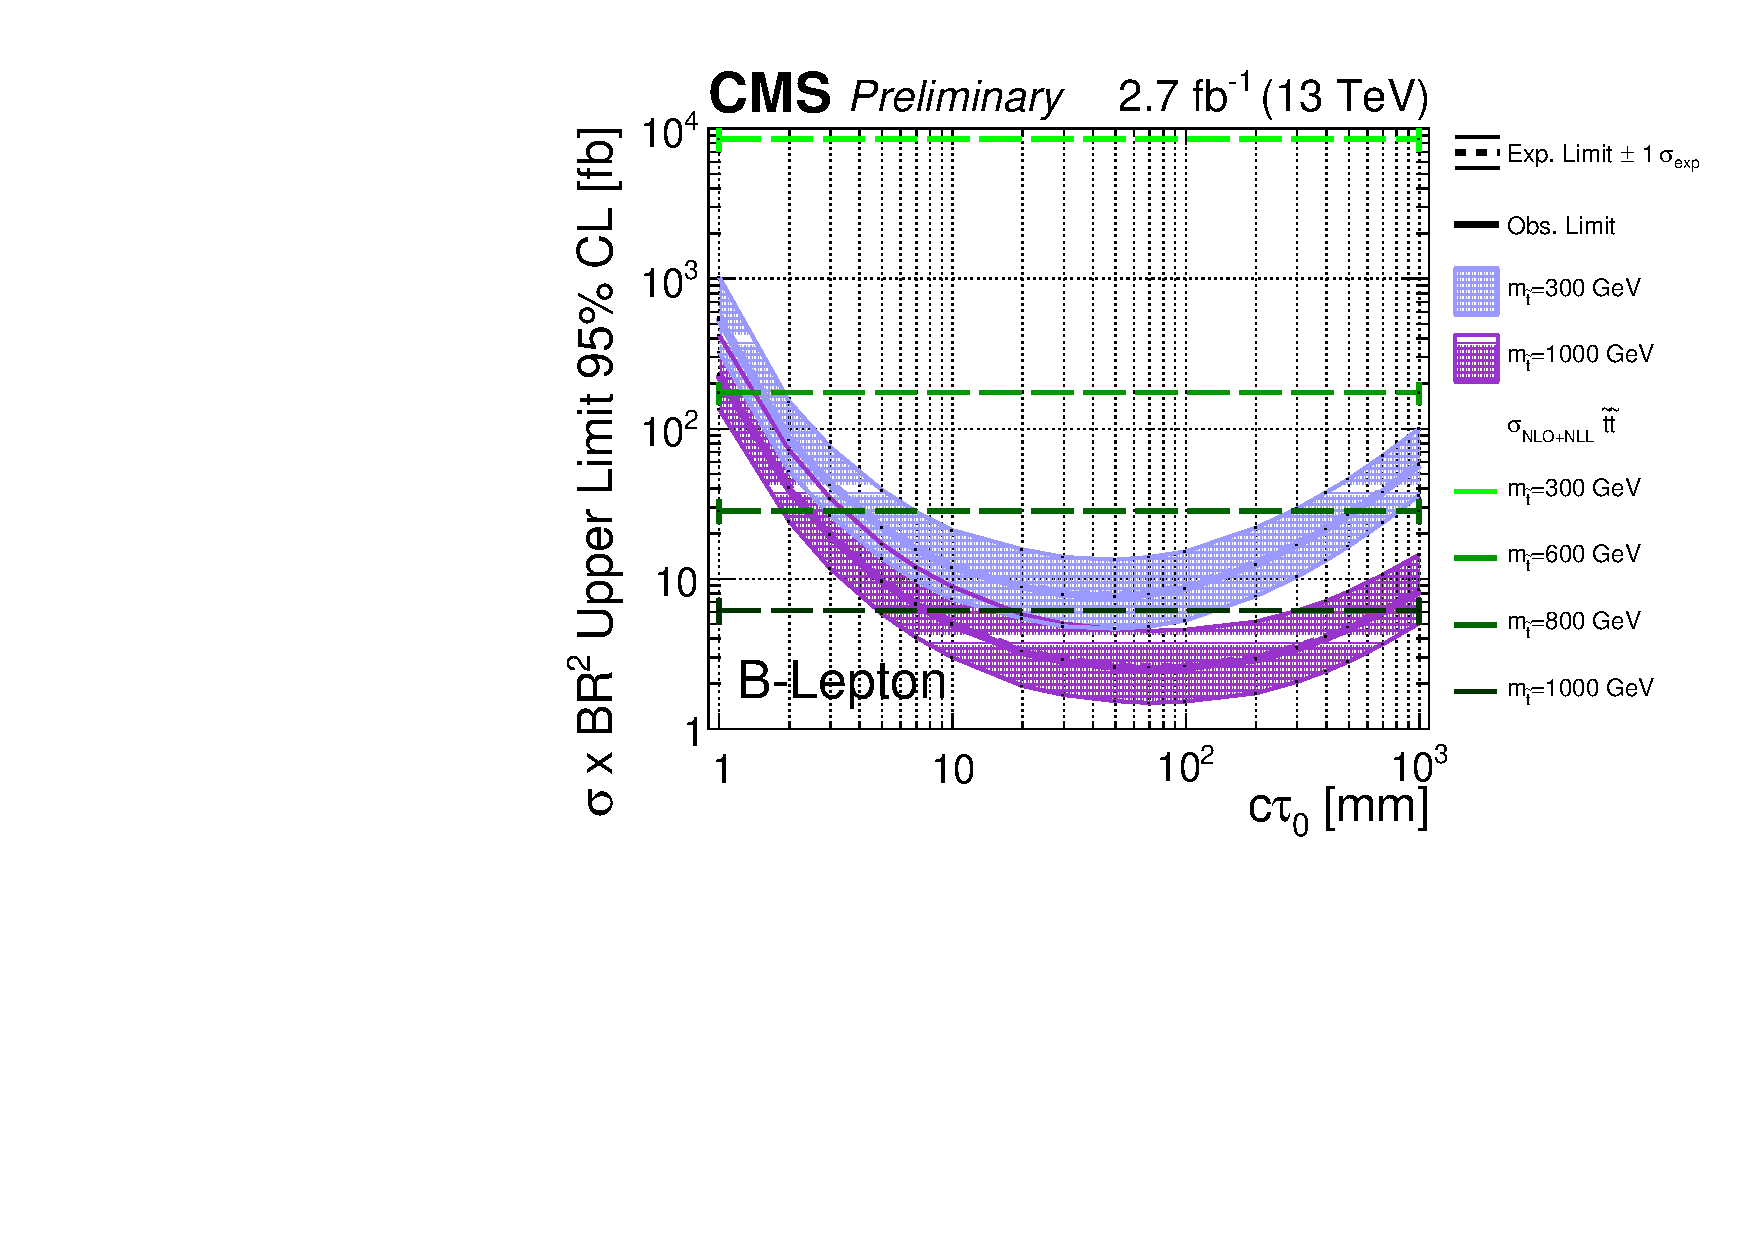
\includegraphics[width=.75\textwidth]{figures/pas//RESULT/UNBLINDED_LIMITS/B-Lepton.pdf}
\caption{The excluded cross section at 95\% CL for the B-Lepton model
  as a function of the mass and lifetime of the parent particle
  $\tilde{t}$ (top) and as a function of the lifetime for two values
  of the mass (bottom).  The bottom plot also shows the expected upper
  limits with one standard deviation
  uncertainties.\label{fig:dsusy_limit_lepton}}
\end{center}
\end{figure}

\begin{figure}[tb]
\begin{center}
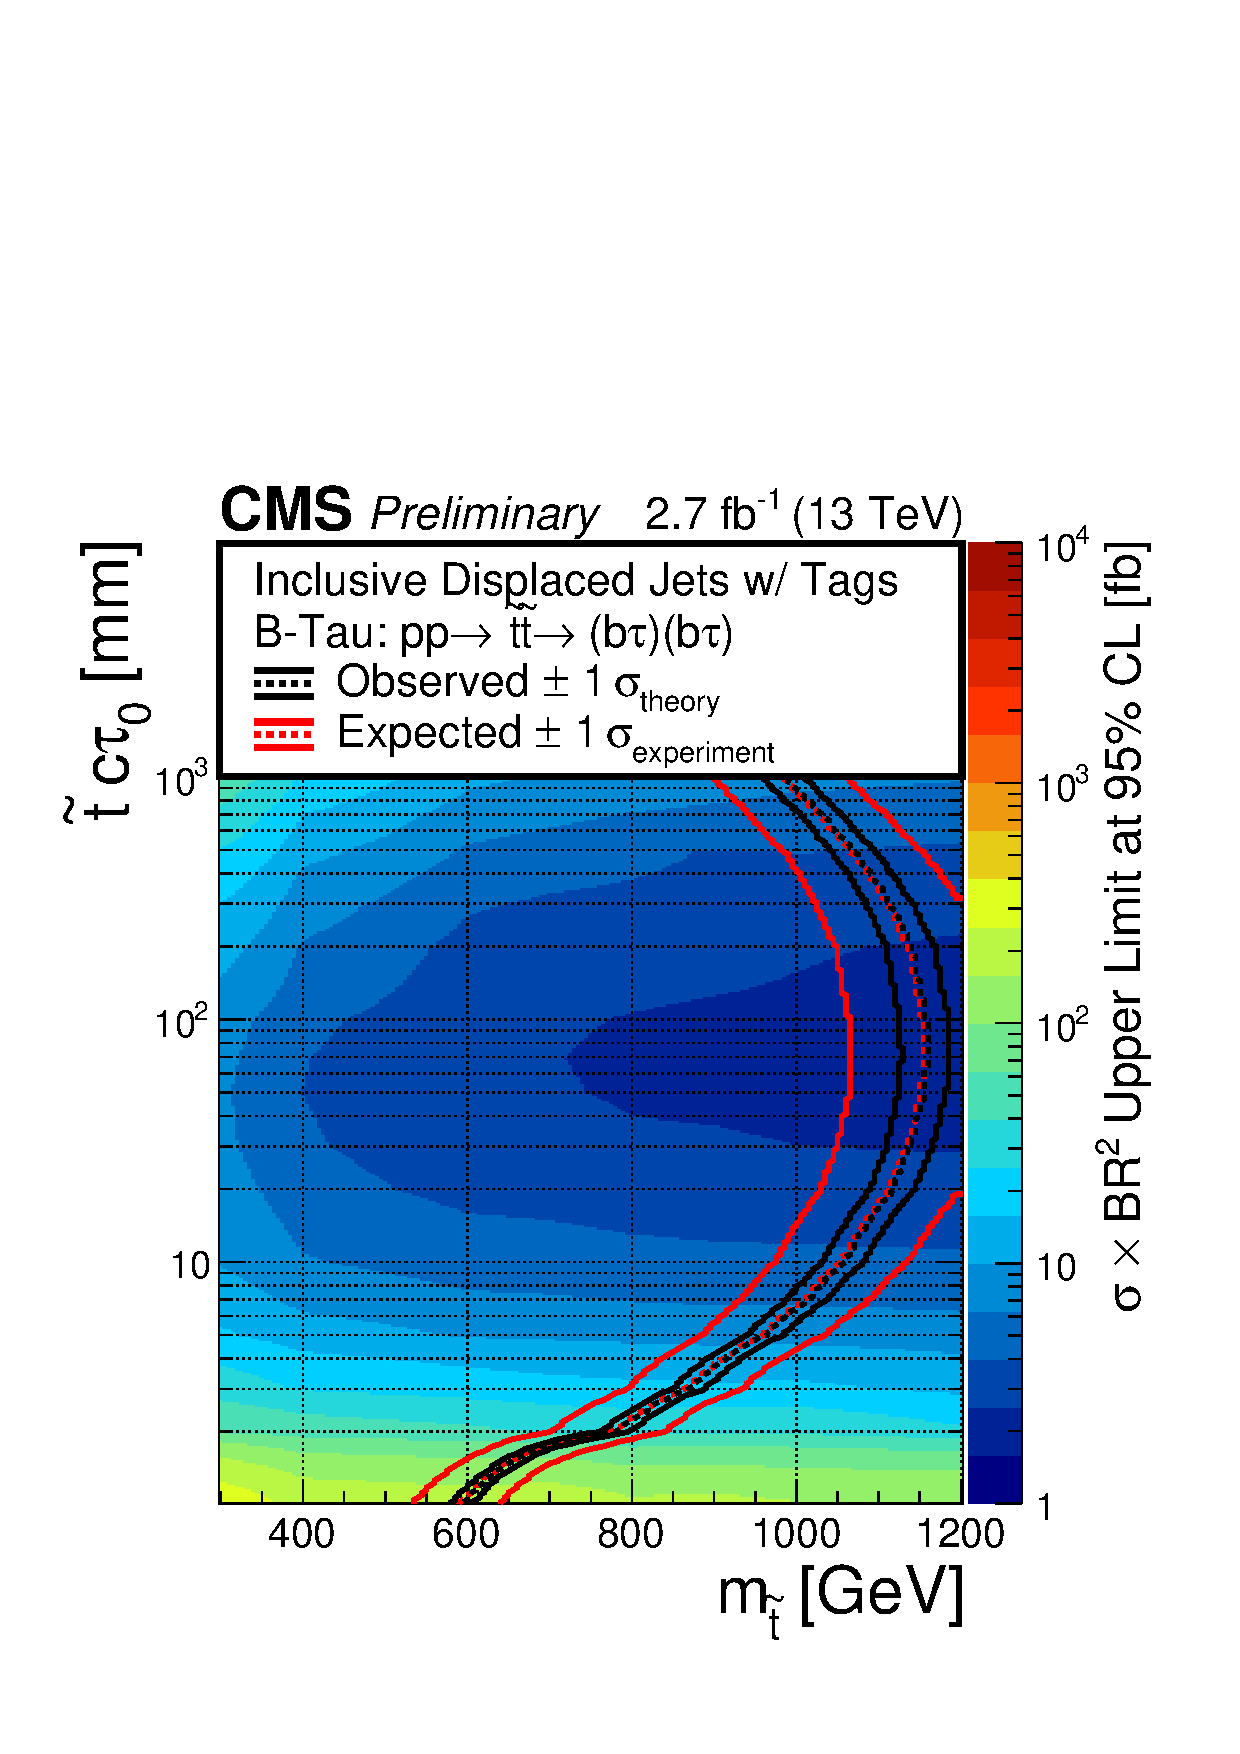
\includegraphics[width=.75\textwidth]{figures/pas//RESULT/UNBLINDED_LIMITS/B-Tau2D.pdf}
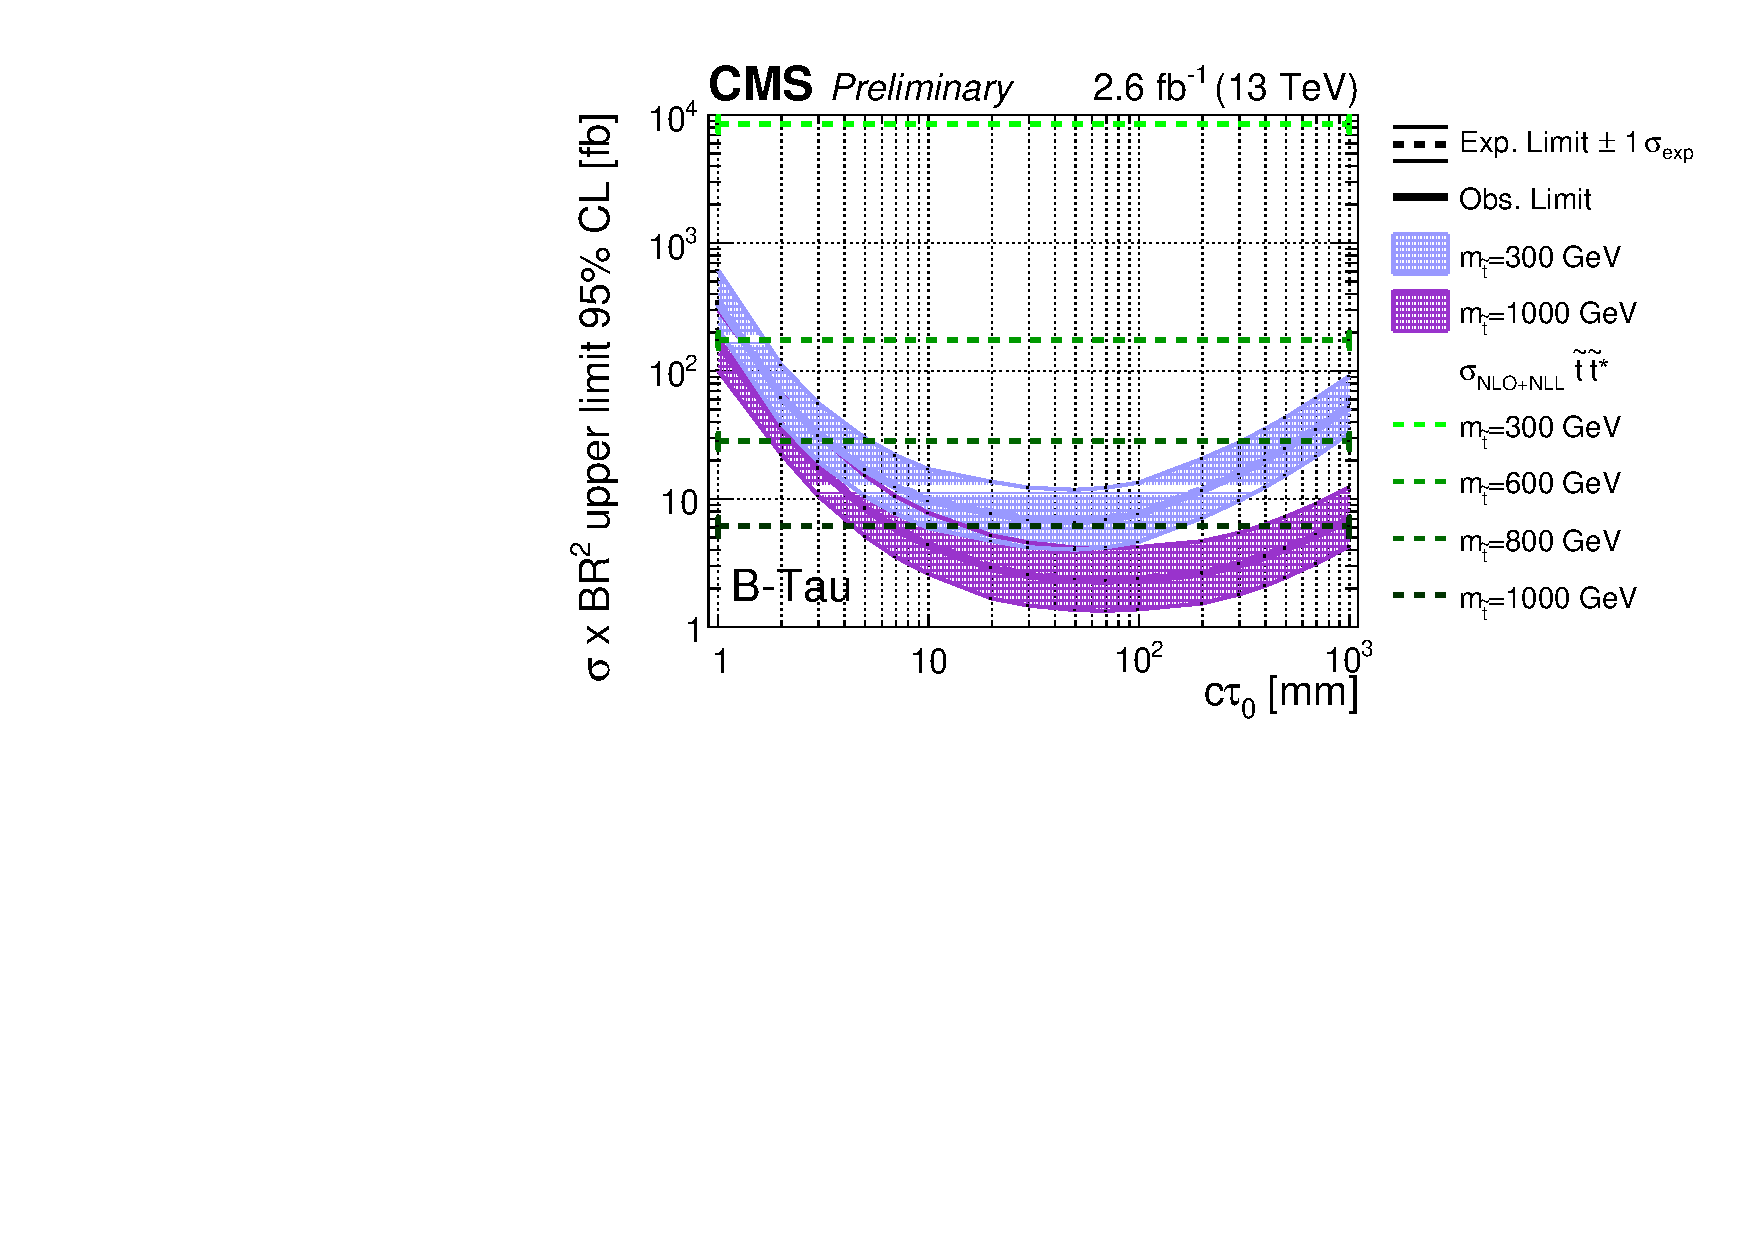
\includegraphics[width=.75\textwidth]{figures/pas//RESULT/UNBLINDED_LIMITS/B-Tau.pdf}
\caption{The excluded cross section at 95\% CL for the B-Tau model as
  a function of the mass and lifetime of the parent particle
  $\tilde{t}$ (top) and as a function of the lifetime for two values
  of the mass (bottom).  The bottom plot also shows the expected upper
  limits with one standard deviation
  uncertainties.\label{fig:dsusy_limit_tau}}
\end{center}
\end{figure}

\begin{figure}[tb]
\begin{center}
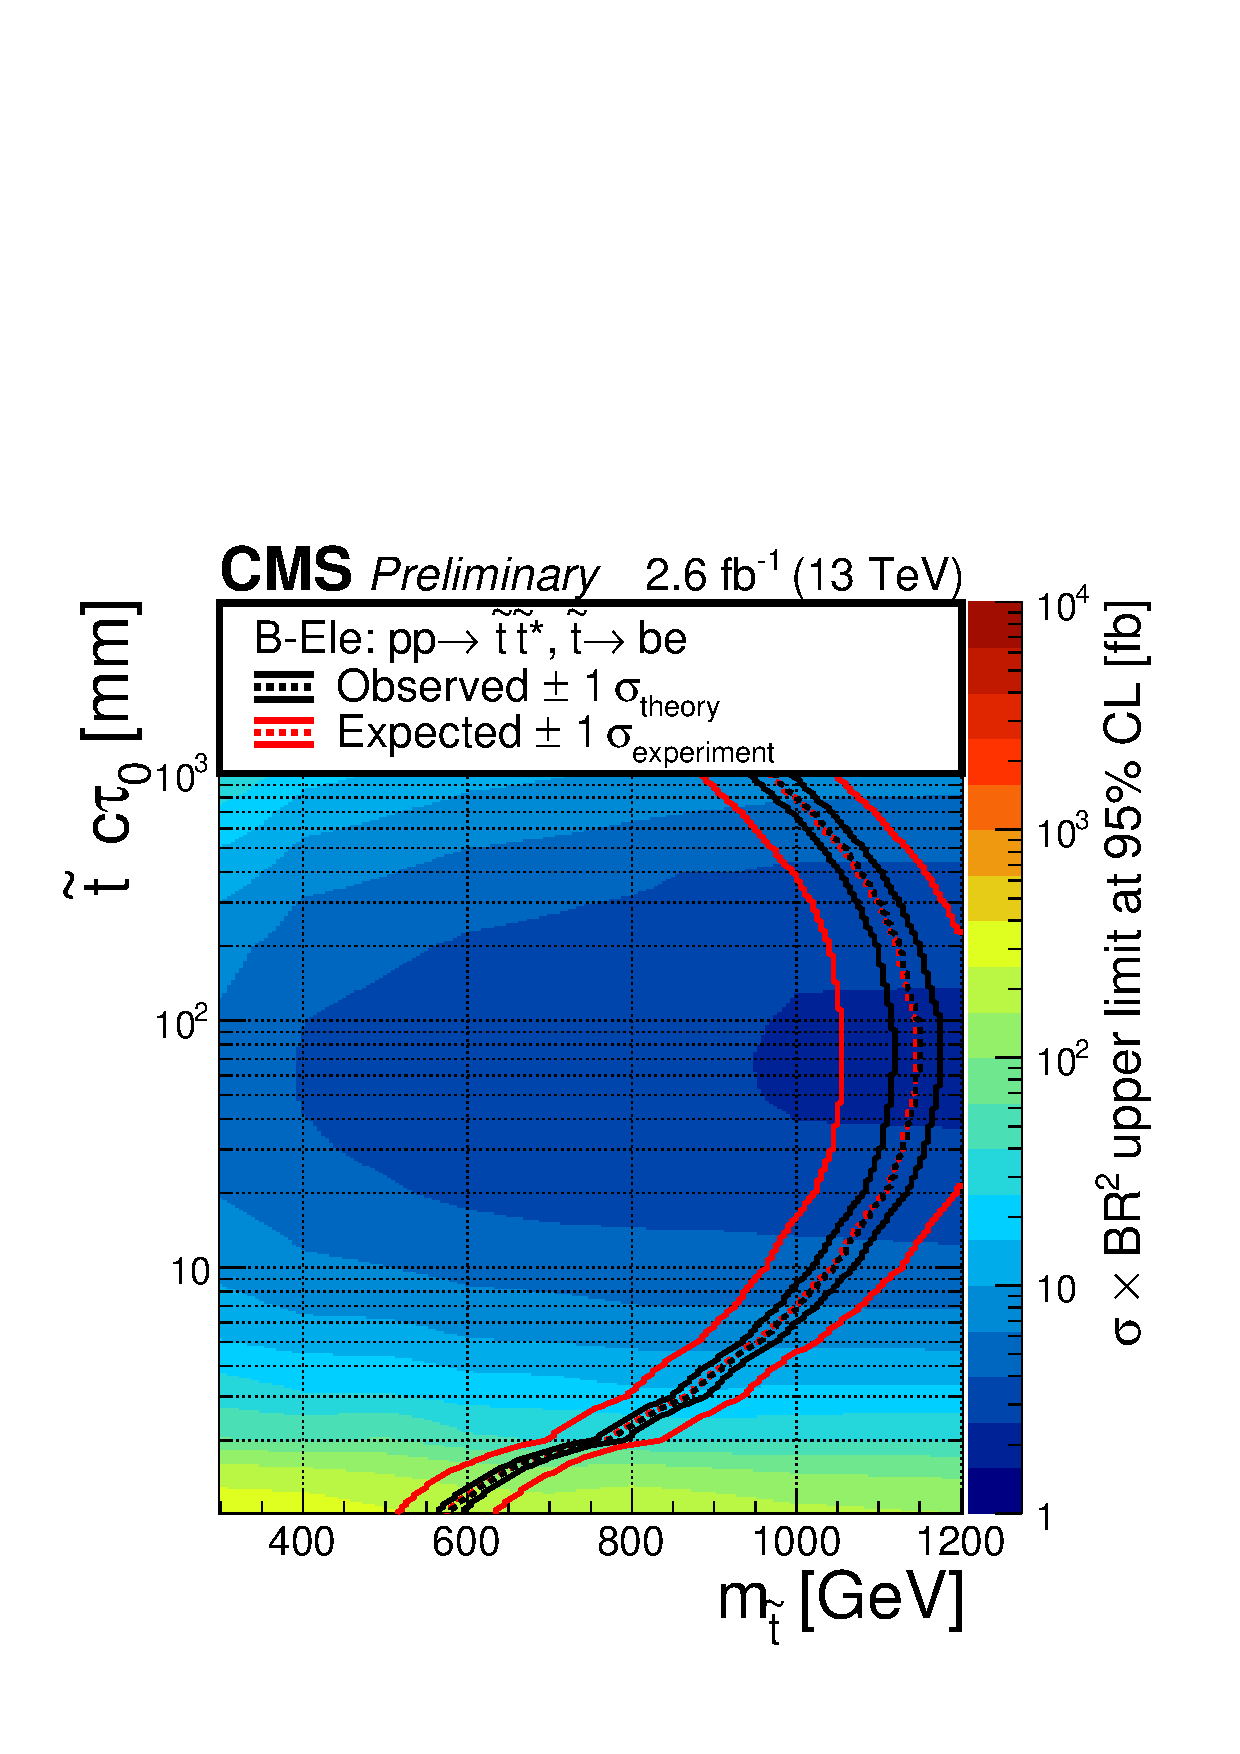
\includegraphics[width=.75\textwidth]{figures/pas//RESULT/UNBLINDED_LIMITS/B-Ele2D.pdf}
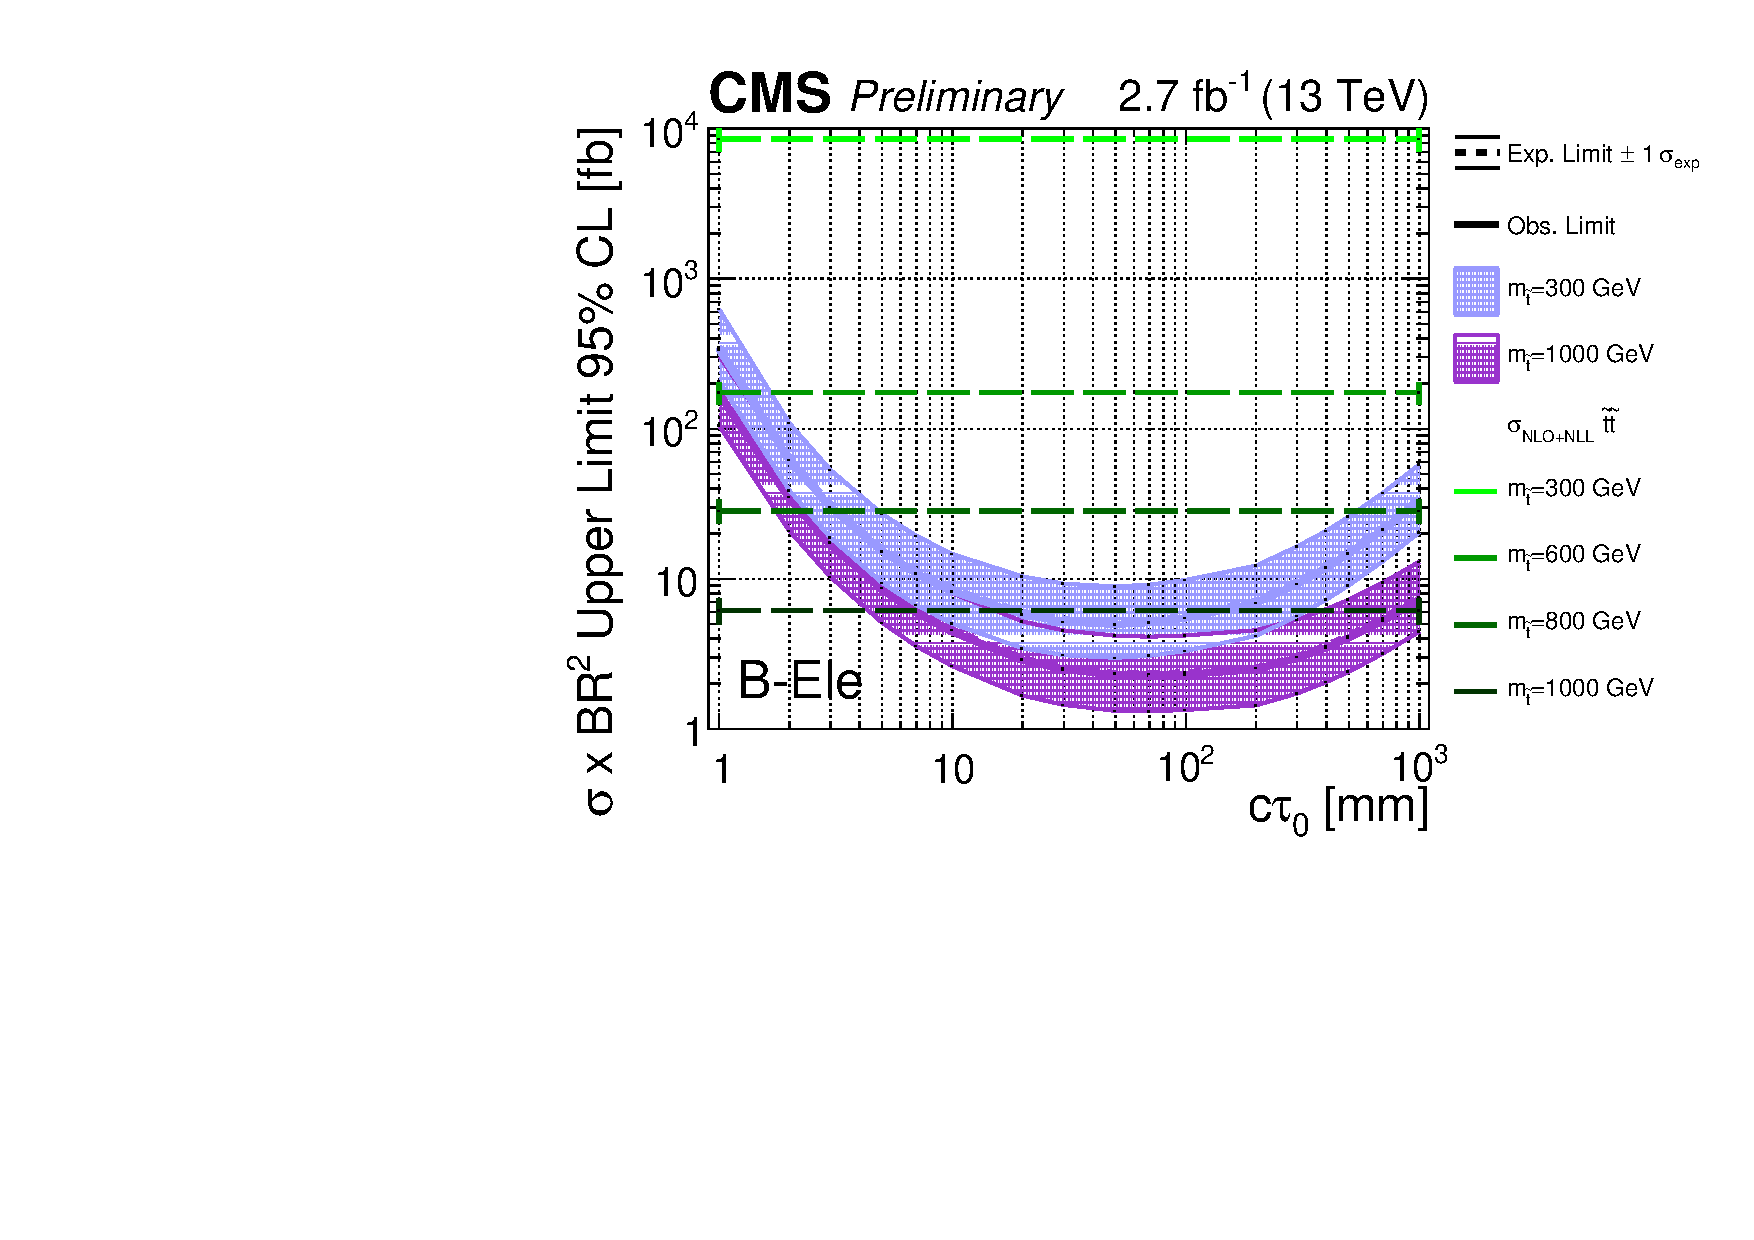
\includegraphics[width=.75\textwidth]{figures/pas//RESULT/UNBLINDED_LIMITS/B-Ele.pdf}
\caption{ The excluded cross section at 95\% CL for the B-Ele model as
  a function of the mass and lifetime of the parent particle
  $\tilde{t}$ (top) and as a function of the lifetime for four values
  of the mass (bottom).  The bottom plot also shows the expected upper
  limits with one standard deviation
  uncertainties.\label{fig:dsusy_limit_ele}}
\end{center}
\end{figure}

\begin{figure}[tb]
\begin{center}
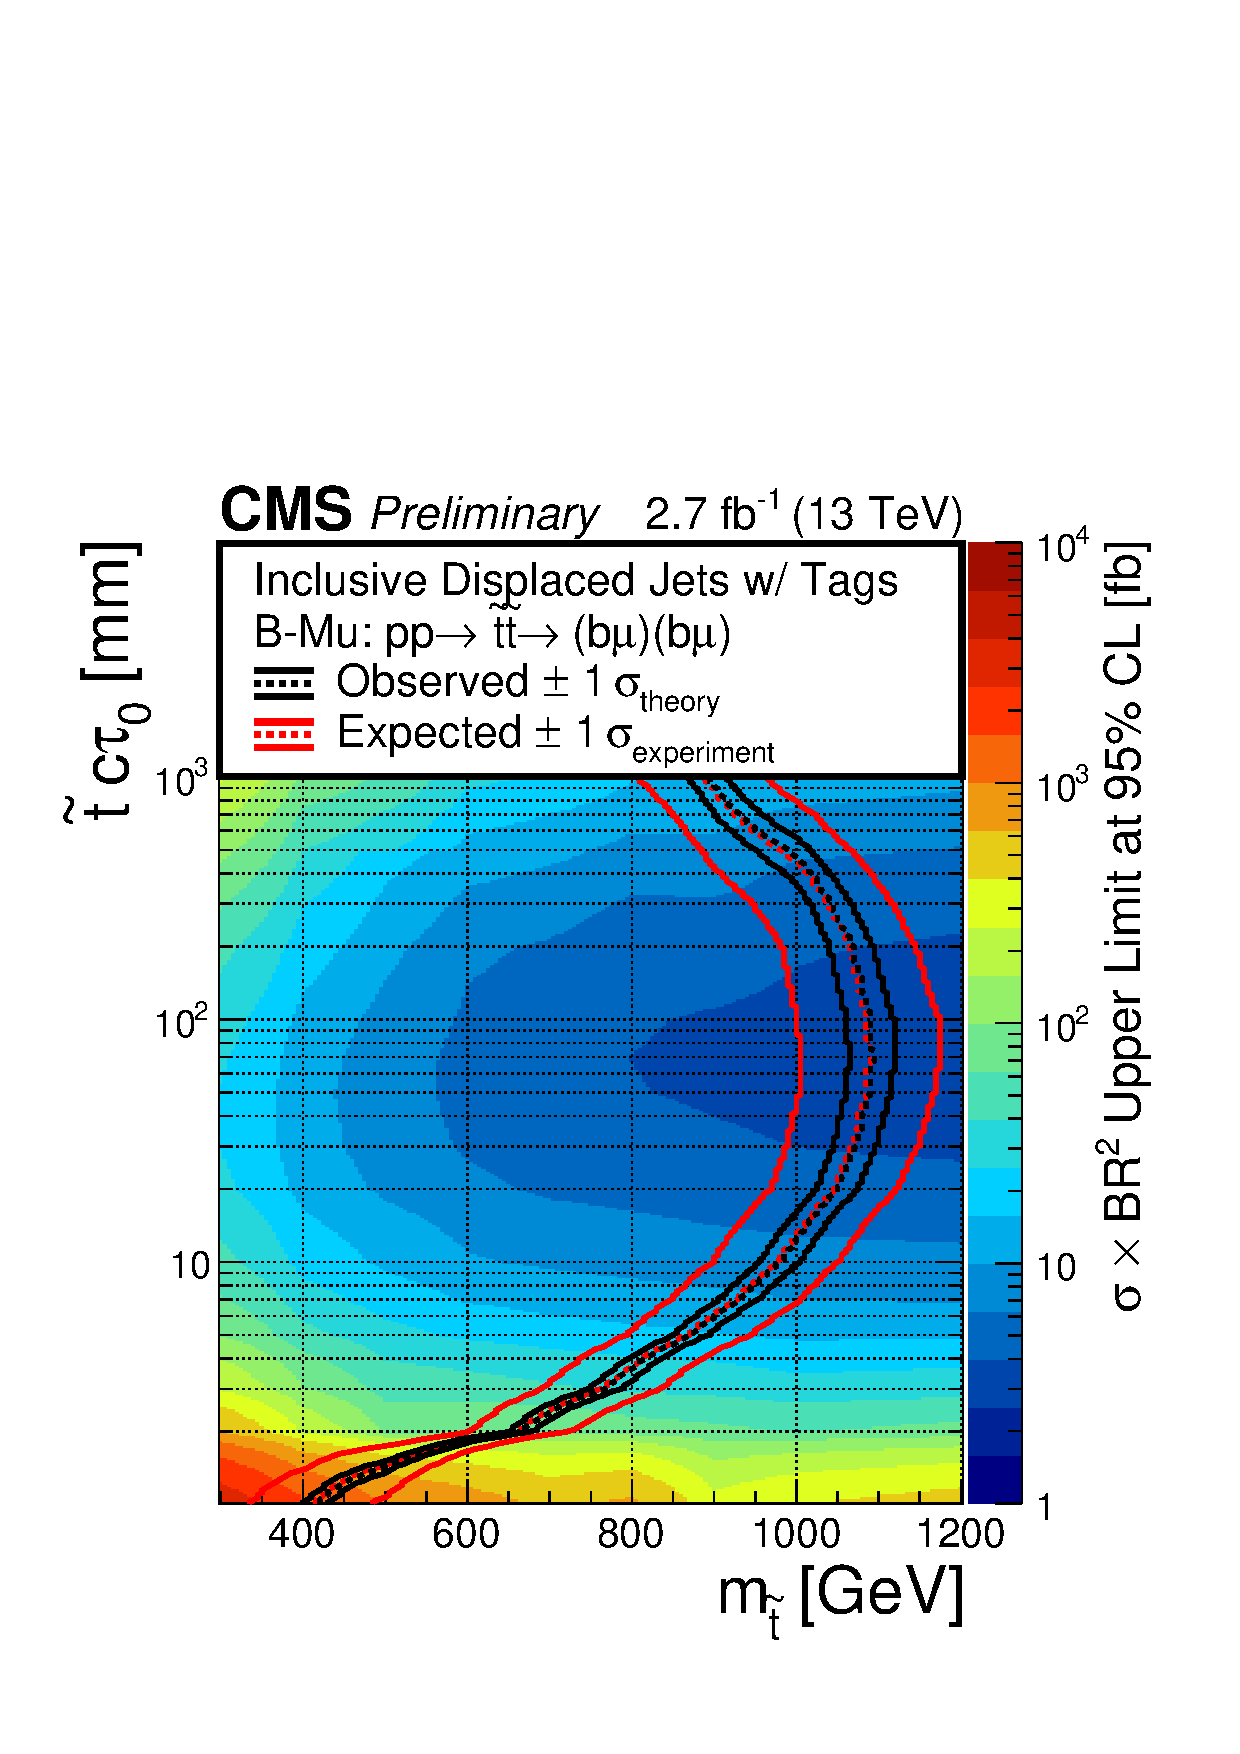
\includegraphics[width=.75\textwidth]{figures/pas//RESULT/UNBLINDED_LIMITS/B-Mu2D.pdf}
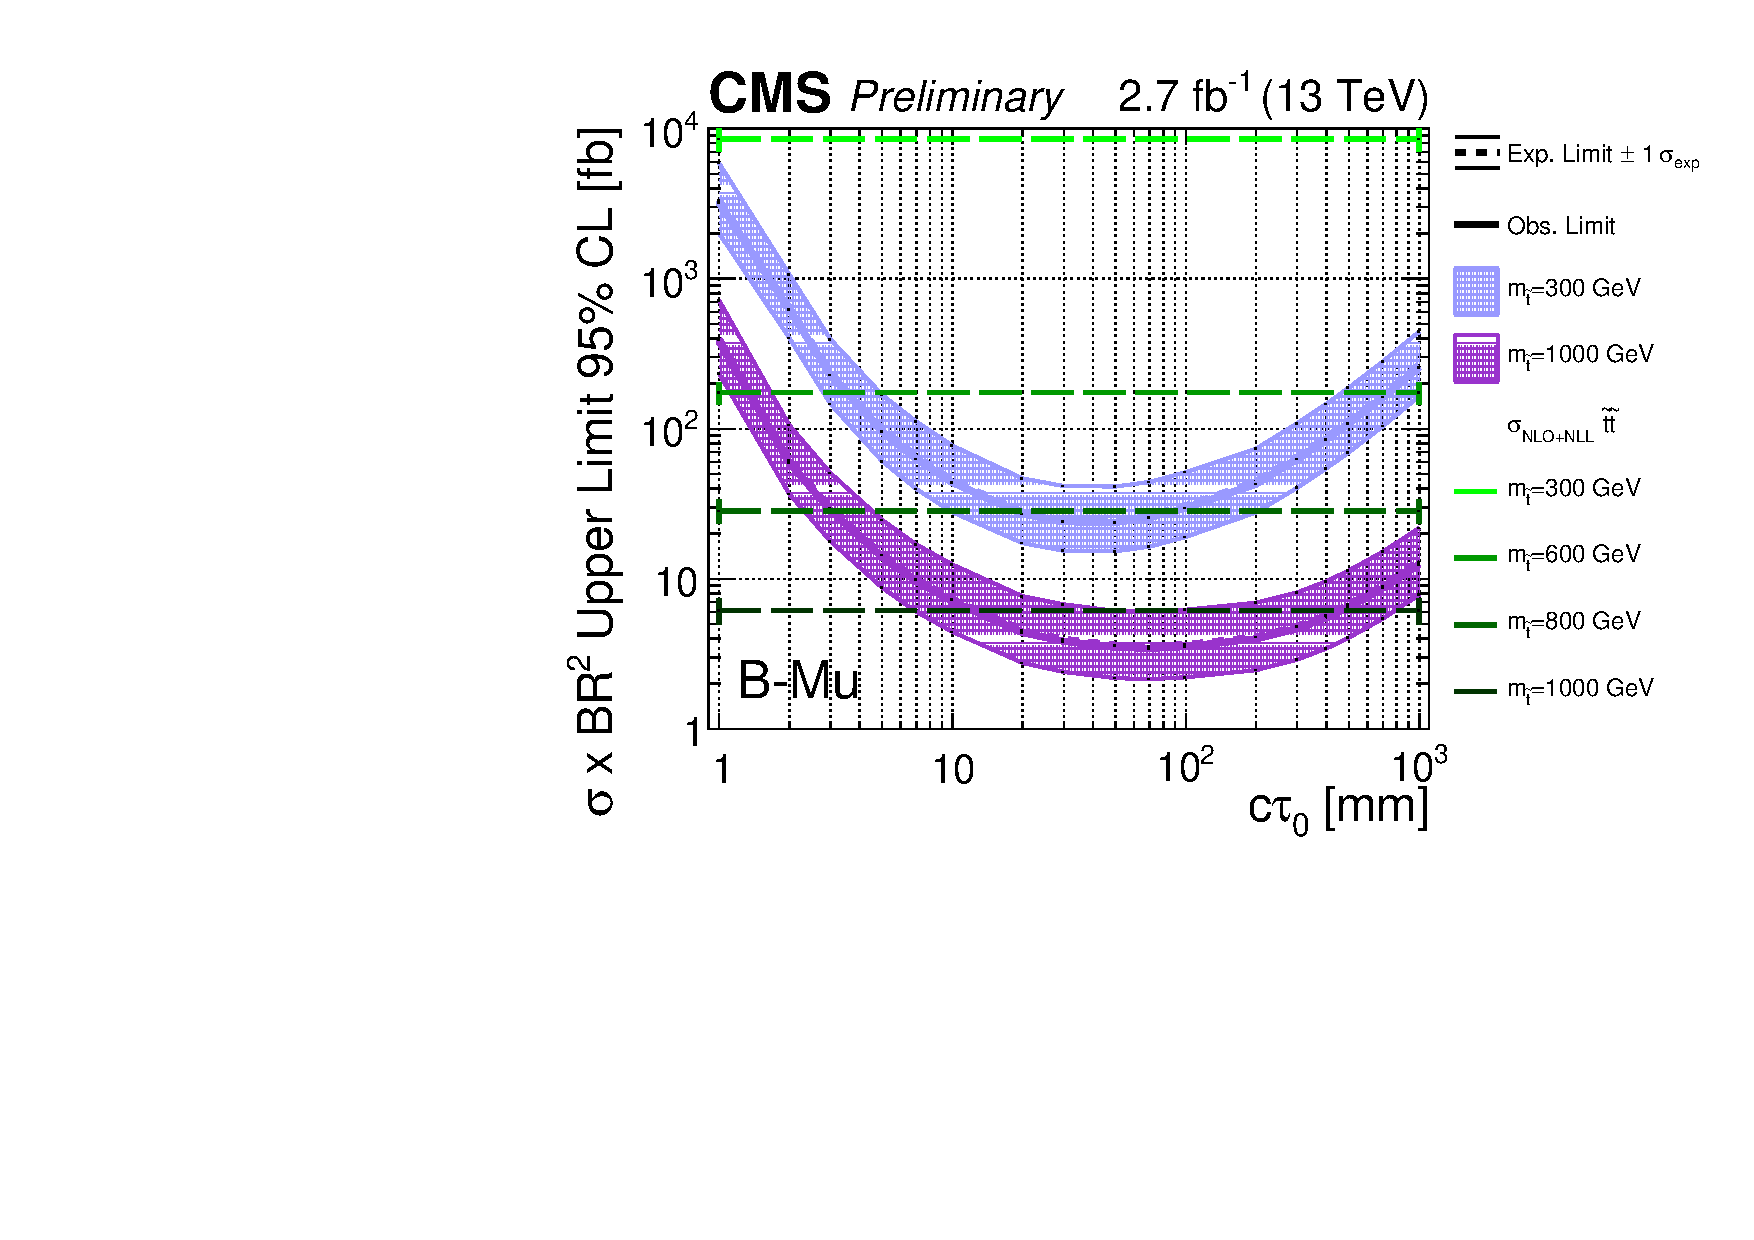
\includegraphics[width=.75\textwidth]{figures/pas//RESULT/UNBLINDED_LIMITS/B-Mu.pdf}
\caption{ The excluded cross section at 95\% CL for the B-Mu model as
  a function of the mass and lifetime of the parent particle
  $\tilde{t}$ (top) and as a function of the lifetime for four values
  of the mass (bottom).  The bottom plot also shows the expected upper
  limits with one standard deviation
  uncertainties.\label{fig:dsusy_limit_mu}}
\end{center}
\end{figure}
